\documentclass[11pt]{report}
% Shared preamble for CSAI321 Computer Networks notes
\usepackage[a4paper,margin=2.2cm]{geometry}
\usepackage[T1]{fontenc}
\usepackage{lmodern}
\usepackage{amsmath,amssymb,pifont}
\usepackage{xcolor}
\usepackage{tikz}
\usetikzlibrary{arrows.meta,shapes.symbols,shapes.geometric,positioning,shapes.geometric,shapes.misc,calc,fit,backgrounds,decorations.pathreplacing,matrix}
\usepackage[most]{tcolorbox}
\usepackage{booktabs,tabularx,array,longtable}
\usepackage{enumitem}
\usepackage{listings}
\usepackage{hyperref}
\usepackage{titlesec}
\hypersetup{colorlinks=true,linkcolor=blue!50!black,urlcolor=blue!60!black}
\setlist{itemsep=2pt,topsep=4pt}
\setlength{\parindent}{0pt}
\setlength{\parskip}{5pt}
\renewcommand{\arraystretch}{1.3}

\definecolor{cnblue}{HTML}{1F4E9A}
\definecolor{cngreen}{HTML}{2E7D32}
\definecolor{cnorange}{HTML}{E65100}
\definecolor{cnpurple}{HTML}{6A1B9A}
\definecolor{cnred}{HTML}{C62828}
\definecolor{cngrey}{HTML}{F4F6FA}

\titleformat{\section}{\Large\bfseries\color{cnblue}}{\thesection}{0.8em}{}
\titleformat{\subsection}{\large\bfseries\color{cnblue!80!black}}{\thesubsection}{0.8em}{}

\newtcolorbox{keyidea}[1][Key idea]{enhanced,breakable,colback=cnblue!5,colframe=cnblue,fonttitle=\bfseries,title={#1}}
\newtcolorbox{analogy}[1][Analogy]{enhanced,breakable,colback=cngreen!5,colframe=cngreen,fonttitle=\bfseries,title={#1}}
\newtcolorbox{examtip}[1][Exam tip]{enhanced,breakable,colback=cnorange!6,colframe=cnorange,fonttitle=\bfseries,title={#1}}
\newtcolorbox{workedex}[1][Worked example]{enhanced,breakable,colback=cnpurple!4,colframe=cnpurple,fonttitle=\bfseries,title={#1}}
\newtcolorbox{recap}[1][Quick revision]{enhanced,breakable,colback=cngrey,colframe=black!60,fonttitle=\bfseries,title={#1}}

\lstset{basicstyle=\ttfamily\small,backgroundcolor=\color{cngrey},frame=single,rulecolor=\color{black!25},columns=fullflexible,breaklines=true,keepspaces=true}

% TikZ styles
\tikzset{
  box/.style={draw,rounded corners=3pt,minimum height=8mm,minimum width=22mm,align=center,font=\small},
  host/.style={draw,fill=cnblue!10,rounded corners=2pt,minimum width=14mm,minimum height=9mm,align=center,font=\small},
  srv/.style={draw,fill=cngreen!12,rounded corners=2pt,minimum width=14mm,minimum height=11mm,align=center,font=\small},
  rtr/.style={draw,circle,fill=cnorange!15,minimum size=9mm,font=\small,inner sep=1pt},
  arr/.style={-{Stealth[length=2.5mm]},thick},
  darr/.style={{Stealth[length=2.5mm]}-{Stealth[length=2.5mm]},thick},
  msg/.style={-{Stealth[length=2mm]},thick,every node/.append style={fill=white,inner sep=1.2pt,sloped}},
  lbl/.style={font=\footnotesize,fill=white,inner sep=1pt},
}
% sequence-diagram helper: \lifelines{x1}{x2}{top}{bottom}
\newcommand{\lifelines}[4]{\draw[dashed,gray] (#1,#3) -- (#1,#4); \draw[dashed,gray] (#2,#3) -- (#2,#4);}
\titleformat{\chapter}[display]{\bfseries\color{cnblue}}{\large CSAI321 Computer Networks \textbullet{} Notes}{4pt}{\Huge}[\vspace{2pt}{\color{cnblue}\titlerule[1.2pt]}]
\titlespacing*{\chapter}{0pt}{-25pt}{18pt}

\begin{document}
\begin{titlepage}
\centering
\vspace*{3cm}
{\Huge\bfseries\color{cnblue} CSAI321 Computer Networks\par}
\vspace{0.6cm}
{\LARGE Lecture Notes: Lectures 1--10\par}
\vspace{0.8cm}
{\large End-semester revision, explained simply with diagrams\par}
\vspace{2cm}
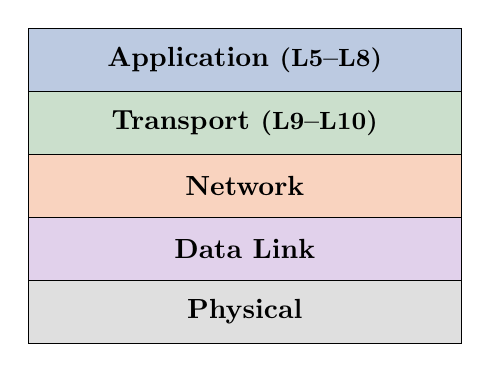
\begin{tikzpicture}[L/.style={draw,minimum width=55mm,minimum height=8mm,font=\bfseries}]
  \node[L,fill=cnblue!30] at (0,0) {Application \small(L5--L8)};
  \node[L,fill=cngreen!25] at (0,-0.8) {Transport \small(L9--L10)};
  \node[L,fill=cnorange!25] at (0,-1.6) {Network};
  \node[L,fill=cnpurple!20] at (0,-2.4) {Data Link};
  \node[L,fill=gray!25] at (0,-3.2) {Physical};
\end{tikzpicture}
\vfill
{\small Box legend: \textcolor{cnblue}{\textbf{Key idea}} \quad \textcolor{cngreen}{\textbf{Analogy}} \quad \textcolor{cnorange}{\textbf{Exam tip}} \quad \textcolor{cnpurple}{\textbf{Worked example}} \quad \textbf{Quick revision}\par}
\end{titlepage}
\tableofcontents
\chapter{Lecture 1 --- Introduction to Computer Networks}

\begin{keyidea}[The one idea from this lecture]
``The cloud'' is not magic and not weightless. It is millions of real computers in real buildings, joined by real cables (many under the sea). A \textbf{computer network} is what lets all of these machines talk to each other. This course explains, step by step, how that talking happens.
\end{keyidea}

\section{What is the cloud?}

A common joke says ``the cloud is just someone else's computer''. The lecture's answer: it is more like \emph{a lot} of someone else's computers.

\begin{itemize}
  \item Cloud providers such as \textbf{AWS} (Amazon Web Services), \textbf{Azure} (Microsoft) and \textbf{GCP} (Google Cloud Platform) run huge \textbf{data centres}. The lecture showed Google's data centre in Council Bluffs, Iowa: rows and rows of servers.
  \item All those servers must constantly \textbf{talk to each other} and to you. So every cloud provider owns a super-fast computer network.
  \item The job of that network: get all those 0s and 1s to you \textbf{efficiently}.
\end{itemize}

\begin{center}
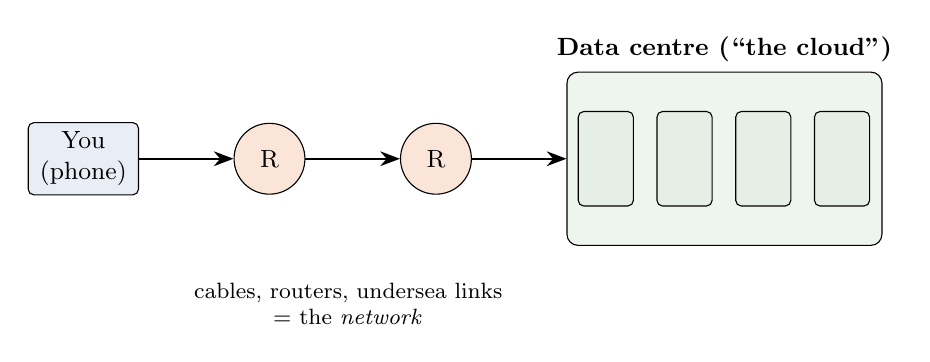
\begin{tikzpicture}[node distance=6mm]
  \node[host] (u) {You\\(phone)};
  \node[rtr, right=12mm of u] (r1) {R};
  \node[rtr, right=12mm of r1] (r2) {R};
  \node[draw,rounded corners,fill=cngreen!8,right=12mm of r2,minimum width=40mm,minimum height=22mm] (dc) {};
  \node[above=0mm of dc.north,font=\small\bfseries] {Data centre (``the cloud'')};
  \foreach \i in {0,1,2,3} { \node[srv,minimum width=7mm,minimum height=12mm] at ($(dc.west)+(5mm+\i*10mm,0)$) {}; }
  \draw[arr] (u) -- (r1); \draw[arr] (r1) -- (r2); \draw[arr] (r2) -- (dc);
  \node[below=10mm of r1,font=\footnotesize,align=center,xshift=10mm] {cables, routers, undersea links\\= the \emph{network}};
\end{tikzpicture}
\end{center}

\section{Networks are not new}

\begin{itemize}
  \item In the \textbf{1960s} (1969, ARPANET), a computer at \textbf{UCLA} tried to send the word \texttt{login} to a computer at the \textbf{Stanford Research Institute}.
  \item Only \texttt{lo} got through before the system crashed. So the very first message on the ancestor of the internet was ``lo''!
  \item Lesson: networking has always been hard, and things go wrong. Much of this course is about how networks cope with failures.
\end{itemize}

\section{Types of network by size}

Traditionally, networks are classified by how much area they cover.

\begin{center}
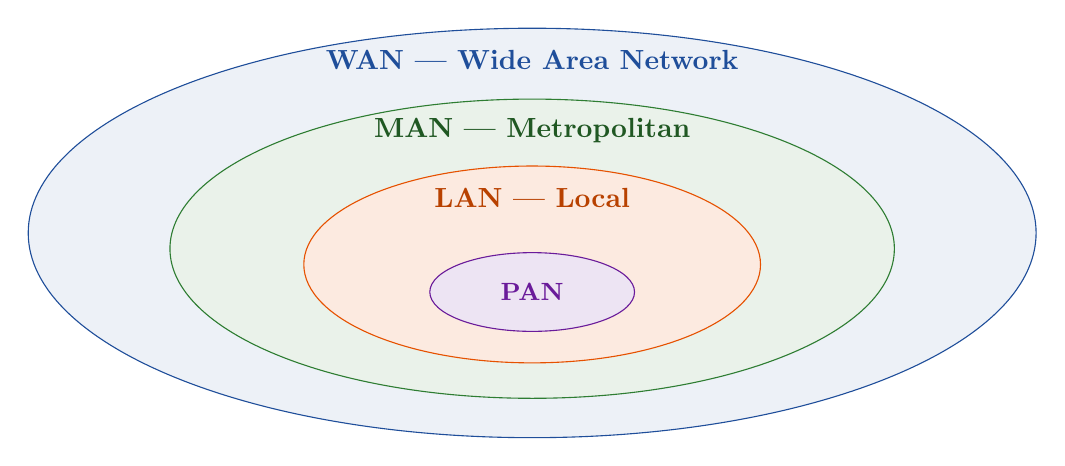
\begin{tikzpicture}
  \draw[fill=cnblue!8,draw=cnblue] (0,0) ellipse (6.4cm and 2.6cm);
  \node[font=\bfseries,cnblue] at (0,2.2) {WAN --- Wide Area Network};
  \draw[fill=cngreen!10,draw=cngreen] (0,-0.2) ellipse (4.6cm and 1.9cm);
  \node[font=\bfseries,cngreen!70!black] at (0,1.3) {MAN --- Metropolitan};
  \draw[fill=cnorange!12,draw=cnorange] (0,-0.4) ellipse (2.9cm and 1.25cm);
  \node[font=\bfseries,cnorange!80!black] at (0,0.45) {LAN --- Local};
  \draw[fill=cnpurple!12,draw=cnpurple] (0,-0.75) ellipse (1.3cm and 0.5cm);
  \node[font=\bfseries\small,cnpurple] at (0,-0.75) {PAN};
\end{tikzpicture}
\end{center}

\begin{center}
\begin{tabularx}{\textwidth}{>{\bfseries}l l X}
\toprule
Type & Range & Example \\
\midrule
PAN (Personal Area Network) & A few metres & Phone $\leftrightarrow$ smartwatch, Bluetooth headphones \\
LAN (Local Area Network) & A room / building & Your home WiFi, an office or college lab \\
MAN (Metropolitan Area Network) & A city & City-wide networks run by a municipality or big organisation \\
WAN (Wide Area Network) & Countries / continents & Branch offices of a company joined together; the \textbf{internet} itself \\
\bottomrule
\end{tabularx}
\end{center}

\begin{examtip}
Remember the order from smallest to largest: \textbf{P}AN $<$ \textbf{L}AN $<$ \textbf{M}AN $<$ \textbf{W}AN. The internet is the biggest WAN of all.
\end{examtip}

\section{The internet is physical}

Even though we call it ``the cloud'', the internet sits on a massive \textbf{physical infrastructure}.

\begin{itemize}
  \item In 2025 there were about \textbf{597 submarine (undersea) cable systems} linking continents.
  \item Most international traffic travels through these fibre-optic cables lying on the ocean floor, not through satellites.
\end{itemize}

\subsection{Why is it hard to keep the cables safe?}
\begin{itemize}
  \item \textbf{Fishing anchors and trawlers:} the most common cause of damage to trans-Atlantic cables is ships' anchors accidentally dragging across and cutting them.
  \item \textbf{Sharks} have been filmed biting cables (the lecture's fun example).
  \item The cables are thousands of kilometres long and sit in deep water, so they are hard to watch and slow to repair.
\end{itemize}

\section{``What happens when\ldots?'' --- the gap this course fills}

\subsection{Tapping the Instagram icon}
You tap Instagram and a reel plays in under a second. Most people would describe this as ``WiFi $\to$ Instagram''. In reality the data passes through your phone's software, the WiFi radio, your home router, your ISP, many routers across the internet, possibly an undersea cable, a load balancer, a server in a data centre, a cache/CDN and back.

\begin{center}
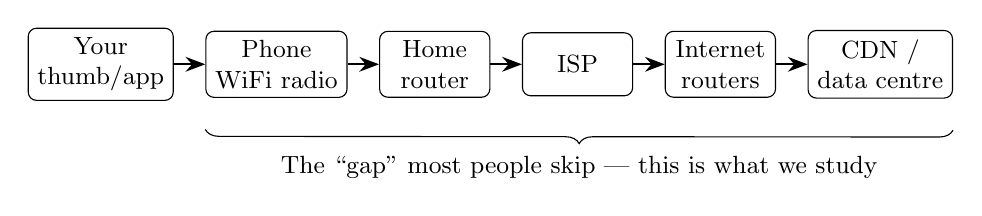
\begin{tikzpicture}[node distance=4mm,every node/.style={font=\scriptsize}]
  \node[box,minimum width=14mm] (a) {Your\\thumb/app};
  \node[box,minimum width=14mm,right=of a] (b) {Phone\\WiFi radio};
  \node[box,minimum width=14mm,right=of b] (c) {Home\\router};
  \node[box,minimum width=14mm,right=of c] (d) {ISP};
  \node[box,minimum width=14mm,right=of d] (e) {Internet\\routers};
  \node[box,minimum width=14mm,right=of e] (f) {CDN /\\data centre};
  \foreach \x/\y in {a/b,b/c,c/d,d/e,e/f} \draw[arr] (\x) -- (\y);
  \draw[decorate,decoration={brace,mirror,amplitude=5pt}] ([yshift=-4mm]b.south west) -- ([yshift=-4mm]f.south east) node[midway,below=6pt,font=\small] {The ``gap'' most people skip --- this is what we study};
\end{tikzpicture}
\end{center}

\subsection{The 10 PM Netflix problem}
At 10 PM millions of people start a Netflix movie at the same time. Suddenly the app buffers or fails. Why? Too many people share the same links and servers at once (congestion), packets queue up and get delayed or dropped. Understanding \emph{why} this happens and how networks fight it is a central goal of the course.

\section{Objective of the course}
\begin{itemize}
  \item To \textbf{demystify} how networks work, because networks are everywhere.
  \item Even modern AI depends on networks: thousands of \textbf{GPUs} in a training cluster are connected with very fast network cards. A slow network means slow training.
  \item What to expect: \textbf{foundations} (how computing devices talk to each other, how data travels), \textbf{hands-on labs} (configure your own network) and \textbf{network security}.
\end{itemize}

\section{The top-down approach}

The course follows the \textbf{top-down approach} (as in the Kurose \& Ross textbook): start at the layer you already use, then dig down.

\begin{center}
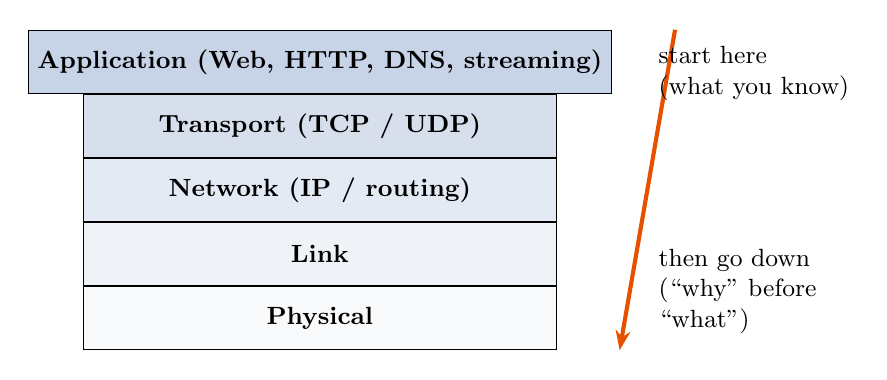
\begin{tikzpicture}[layer/.style={draw,minimum width=60mm,minimum height=8mm,font=\small\bfseries}]
  \node[layer,fill=cnblue!25] (a) {Application (Web, HTTP, DNS, streaming)};
  \node[layer,fill=cnblue!18,below=0mm of a] (t) {Transport (TCP / UDP)};
  \node[layer,fill=cnblue!12,below=0mm of t] (n) {Network (IP / routing)};
  \node[layer,fill=cnblue!7,below=0mm of n] (l) {Link};
  \node[layer,fill=cnblue!3,below=0mm of l] (p) {Physical};
  \draw[arr,cnorange,line width=1.5pt] ([xshift=8mm]a.north east) -- node[right,font=\small,align=left,text=black] {start here\\(what you know)\\[18mm] then go down\\(``why'' before\\``what'')} ([xshift=8mm]p.south east);
\end{tikzpicture}
\end{center}

\begin{itemize}
  \item \textbf{Applications first:} we begin with things you use daily (Web, HTTP, DNS, streaming). The needs of these apps explain \emph{why} the lower layers must exist.
  \item \textbf{Drilling down to physical:} then we go down through Transport (TCP/UDP), Network (IP/routing), Link and Physical layers. This way we always answer ``why'' before ``what''.
\end{itemize}

\section{Course logistics}
\begin{center}
\begin{tabular}{lr}
\toprule
Component & Weight \\
\midrule
Contests & 20\% \\
Projects & 20\% \\
Mid Semester & 20\% \\
End Semester & 40\% \\
\bottomrule
\end{tabular}
\end{center}
\textbf{Reference books:} \emph{Computer Networking: A Top-Down Approach} --- James Kurose \& Keith Ross; \emph{Data Communications and Networking} --- Behrouz A. Forouzan.

\begin{recap}
\begin{itemize}
  \item The cloud = huge data centres full of physical servers + very fast networks joining them.
  \item First internet message (1960s, UCLA $\to$ SRI): ``lo'' --- then it crashed.
  \item PAN $<$ LAN $<$ MAN $<$ WAN. The internet is a WAN.
  \item The internet depends on $\sim$597 undersea cable systems (2025); main threat = ship anchors (and sharks!).
  \item The course is top-down: Application $\to$ Transport $\to$ Network $\to$ Link $\to$ Physical.
\end{itemize}
\end{recap}

\chapter{Lecture 2 --- Moving Data Through the Core}

\begin{keyidea}[The one idea from this lecture]
The internet does \textbf{not} reserve a private path for you. It chops your data into \textbf{packets} and lets everyone share the links on demand (\textbf{packet switching}). This is very efficient, but packets can be \textbf{delayed} or \textbf{lost}. We measure the cost with four kinds of \textbf{delay} and with \textbf{throughput}.
\end{keyidea}

\section{Recap of Lecture 1}
\begin{itemize}
  \item \textbf{The physical cloud:} millions of servers in data centres power our daily apps.
  \item \textbf{Global infrastructure:} over 597 submarine cables link continents.
  \item \textbf{The AI network era:} training modern AI uses ultra-fast networks to connect over 10{,}000 GPUs.
\end{itemize}

\section{A tale of two phone calls}

\begin{center}
\begin{tabularx}{\textwidth}{X X}
\toprule
\textbf{The landline call (circuit switching)} & \textbf{The WhatsApp call (packet switching)} \\
\midrule
Grandma pauses for 10 seconds to think. The line's capacity sits \textbf{idle} --- reserved for her, but wasted. & You pause for 10 seconds. \textbf{No packets are sent}, so that capacity is free for someone else to use. \\
\bottomrule
\end{tabularx}
\end{center}

\section{Circuit switching --- the road not taken}

The classic telephone model. Before the conversation starts, the network \textbf{reserves a dedicated end-to-end path} and keeps it, exclusively for you, for the whole call.

\begin{center}
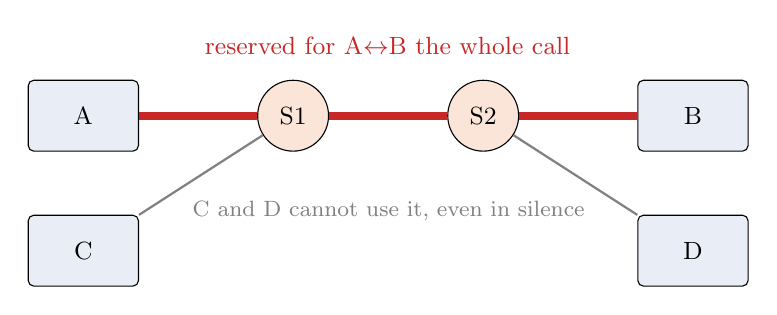
\begin{tikzpicture}
  \node[host] (a) {A};
  \node[rtr,right=15mm of a] (s1) {S1};
  \node[rtr,right=15mm of s1] (s2) {S2};
  \node[host,right=15mm of s2] (b) {B};
  \node[host,below=8mm of a] (c) {C};
  \node[host,below=8mm of b] (d) {D};
  \draw[line width=3pt,cnred] (a) -- (s1) -- (s2) -- (b);
  \draw[thick,gray] (c) -- (s1); \draw[thick,gray] (s2) -- (d);
  \node[above=2mm of s1,xshift=12mm,font=\small,cnred] {reserved for A$\leftrightarrow$B the whole call};
  \node[below=1mm of s2,xshift=-12mm,font=\footnotesize,gray,yshift=-4mm] {C and D cannot use it, even in silence};
\end{tikzpicture}
\end{center}

\begin{itemize}
  \item \textbf{Good --- guaranteed:} once set up, the full capacity is yours. Predictable, stable, no surprises mid-call.
  \item \textbf{Bad --- wasteful for bursty data:} go quiet for a few seconds and the reserved capacity sits idle, unusable by anyone else.
\end{itemize}

\section{Packet switching --- how the core really moves data}

\subsection{What exactly is a packet?}
\begin{itemize}
  \item Your message (a photo, a webpage, a voice clip) is chopped into small, independent chunks called \textbf{packets}.
  \item Each packet = \textbf{header} (addressing information) + \textbf{payload} (your actual data).
  \item Packets can take \textbf{different routes} to the same destination.
  \item The core forwards each packet independently, \textbf{hop by hop}, router to router.
\end{itemize}

\begin{center}
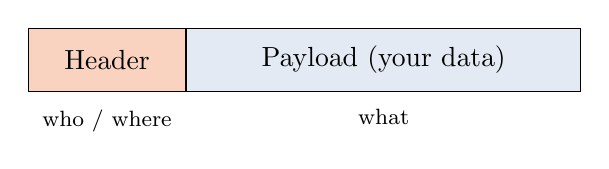
\begin{tikzpicture}
  \node[draw,fill=cnorange!25,minimum width=20mm,minimum height=8mm] (h) {Header};
  \node[draw,fill=cnblue!12,minimum width=50mm,minimum height=8mm,right=0mm of h] (p) {Payload (your data)};
  \node[below=1mm of h,font=\footnotesize] {who / where};
  \node[below=1mm of p,font=\footnotesize] {what};
\end{tikzpicture}
\end{center}

\subsection{The store-and-forward rule}
A router must \textbf{receive the entire packet} before it sends even the first bit onward: receive fully $\to$ check $\to$ forward fully.

\begin{center}
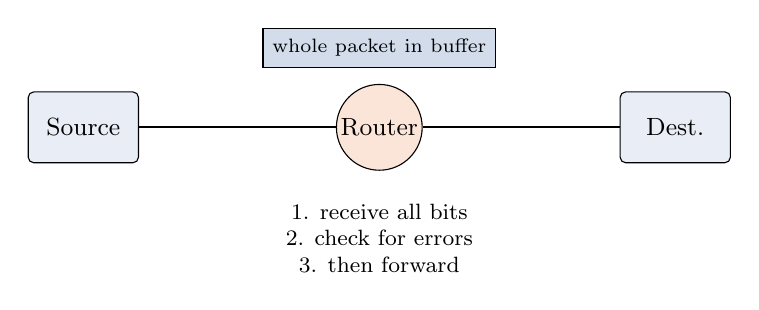
\begin{tikzpicture}
  \node[host] (s) {Source};
  \node[rtr,right=25mm of s] (r) {Router};
  \node[host,right=25mm of r] (d) {Dest.};
  \draw[thick] (s) -- (r) -- (d);
  \node[draw,fill=cnblue!20,minimum width=18mm,minimum height=5mm,above=2mm of r,font=\scriptsize] (buf) {whole packet in buffer};
  \node[below=3mm of r,font=\footnotesize,align=center] {1. receive all bits\\2. check for errors\\3. then forward};
\end{tikzpicture}
\end{center}

\textbf{Why it matters:} no single router needs to know the whole path. It only needs to know the \textbf{next hop}.

\section{Statistical multiplexing --- sharing on demand}

No reservations. Links are used only when packets actually need them. This one idea gives two ``superpowers'':

\begin{itemize}
  \item \textbf{Efficiency:} real traffic is \textbf{bursty} --- you are rarely sending every millisecond. Many users can share one link because it is statistically unlikely that they all burst at once.
  \item \textbf{Resilience:} packets are not tied to one fixed path. If a link or router fails, traffic is simply \textbf{rerouted} around the damage --- nothing was ``reserved'' there to lose.
\end{itemize}

\begin{center}
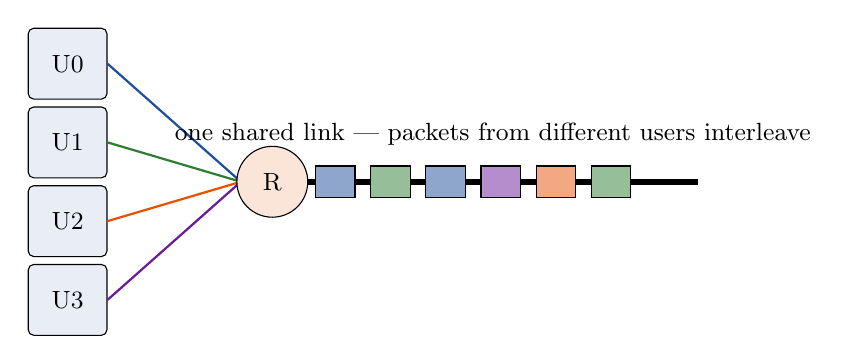
\begin{tikzpicture}
  \foreach \i/\c in {0/cnblue,1/cngreen,2/cnorange,3/cnpurple} {
    \node[host,minimum width=10mm] (u\i) at (0,-\i*1.0) {U\i};
    \draw[thick,\c] (u\i.east) -- (2.2,-1.5);
  }
  \node[rtr] (m) at (2.6,-1.5) {R};
  \draw[line width=2pt] (m) -- (8,-1.5);
  \foreach \x/\c in {3.4/cnblue,4.1/cngreen,4.8/cnblue,5.5/cnpurple,6.2/cnorange,6.9/cngreen} \node[draw,fill=\c!50,minimum width=5mm,minimum height=4mm] at (\x,-1.5) {};
  \node[font=\small,align=center] at (5.4,-0.9) {one shared link --- packets from different users interleave};
\end{tikzpicture}
\end{center}

\subsection{The catch: no guarantees}
Packet switching gives \textbf{no built-in guarantees}:
\begin{itemize}
  \item packets can be \textbf{delayed} behind others in a queue, or
  \item \textbf{dropped} entirely when a router's buffer fills up under load.
\end{itemize}

\begin{keyidea}[This is the seed of everything TCP does]
TCP (later lectures) exists to cover exactly this gap: it \textbf{detects loss, retransmits}, and \textbf{paces data}, so that an unreliable, best-effort core feels reliable to applications.
\end{keyidea}

\section{Sources of delay}

\subsection{The toll-booth caravan analogy}
Picture a caravan of cars arriving at a toll booth, then driving down a highway to the next toll booth. Each car passes the booth \textbf{one at a time} (fixed time each), then the cars drive the highway at the speed limit.

\begin{center}
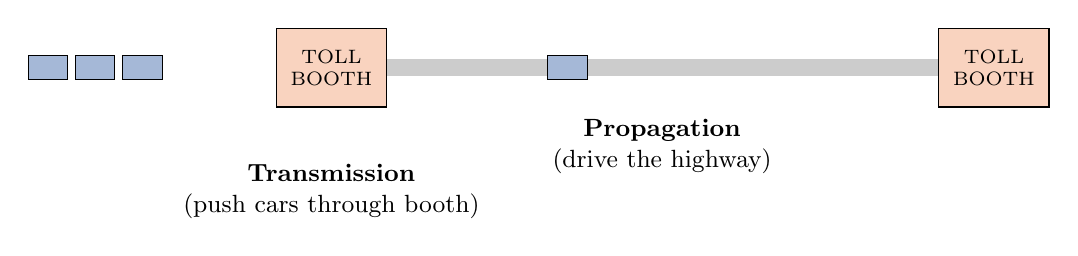
\begin{tikzpicture}
  \node[draw,fill=cnorange!25,minimum width=14mm,minimum height=10mm,align=center,font=\scriptsize] (t1) {TOLL\\BOOTH};
  \node[draw,fill=cnorange!25,minimum width=14mm,minimum height=10mm,align=center,font=\scriptsize,right=70mm of t1] (t2) {TOLL\\BOOTH};
  \draw[line width=6pt,gray!40] (t1.east) -- (t2.west);
  \foreach \x in {-3.6,-3.0,-2.4} \node[draw,fill=cnblue!40,minimum width=5mm,minimum height=3mm] at (\x,0) {};
  \node[draw,fill=cnblue!40,minimum width=5mm,minimum height=3mm] at (3.0,0) {};
  \node[below=6mm of t1,font=\small,align=center] {\textbf{Transmission}\\(push cars through booth)};
  \node[font=\small,align=center] at (4.2,-1.0) {\textbf{Propagation}\\(drive the highway)};
\end{tikzpicture}
\end{center}

\subsection{Every packet pays four kinds of delay}

\begin{center}
\begin{tabularx}{\textwidth}{>{\bfseries}l X l}
\toprule
Delay & What it is & Size / formula \\
\midrule
1. Processing & Router examines the header, checks for bit errors, decides where to send. & tiny, $\sim$ microseconds \\
2. Queuing & Time waiting in a buffer behind other packets. & variable (named only, not computed) \\
3. Transmission & Time to push \emph{all} the packet's bits onto the link. & $d_{trans} = L/R$ \\
4. Propagation & Time for one bit to physically travel along the link. & $d_{prop} = d/s$ \\
\bottomrule
\end{tabularx}
\end{center}

\[
d_{\text{nodal}} = d_{\text{proc}} + d_{\text{queue}} + d_{\text{trans}} + d_{\text{prop}}
\]

\subsection{Toll booth = transmission, highway = propagation}
\begin{center}
\begin{tabularx}{\textwidth}{X X}
\toprule
\textbf{Transmission delay (``toll-booth time'')} & \textbf{Propagation delay (``highway time'')} \\
\midrule
Time to push every car (every bit) through the booth before the last one can go. & Time actually driving between the two booths at a fixed speed limit. Has nothing to do with how many cars there are. \\
Depends on: \textbf{packet size} $L$ and \textbf{link rate} $R$. & Depends on: \textbf{distance} $d$ and \textbf{signal speed} $s$. \\
More booths (higher $R$) $\Rightarrow$ faster. & More lanes $\neq$ faster: you can't beat the speed limit. \\
\bottomrule
\end{tabularx}
\end{center}

\subsection{Transmission delay: $L/R$}
\[
d_{trans} = \frac{L \text{ (packet length in bits)}}{R \text{ (link rate in bits/sec)}}
\]
\begin{workedex}
$L = 8{,}000$ bits, $R = 2$ Mbps $= 2{,}000{,}000$ bits/s.
\[ d_{trans} = \frac{8{,}000}{2{,}000{,}000} = 0.004 \text{ s} = 4 \text{ ms} \]
Doubling the link rate halves the delay:
\begin{center}
\begin{tabular}{ccc}
\toprule
2 Mbps & 4 Mbps & 8 Mbps \\
\midrule
4 ms & 2 ms & 1 ms \\
\bottomrule
\end{tabular}
\end{center}
\end{workedex}

\subsection{Propagation delay: $d/s$}
\[
d_{prop} = \frac{d \text{ (distance in m)}}{s \text{ (signal speed} \approx 2\times 10^8 \text{ m/s in fibre)}}
\]

\begin{workedex}[The 500 Mbps link that still feels slow]
A geostationary satellite link is advertised at 500 Mbps, but video calls still have an awkward $\sim$half-second lag.

The satellite orbits about \textbf{35{,}786 km} above the equator. The signal goes up and back down: $\approx 71{,}500$ km, at the speed of light ($3\times 10^8$ m/s):
\[ d_{prop} \approx \frac{71{,}572 \times 10^3}{3\times 10^8} \approx 0.24 \text{ s} = 240 \text{ ms} \]
That is about 240 ms one way (up and down) \textbf{from physics alone}; a reply needs the same again, so the conversation feels laggy. More bandwidth (bigger $R$) cannot fix this, because the problem is $d$, not $R$.
\end{workedex}

\begin{center}
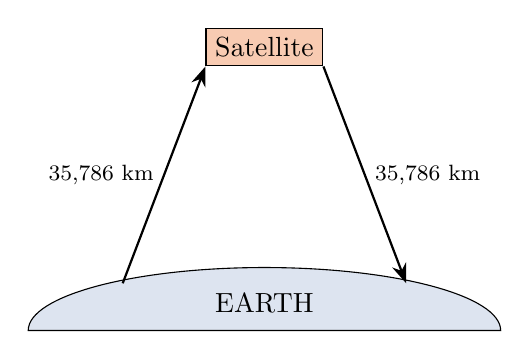
\begin{tikzpicture}
  \draw[fill=cnblue!15] (0,0) arc (180:0:3cm and 0.8cm) -- cycle;
  \node at (3,0.35) {EARTH};
  \node[draw,fill=cnorange!30,minimum width=10mm] (sat) at (3,3.6) {Satellite};
  \draw[arr] (1.2,0.6) -- node[left,font=\footnotesize]{35{,}786 km} (sat.south west);
  \draw[arr] (sat.south east) -- node[right,font=\footnotesize]{35{,}786 km} (4.8,0.6);
\end{tikzpicture}
\end{center}

\section{When packets don't make it}
If packets arrive at a router faster than it can send them out, they wait in the \textbf{queue (buffer)}. The buffer has limited size. When it is full, newly arriving packets are \textbf{dropped (lost)}. Lost packets must be re-sent by the previous node, the source, or not at all.

\begin{center}
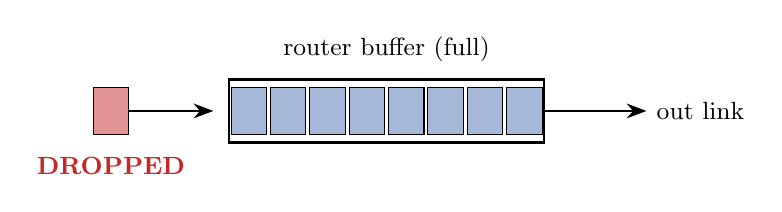
\begin{tikzpicture}
  \draw[thick] (0,0) rectangle (4,0.8);
  \foreach \x in {0,0.5,...,3.5} \node[draw,fill=cnblue!40,minimum width=4.5mm,minimum height=6mm] at (\x+0.25,0.4) {};
  \node[above=1mm,font=\small] at (2,0.8) {router buffer (full)};
  \node[draw,fill=cnred!50,minimum width=4.5mm,minimum height=6mm] (new) at (-1.5,0.4) {};
  \draw[arr] (new) -- (-0.2,0.4);
  \node[cnred,font=\small\bfseries] at (-1.5,-0.3) {DROPPED};
  \draw[arr] (4,0.4) -- (5.3,0.4) node[right,font=\small] {out link};
\end{tikzpicture}
\end{center}

\section{Throughput --- what you actually get}
\begin{itemize}
  \item \textbf{Throughput:} the rate (bits/sec) at which data is \emph{actually received} --- not the advertised or theoretical rate. ``What lands.''
  \item \textbf{Bottleneck link:} end-to-end throughput $\approx$ the \textbf{minimum} link rate on the path. The slowest hop sets the pace for everyone.
\end{itemize}
\[ \text{Throughput} \approx \min(R_1, R_2, \ldots, R_n) \]

\begin{center}
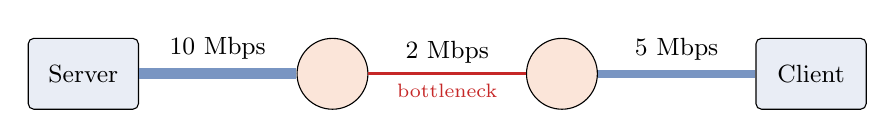
\begin{tikzpicture}
  \node[host] (s) {Server};
  \node[rtr,right=20mm of s] (r1) {};
  \node[rtr,right=20mm of r1] (r2) {};
  \node[host,right=20mm of r2] (c) {Client};
  \draw[line width=4pt,cnblue!60] (s) -- node[above,font=\small,text=black]{10 Mbps} (r1);
  \draw[line width=1pt,cnred] (r1) -- node[above,font=\small,text=black]{2 Mbps} node[below,font=\scriptsize,cnred]{bottleneck} (r2);
  \draw[line width=3pt,cnblue!60] (r2) -- node[above,font=\small,text=black]{5 Mbps} (c);
\end{tikzpicture}
\end{center}
End-to-end throughput here = \textbf{2 Mbps}, no matter how fast the other links are.

\begin{workedex}[``I pay for 300 Mbps. Why is it buffering?'']
Path: Netflix server $\to$ congested inter-network link $\to$ your ISP $\to$ home WiFi $\to$ your TV.
The 300 Mbps is only your \textbf{access link} to the ISP --- one stop on a long path. The real bottleneck could be a congested link between networks, an overloaded Netflix server, or (very often) your own \textbf{home WiFi} struggling with walls and interference. Ask: \emph{which hop is the slowest?}
\end{workedex}

\section{Looking ahead}
The core moves packets --- but thousands of different networks and apps must agree on a \textbf{format and order of operations}. That is the job of \textbf{protocol layers} (Lecture 3: OSI and TCP/IP models).

\begin{recap}
\begin{itemize}
  \item Circuit switching = reserved path, guaranteed but wasteful when idle. Packet switching = share on demand, efficient but no guarantees.
  \item Packet = header + payload. Routers use \textbf{store-and-forward}: receive whole packet, check, forward.
  \item Statistical multiplexing $\Rightarrow$ efficiency (bursty users share) + resilience (reroute around failure).
  \item Four delays: processing (tiny), queuing (variable), transmission $L/R$, propagation $d/s$.
  \item $L=8000$ bits, $R=2$ Mbps $\Rightarrow$ 4 ms. GEO satellite $\approx$ 240 ms propagation.
  \item Full buffer $\Rightarrow$ packet loss. Throughput = min link rate on path (bottleneck).
\end{itemize}
\end{recap}

\chapter{Lecture 3 --- OSI and TCP/IP Models}

\begin{keyidea}[The one idea from this lecture]
A network is far too complicated to design, build or debug as one single thing. \textbf{Layering} makes it manageable: each layer does \textbf{one job}, talks only to the layer directly above and below it, and deliberately knows nothing about the rest. Every later topic in this course sits inside one of these layers.
\end{keyidea}

\section{Where we left off}
\begin{center}
\begin{tabularx}{\textwidth}{>{\bfseries}l X}
\toprule
From Lecture 2 & What it said \\
\midrule
Packet $>$ circuit switching & Data is split into chunks that share links dynamically; far better for bursty traffic. \\
Store-and-forward & Routers fully receive, check and buffer a packet before forwarding it. \\
Anatomy of delay & Processing + queuing + transmission + propagation. \\
Throughput \& bottlenecks & Your speed is capped by the slowest link on the path, not your ISP plan. \\
\bottomrule
\end{tabularx}
\end{center}
The open question: thousands of networks, devices, operating systems and apps --- built by companies that never spoke to each other --- somehow \textbf{agree on the format} of packets and the \textbf{order of operations}. How? Answer: \textbf{layered models}.

\section{The idea behind layering}

\subsection{Sending a letter}
You write a letter, put it in an envelope and hand it to the postal service. Does the mail carrier care about the letter's contents? \textbf{No.}

That ``no'' is the whole idea:
\begin{itemize}
  \item The carrier needs only the \textbf{address on the envelope}.
  \item You need to know how to write a letter, nothing about sorting offices, vans or flights.
  \item Neither needs to understand the other's job --- and the letter still arrives.
\end{itemize}

\begin{analogy}[And what if the carrier \emph{does} care?]
If the carrier reads the letter, the separation breaks: your \textbf{privacy} is gone, and the carrier must now understand every kind of message anyone might send. A layer that looks inside the layer above stops being a clean layer. This is the seed of two later topics: \textbf{encryption} (making contents unreadable to the carrier) and \textbf{which devices may look how deep} into your traffic (see firewalls, Lecture 4).
\end{analogy}

\subsection{What layering buys us}
\begin{enumerate}
  \item Each layer solves \textbf{one problem} and can be understood on its own.
  \item A layer can be \textbf{replaced} without disturbing the others --- swap WiFi for Ethernet and nothing above needs rewriting.
  \item Different \textbf{vendors} can build different layers and still interoperate, because the boundaries are agreed in advance.
  \item When something breaks, you can \textbf{localise the fault} to one layer.
\end{enumerate}

\section{Encapsulation}

\subsection{The nesting doll}
\begin{itemize}
  \item \textbf{Going down} the sender's stack: each layer \textbf{wraps} the data from above with its own \textbf{header} (encapsulation).
  \item \textbf{Coming up} the receiver's stack: each layer \textbf{strips off} its own header and passes the rest up (decapsulation).
  \item \textbf{Symmetry:} layer 3 at the receiver reads exactly the header written by layer 3 at the sender. Each layer has a ``private conversation'' with its partner (peer) at the other end.
\end{itemize}

\begin{center}
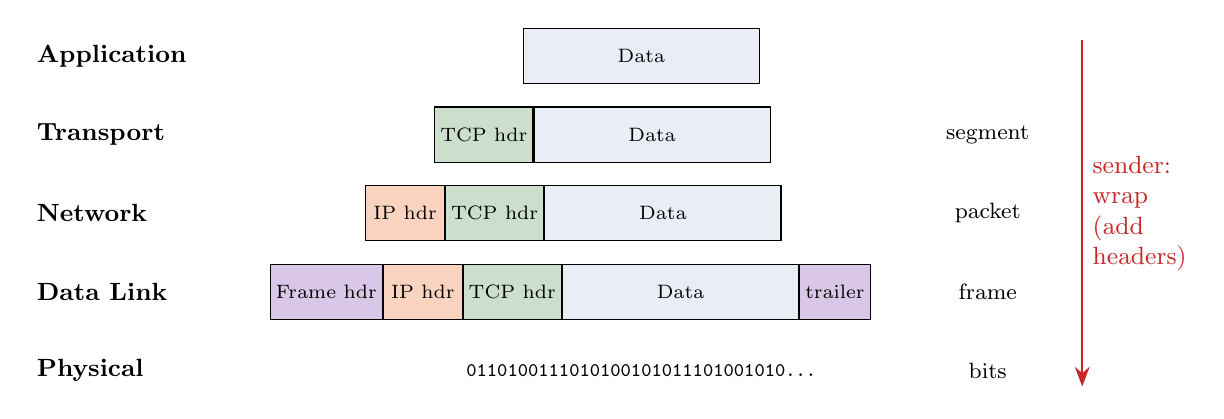
\begin{tikzpicture}[f/.style={draw,minimum height=7mm,font=\scriptsize,inner sep=2pt}]
  % data
  \node[f,fill=cnblue!10,minimum width=30mm] (d4) at (0,0) {Data};
  \node[font=\small\bfseries,anchor=west] at (-7.8,0) {Application};
  \node[f,fill=cngreen!25,minimum width=10mm] (t) at (-2,-1) {TCP hdr};
  \node[f,fill=cnblue!10,minimum width=30mm,right=0mm of t] {Data};
  \node[font=\small\bfseries,anchor=west] at (-7.8,-1) {Transport};
  \node[font=\footnotesize] at (4.4,-1) {segment};
  \node[f,fill=cnorange!25,minimum width=10mm] (ip) at (-3,-2) {IP hdr};
  \node[f,fill=cngreen!25,minimum width=10mm,right=0mm of ip] (t2) {TCP hdr};
  \node[f,fill=cnblue!10,minimum width=30mm,right=0mm of t2] {Data};
  \node[font=\small\bfseries,anchor=west] at (-7.8,-2) {Network};
  \node[font=\footnotesize] at (4.4,-2) {packet};
  \node[f,fill=cnpurple!25,minimum width=10mm] (eh) at (-4,-3) {Frame hdr};
  \node[f,fill=cnorange!25,minimum width=10mm,right=0mm of eh] (ip3) {IP hdr};
  \node[f,fill=cngreen!25,minimum width=10mm,right=0mm of ip3] (t3) {TCP hdr};
  \node[f,fill=cnblue!10,minimum width=30mm,right=0mm of t3] (d3) {Data};
  \node[f,fill=cnpurple!25,minimum width=8mm,right=0mm of d3] {trailer};
  \node[font=\small\bfseries,anchor=west] at (-7.8,-3) {Data Link};
  \node[font=\footnotesize] at (4.4,-3) {frame};
  \node[font=\small\bfseries,anchor=west] at (-7.8,-4) {Physical};
  \node[font=\scriptsize\ttfamily] at (0,-4) {0110100111010100101011101001010\ldots};
  \node[font=\footnotesize] at (4.4,-4) {bits};
  \draw[arr,cnred] (5.6,0.2) -- node[right,font=\small,align=left]{sender:\\wrap\\(add\\headers)} (5.6,-4.2);
\end{tikzpicture}
\end{center}

\subsection{The gift-wrapping version}
You wrap a gift in layers --- paper, then a box, then ribbon. The receiver unwraps in \textbf{exactly the reverse order}. You cannot untie the ribbon last.

\begin{examtip}
Encapsulation is what makes layering \emph{real}. A packet captured off a real network (e.g.\ in Wireshark) looks like a series of nested headers followed, finally, by your actual data. Reading a capture = peeling these layers.
\end{examtip}

\section{The OSI model}

\subsection{What it is}
\begin{itemize}
  \item \textbf{OSI} = \textbf{Open Systems Interconnection}.
  \item Divides network communication into \textbf{seven layers}, to simplify designing and reasoning about it.
  \item Developed by the \textbf{ISO} (International Organization for Standardization).
\end{itemize}

\subsection{Why learn it?}
\begin{itemize}
  \item \textbf{Everything you use runs on it} --- WhatsApp, games, Netflix. Learn it once and the internet stops being magic.
  \item \textbf{One map for a messy problem:} splits ``send data across the world'' into seven clean layers.
  \item \textbf{The industry's shared language:} ``that's a Layer 4 issue'' --- you'll understand and use this in interviews and debugging.
  \item \textbf{Foundation for everything after:} cybersecurity, cloud, AI infrastructure, backend engineering.
\end{itemize}

\subsection{Importance}
It provides a \textbf{standard} for network communication and ensures \textbf{interoperability} --- machines built by companies that never coordinated can still talk.

\begin{examtip}[Memory aid]
\textbf{Bottom-up (1 $\to$ 7):} \textbf{P}lease \textbf{D}o \textbf{N}ot \textbf{T}hrow \textbf{S}ausage \textbf{P}izza \textbf{A}way --- Physical, Data Link, Network, Transport, Session, Presentation, Application.\\[2pt]
\textbf{Top-down (7 $\to$ 1):} \textbf{A}ll \textbf{P}eople \textbf{S}eem \textbf{T}o \textbf{N}eed \textbf{D}ata \textbf{P}rocessing.\\[2pt]
Learn the \textbf{numbers} too: people say ``Layer 3'' far more often than ``Network layer''.
\end{examtip}

\begin{center}
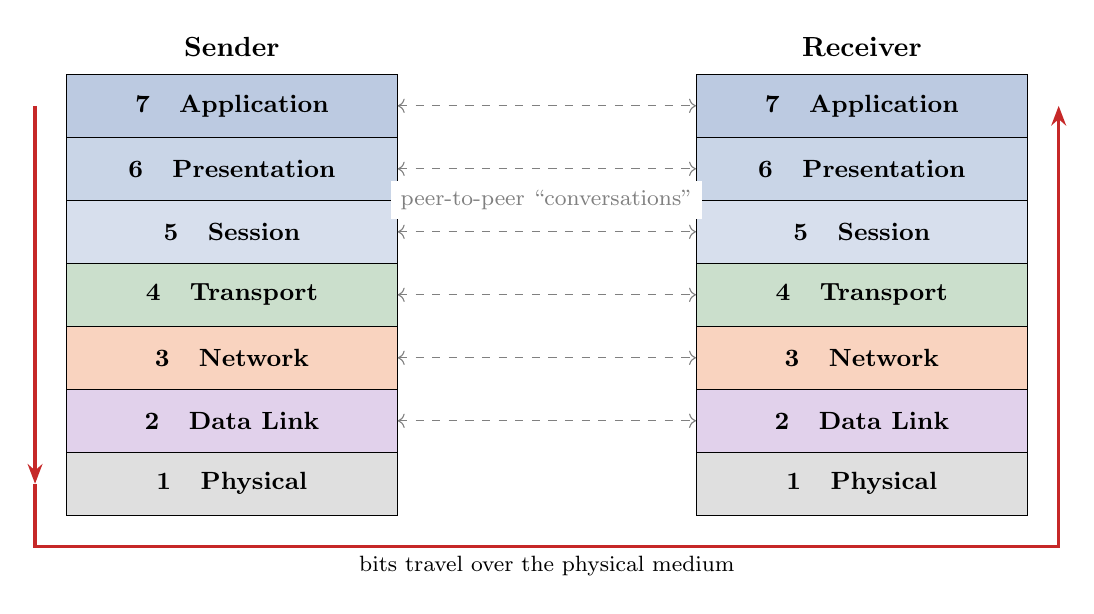
\begin{tikzpicture}[L/.style={draw,minimum width=42mm,minimum height=8mm,font=\small\bfseries}]
  \foreach \n/\name/\c [count=\i] in {7/Application/cnblue!30,6/Presentation/cnblue!24,5/Session/cnblue!18,4/Transport/cngreen!25,3/Network/cnorange!25,2/Data Link/cnpurple!20,1/Physical/gray!25} {
    \node[L,fill=\c] (s\n) at (0,-\i*0.8) {\n \quad \name};
    \node[L,fill=\c] (r\n) at (8,-\i*0.8) {\n \quad \name};
  }
  \node[above=1mm of s7,font=\bfseries] {Sender};
  \node[above=1mm of r7,font=\bfseries] {Receiver};
  \draw[arr,cnred,line width=1.2pt] (-2.5,-0.8) -- (-2.5,-5.6);
  \draw[arr,cnred,line width=1.2pt] (-2.5,-5.6) -- (-2.5,-6.4) -- (10.5,-6.4) -- (10.5,-0.8);
  \node[font=\footnotesize,below] at (4,-6.4) {bits travel over the physical medium};
  \foreach \n in {7,6,5,4,3,2} \draw[dashed,gray,<->] (s\n.east) -- (r\n.west);
  \node[font=\footnotesize,gray,fill=white] at (4,-2.0) {peer-to-peer ``conversations''};
\end{tikzpicture}
\end{center}

\section{The seven layers, one at a time}

\subsection{Layer 7 --- Application}
\textbf{Job:} delivers network services directly to end users; supports apps such as web browsers, email and file transfer. Unit: \textbf{data}.
\begin{analogy}[A waiter]
The waiter takes your order (user request), relays it to the kitchen (the network), and brings back your food (data). The customer never enters the kitchen; the chef never talks to the customer.
\end{analogy}

\subsection{Layer 6 --- Presentation}
\textbf{Job:} formats, encrypts and compresses data so it is readable and secure for the receiving app. Two headline jobs: \textbf{translation} and \textbf{encryption}.
\begin{itemize}
  \item ASCII $\leftrightarrow$ Unicode and other character-encoding conversions.
  \item Compression / decompression (zip, unzip).
  \item Encryption / decryption.
  \item Encoding images by type: PNG, JPEG, GIF.
\end{itemize}
\begin{analogy}[A translator]
Converts, formats and secures messages so sender and receiver understand each other even if they ``speak different languages''. Data must be presented the way the application wants it \emph{and} the way your system wants it.
\end{analogy}

\subsection{Layer 5 --- Session}
\textbf{Job:} establishes, manages and terminates \textbf{sessions} between two devices. Two named responsibilities: \textbf{dialog control} (whose turn is it?) and \textbf{synchronization}.
\begin{analogy}[A judge / panel moderator]
The judge calls ``Order! Order!'' and keeps proceedings running. A moderator starts the call, keeps it running smoothly and ends it when everyone is done.
\end{analogy}

\subsection{Layer 4 --- Transport}
\textbf{Job:} reliable, efficient delivery of data between two devices. Data is given source/destination addressing (ports), broken up for transit, and reassembled at the receiver.
\begin{analogy}[Many calls on one phone line]
Many separate conversations share one line. \textbf{Multiplexing} ensures each message reaches the right recipient.
\end{analogy}
\textbf{Link back to Lecture 2:} TCP lives here. Loss detection, retransmission and pacing are all Layer 4 jobs.

\subsection{Layer 3 --- Network}
\textbf{Job:} \textbf{logical addressing} (IP addresses) and \textbf{forwarding/routing} packets \textbf{across different networks}. Plainly: get packets from A to B.
\begin{analogy}[GPS]
A GPS finds the best route for delivery trucks (packets). Layer 3 doesn't care whether the next network is Ethernet, WiFi or fibre --- that indifference is what lets a ``network of networks'' exist.
\end{analogy}

\subsection{Layer 2 --- Data Link}
\textbf{Job:} reliable transfer between two \textbf{directly connected} nodes; \textbf{error detection} and \textbf{MAC addressing}. Scope: \textbf{one hop}, done correctly.
\begin{itemize}
  \item \textbf{Media access control --- ``one at a time!''} When many devices share a medium, something decides who transmits when.
  \item \textbf{Error checking:} detect whether the bits that arrived are the bits that were sent.
\end{itemize}
\begin{keyidea}[Layer 2 vs Layer 3 --- the most confused pair]
Layer 3 worries about the \textbf{whole journey} (end to end, across networks). Layer 2 worries only about getting safely to the \textbf{other end of one link}.
\end{keyidea}

\subsection{Layer 1 --- Physical}
\textbf{Job:} transmits \textbf{raw bits} (0s and 1s) over a physical medium: \textbf{coaxial cable}, \textbf{fibre optic cable}, \textbf{radio waves}.
\begin{analogy}[The roads and wires]
The roads, wires and signals the postman uses. No addresses, no routes, no meaning --- just moving something from here to there.
\end{analogy}
Propagation delay (Lecture 2) lives here: the speed of light in fibre is a Layer 1 fact that no protocol can argue with.

\subsection{The seven layers at a glance}
\begin{center}
\begin{tabularx}{\textwidth}{c l X l}
\toprule
\# & Layer & One-line job & Analogy \\
\midrule
7 & Application & Network services for users and their apps & The waiter \\
6 & Presentation & Translates, compresses, encrypts & The translator \\
5 & Session & Starts, maintains, ends the conversation & Judge / moderator \\
4 & Transport & Reliable, efficient delivery; multiplexing & Many calls on one line \\
3 & Network & Logical addressing and routing between networks & The GPS \\
2 & Data Link & Reliable transfer over one link; MAC; error checks & ``One at a time, please'' \\
1 & Physical & Moves raw bits over a medium & Roads and wires \\
\bottomrule
\end{tabularx}
\end{center}

\section{The TCP/IP model}

The TCP/IP model is a layered framework defining how data is transmitted over the internet, using standard protocols such as TCP and IP.

\textbf{Its status matters:} OSI is the model we use to \textbf{think and teach}. TCP/IP is the model the internet \textbf{actually runs on}. They are not really competitors --- one is a clean conceptual scheme, the other a working system that grew.

\begin{center}
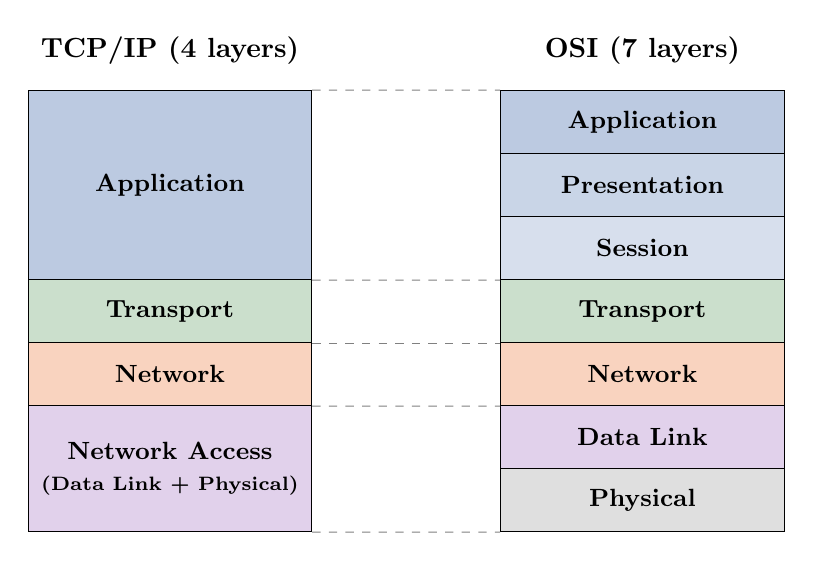
\begin{tikzpicture}[L/.style={draw,minimum width=36mm,font=\small\bfseries,align=center}]
  \node[L,fill=cnblue!30,minimum height=24mm] (a) at (0,0) {Application};
  \node[L,fill=cngreen!25,minimum height=8mm] (t) at (0,-1.6) {Transport};
  \node[L,fill=cnorange!25,minimum height=8mm] (n) at (0,-2.4) {Network};
  \node[L,fill=cnpurple!20,minimum height=16mm] (l) at (0,-3.6) {Network Access\\\scriptsize(Data Link + Physical)};
  % OSI right
  \begin{scope}[xshift=6cm]
  \foreach \name/\c [count=\i] in {Application/cnblue!30,Presentation/cnblue!24,Session/cnblue!18,Transport/cngreen!25,Network/cnorange!25,Data Link/cnpurple!20,Physical/gray!25}
    \node[L,fill=\c,minimum height=8mm] (o\i) at (0,1.6-\i*0.8) {\name};
  \end{scope}
  \node[above=2mm of a,font=\bfseries] {TCP/IP (4 layers)};
  \node[above=2mm of o1,font=\bfseries] {OSI (7 layers)};
  \draw[dashed,gray] (a.north east) -- (o1.north west); \draw[dashed,gray] (a.south east) -- (o3.south west);
  \draw[dashed,gray] (t.south east) -- (o4.south west);
  \draw[dashed,gray] (n.south east) -- (o5.south west);
  \draw[dashed,gray] (l.south east) -- (o7.south west);
\end{tikzpicture}
\end{center}

\subsection{OSI vs TCP/IP}
\begin{center}
\begin{tabularx}{\textwidth}{c X X}
\toprule
\# & OSI model & TCP/IP model \\
\midrule
1 & Open Systems Interconnection & Transmission Control Protocol / Internet Protocol \\
2 & 7 layers & 4 layers \\
3 & Developed by ISO (International Organization for Standardization) & Developed by DARPA (Defense Advanced Research Projects Agency) \\
4 & A conceptual model & Used in actual data transmission between computers \\
\bottomrule
\end{tabularx}
\end{center}

\begin{recap}
\begin{itemize}
  \item Layering: each layer one job; talks only to neighbours; can be replaced; faults can be localised.
  \item Encapsulation = add a header at each layer going down; decapsulation = strip it going up (nesting doll / gift wrap).
  \item OSI: 7 layers, by ISO. Mnemonic: Please Do Not Throw Sausage Pizza Away (1$\to$7).
  \item L7 waiter, L6 translator, L5 judge, L4 multiplexing/TCP, L3 GPS/IP, L2 one hop/MAC/errors, L1 raw bits.
  \item TCP/IP: 4 layers, by DARPA; what the internet actually runs on.
\end{itemize}
\end{recap}

\chapter{Lecture 4 --- Networking Devices, Topologies and the Cloud Network}

\begin{keyidea}[The one idea from this lecture]
Every networking device is best described by \textbf{which layer it works at}, i.e.\ \textbf{how deep into the packet it is willing to look}. A hub looks at nothing, a switch looks at MAC addresses (L2), a router looks at IP addresses (L3), a firewall looks at IPs and ports (L3/L4). Then we decide how to \textbf{arrange} the devices (topology), and see that the cloud does the same thing in \textbf{software}.
\end{keyidea}

\section{Why do we need network devices?}

\subsection{Connecting everyone directly does not scale}
If every computer gets its own cable to every other computer (a full mesh), the number of cables for $n$ devices is:
\[ \text{cables} = \frac{n(n-1)}{2} \]

\begin{center}
\begin{tabular}{rlr}
\toprule
Devices & Calculation & Cables needed \\
\midrule
3 & $3\times 2/2$ & 3 \\
10 & $10\times 9/2$ & 45 \\
100 & $100\times 99/2$ & 4{,}950 \\
1{,}000 & $1000\times 999/2$ & 499{,}500 \\
\bottomrule
\end{tabular}
\end{center}
Devices grow \textbf{linearly}, cables grow with the \textbf{square}. Ten times the devices $\approx$ a hundred times the cabling. Impossible for an office, let alone a data centre.

\subsection{The pivot: everyone connects to ONE device}
\begin{center}
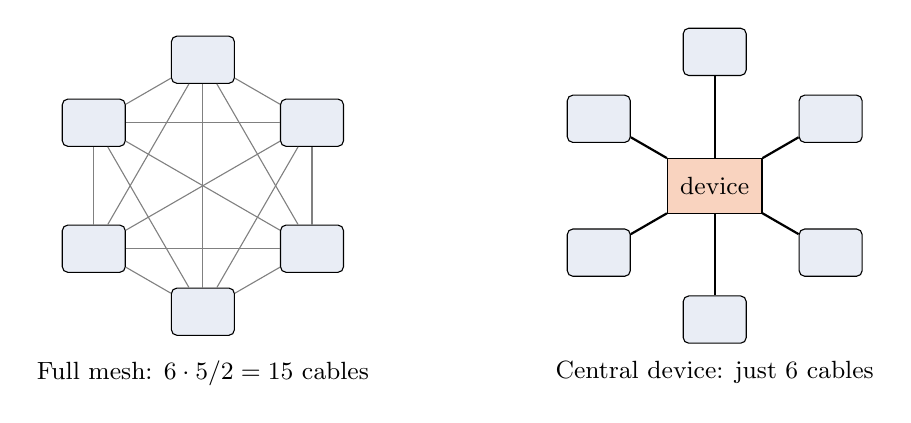
\begin{tikzpicture}
  \begin{scope}
    \foreach \a [count=\i] in {90,150,210,270,330,30} \node[host,minimum width=8mm,minimum height=6mm] (m\i) at (\a:1.6) {};
    \foreach \i in {1,...,6} \foreach \j in {1,...,6} { \ifnum\i<\j \draw[gray] (m\i) -- (m\j); \fi }
    \node[below=1mm,font=\small] at (0,-2.0) {Full mesh: $6\cdot5/2=15$ cables};
  \end{scope}
  \begin{scope}[xshift=6.5cm]
    \node[draw,fill=cnorange!25,minimum width=12mm,minimum height=7mm,font=\small] (c) at (0,0) {device};
    \foreach \a [count=\i] in {90,150,210,270,330,30} { \node[host,minimum width=8mm,minimum height=6mm] (s\i) at (\a:1.7) {}; \draw[thick] (c) -- (s\i); }
    \node[below=1mm,font=\small] at (0,-2.0) {Central device: just 6 cables};
  \end{scope}
\end{tikzpicture}
\end{center}
Now $n$ devices need only $n$ cables. \textbf{This single move is why networking hardware exists.} The rest of the lecture asks: what should that central device actually be?

\section{Networking devices}
Core components that connect computers and other devices: \textbf{hub, switch, wireless router, access point}, plus \textbf{firewall} and \textbf{load balancer}.

\subsection{The hub --- the 1980s answer (Layer 1)}
\begin{itemize}
  \item \textbf{Broadcasts} incoming data to \textbf{all} connected devices.
  \item Does \textbf{not} recognise hardware (MAC) addresses at all.
  \item Works at the \textbf{Physical layer (L1)}: takes the electrical signal on one port and repeats it out of every other port.
\end{itemize}

\begin{center}
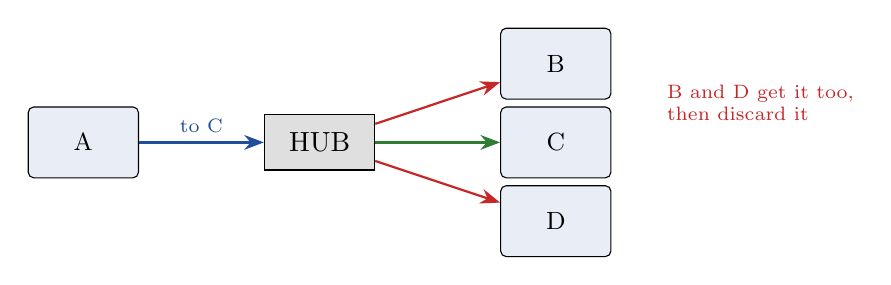
\begin{tikzpicture}
  \node[draw,fill=gray!25,minimum width=14mm,minimum height=7mm] (h) at (0,0) {HUB};
  \node[host] (a) at (-3,0) {A};
  \node[host] (b) at (3,1) {B};
  \node[host] (c) at (3,0) {C};
  \node[host] (d) at (3,-1) {D};
  \draw[arr,cnblue] (a) -- node[above,font=\scriptsize]{to C} (h);
  \draw[arr,cnred] (h) -- (b); \draw[arr,cngreen] (h) -- (c); \draw[arr,cnred] (h) -- (d);
  \node[font=\scriptsize,cnred,align=left] at (5.6,0.5) {B and D get it too,\\then discard it};
\end{tikzpicture}
\end{center}

\begin{examtip}[Class question: main real-world problem with a hub?]
\textbf{Unnecessary traffic.} Data goes to every device even when only one needs it. Every machine must receive, inspect and throw away traffic not meant for it, and while that traffic occupies the shared medium, nobody else can transmit. More devices $\Rightarrow$ worse congestion.
\end{examtip}

\subsection{The switch --- the 1990s answer (Layer 2)}
\begin{itemize}
  \item Works at the \textbf{Data Link layer (L2)}.
  \item Connects devices within a \textbf{LAN} and forwards data to the \textbf{correct} device using \textbf{MAC addresses}.
  \item Has \textbf{no understanding of Layer 3} --- IP addresses mean nothing to it.
  \item Ports can be configured; broadcasting can be controlled because it knows which MAC sits on which port.
\end{itemize}
\textbf{``The switch is a hub with a memory.''} It learns which MAC address lives behind which port (its MAC table), so it sends each frame only where it needs to go.

\begin{center}
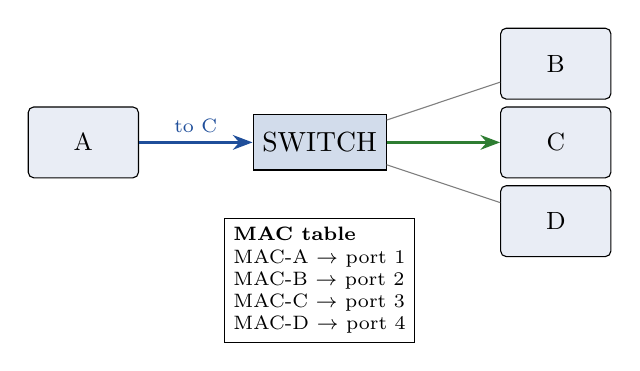
\begin{tikzpicture}
  \node[draw,fill=cnblue!20,minimum width=16mm,minimum height=7mm] (s) at (0,0) {SWITCH};
  \node[host] (a) at (-3,0) {A};
  \node[host] (b) at (3,1) {B};
  \node[host] (c) at (3,0) {C};
  \node[host] (d) at (3,-1) {D};
  \draw[arr,cnblue] (a) -- node[above,font=\scriptsize]{to C} (s);
  \draw[gray] (s) -- (b); \draw[arr,cngreen] (s) -- (c); \draw[gray] (s) -- (d);
  \node[draw,font=\scriptsize,below=6mm of s,align=left] {\textbf{MAC table}\\MAC-A $\to$ port 1\\MAC-B $\to$ port 2\\MAC-C $\to$ port 3\\MAC-D $\to$ port 4};
\end{tikzpicture}
\end{center}

\subsection{Hub vs switch}
\begin{center}
\begin{tabularx}{\textwidth}{>{\bfseries}l X X}
\toprule
 & Hub & Switch \\
\midrule
Era & 1980s & 1990s onward \\
Layer & L1 --- Physical & L2 --- Data Link \\
Addresses understood & None & MAC addresses \\
Forwarding & Broadcasts to every port & Sends to the correct port only \\
Main weakness & Unnecessary traffic; congestion grows with devices & Cannot see IP, so cannot reach another network \\
\bottomrule
\end{tabularx}
\end{center}

\subsection{The router --- reaching another network (Layer 3)}
A switch solves communication \emph{inside} one network. \textbf{What if we want to talk to a computer in another network?} The switch can't help (no L3 knowledge). The \textbf{router} can:
\begin{itemize}
  \item Routes data \textbf{between different networks}.
  \item Works at the \textbf{Network layer (L3)} using \textbf{IP addresses}. (The GPS from Lecture 3.)
\end{itemize}

\begin{center}
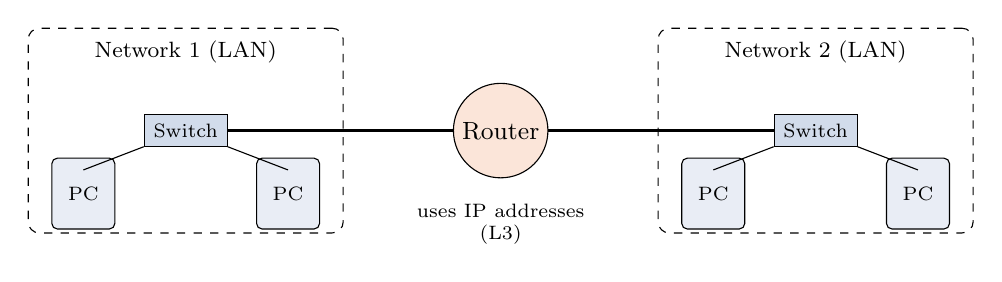
\begin{tikzpicture}
  \node[draw,dashed,rounded corners,minimum width=40mm,minimum height=26mm] (n1) at (0,0) {};
  \node[font=\footnotesize] at (0,1.0) {Network 1 (LAN)};
  \node[draw,fill=cnblue!20,font=\scriptsize] (s1) at (0,0) {Switch};
  \node[host,minimum width=8mm,font=\scriptsize] at (-1.3,-0.8) {PC}; \node[host,minimum width=8mm,font=\scriptsize] at (1.3,-0.8) {PC};
  \draw (s1) -- (-1.3,-0.5); \draw (s1) -- (1.3,-0.5);
  \node[draw,dashed,rounded corners,minimum width=40mm,minimum height=26mm] (n2) at (8,0) {};
  \node[font=\footnotesize] at (8,1.0) {Network 2 (LAN)};
  \node[draw,fill=cnblue!20,font=\scriptsize] (s2) at (8,0) {Switch};
  \node[host,minimum width=8mm,font=\scriptsize] at (6.7,-0.8) {PC}; \node[host,minimum width=8mm,font=\scriptsize] at (9.3,-0.8) {PC};
  \draw (s2) -- (6.7,-0.5); \draw (s2) -- (9.3,-0.5);
  \node[rtr,minimum size=12mm] (r) at (4,0) {Router};
  \draw[thick] (s1) -- (r) -- (s2);
  \node[font=\scriptsize,below=2mm of r,align=center] {uses IP addresses\\(L3)};
\end{tikzpicture}
\end{center}

\subsection{The firewall --- should every packet be allowed in?}
A router knows \emph{where} to send packets. But that raises a \textbf{security} question: should every packet be allowed to enter?
\begin{itemize}
  \item A \textbf{firewall} is a network security device.
  \item It \textbf{monitors} data coming into and going out of the network.
  \item Its main job: protect the network from unauthorised access or threats --- only authorised data gets through.
\end{itemize}

\textbf{Packet filtering.} A packet from outside passes the router, then the firewall inspects it:
\begin{center}
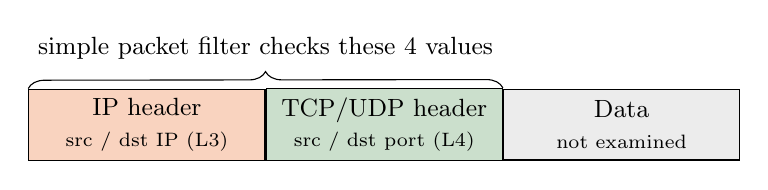
\begin{tikzpicture}
  \node[draw,fill=cnorange!25,minimum width=30mm,minimum height=9mm,align=center,font=\small] (ip) at (0,0) {IP header\\\scriptsize src / dst IP (L3)};
  \node[draw,fill=cngreen!25,minimum width=30mm,minimum height=9mm,align=center,font=\small,right=0mm of ip] (tcp) {TCP/UDP header\\\scriptsize src / dst port (L4)};
  \node[draw,fill=gray!15,minimum width=30mm,minimum height=9mm,align=center,font=\small,right=0mm of tcp] (d) {Data\\\scriptsize not examined};
  \draw[decorate,decoration={brace,amplitude=6pt}] (ip.north west) -- (tcp.north east) node[midway,above=7pt,font=\small] {simple packet filter checks these 4 values};
\end{tikzpicture}
\end{center}
So basic packet filtering decides on \textbf{four values}: source IP, destination IP, source port, destination port. IP is Layer 3, port is Layer 4 --- a packet-filtering firewall reads \textbf{two layers deep and stops}.

\begin{center}
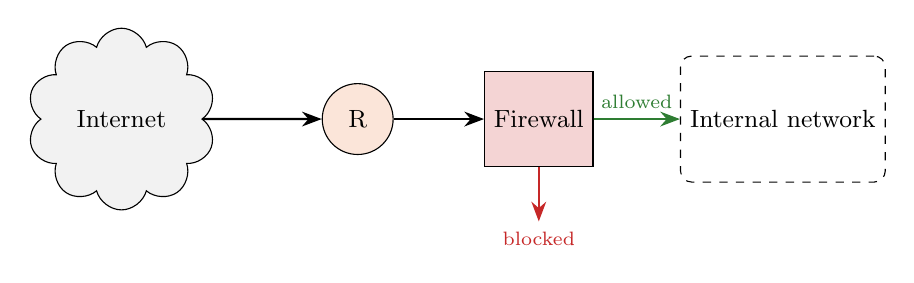
\begin{tikzpicture}
  \node[draw,cloud,cloud puffs=10,fill=gray!10,minimum width=24mm,minimum height=14mm,font=\small] (i) at (0,0) {Internet};
  \node[rtr] (r) at (3,0) {R};
  \node[draw,fill=cnred!20,minimum width=12mm,minimum height=12mm,font=\small] (f) at (5.3,0) {Firewall};
  \node[draw,dashed,rounded corners,minimum width=26mm,minimum height=16mm,font=\small] (lan) at (8.4,0) {Internal network};
  \draw[arr] (i) -- (r); \draw[arr] (r) -- (f); \draw[arr,cngreen] (f) -- node[above,font=\scriptsize]{allowed} (lan);
  \draw[arr,cnred] (f) -- ++(0,-1.3) node[below,font=\scriptsize]{blocked};
\end{tikzpicture}
\end{center}

\subsection{Load balancers}
A \textbf{load balancer} distributes incoming traffic across \textbf{multiple servers}, so no single server is overwhelmed. In class, six client requests were spread across three servers instead of piling onto one. Netflix, Google, Amazon and Facebook all rely on load balancers.

\begin{center}
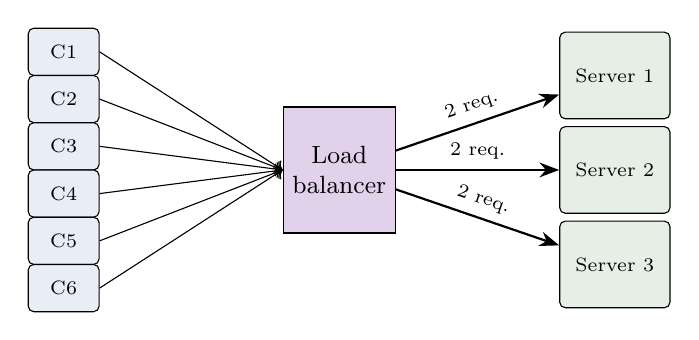
\begin{tikzpicture}
  \foreach \i in {1,...,6} \node[host,minimum width=9mm,minimum height=6mm,font=\scriptsize] (c\i) at (0,2.1-\i*0.6) {C\i};
  \node[draw,fill=cnpurple!20,minimum width=14mm,minimum height=16mm,align=center,font=\small] (lb) at (3.5,0) {Load\\balancer};
  \foreach \i in {1,...,6} \draw[->] (c\i.east) -- (lb.west);
  \foreach \i/\y in {1/1.2,2/0,3/-1.2} { \node[srv,font=\scriptsize] (s\i) at (7,\y) {Server \i}; \draw[arr] (lb) -- node[above,font=\scriptsize,sloped]{2 req.} (s\i); }
\end{tikzpicture}
\end{center}

\textbf{Link to Lecture 2:} it's the bottleneck idea again. When the slowest hop is a \emph{server} rather than a link, instead of making one server faster, you stop sending it everything.

\subsection{The devices by layer (memorise this!)}
\begin{center}
\begin{tabularx}{\textwidth}{>{\bfseries}l l X}
\toprule
Device & Layer & What it decides on \\
\midrule
Hub & L1 Physical & Nothing. Repeats signals to every port. \\
Switch & L2 Data Link & MAC addresses, within one LAN. \\
Router & L3 Network & IP addresses, between different networks. \\
Firewall & L3/L4 (and above) & IP addresses and port numbers; advanced types inspect more. \\
Load balancer & L4/L7 & Which of several servers should get this request. \\
Wireless router / access point & L1--L3 (by role) & Provide wireless access to the network. \\
\bottomrule
\end{tabularx}
\end{center}

\begin{center}
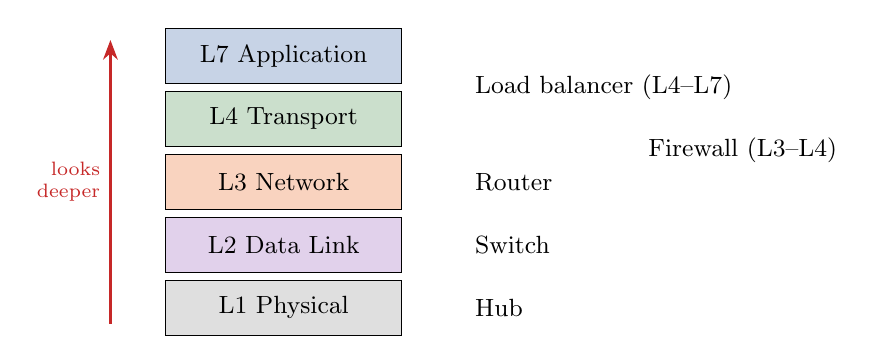
\begin{tikzpicture}[L/.style={draw,minimum width=30mm,minimum height=7mm,font=\small}]
  \node[L,fill=cnblue!25] (l7) at (0,0) {L7 Application};
  \node[L,fill=cngreen!25] (l4) at (0,-0.8) {L4 Transport};
  \node[L,fill=cnorange!25] (l3) at (0,-1.6) {L3 Network};
  \node[L,fill=cnpurple!20] (l2) at (0,-2.4) {L2 Data Link};
  \node[L,fill=gray!25] (l1) at (0,-3.2) {L1 Physical};
  \node[right=8mm of l1,font=\small] {Hub};
  \node[right=8mm of l2,font=\small] {Switch};
  \node[right=8mm of l3,font=\small] {Router};
  \node[right=30mm of l3,font=\small,yshift=4mm] {Firewall (L3--L4)};
  \node[right=8mm of l7,font=\small,yshift=-4mm] {Load balancer (L4--L7)};
  \draw[arr,cnred] (-2.2,-3.4) -- node[left,font=\scriptsize,align=right]{looks\\deeper} (-2.2,0.2);
\end{tikzpicture}
\end{center}

\section{Network topologies}
\textbf{Topology} = the arrangement of devices and their connections in a network, including how data flows. Types named: \textbf{star, mesh, hybrid, ring, bus}.

\begin{center}
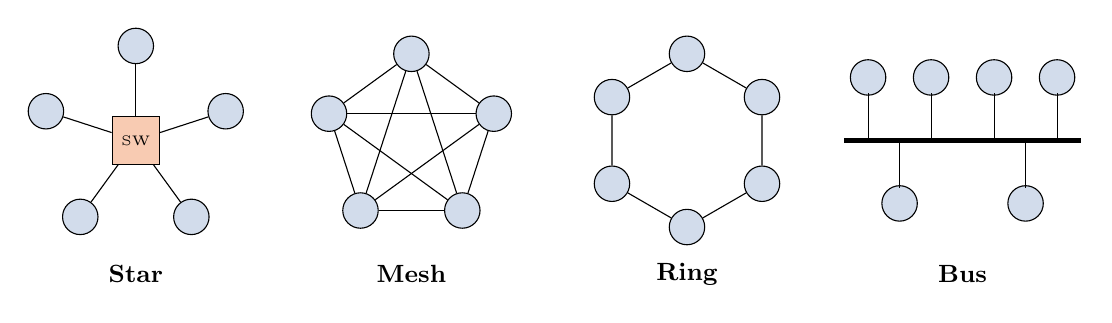
\begin{tikzpicture}[n/.style={draw,circle,fill=cnblue!20,minimum size=4.5mm,inner sep=0pt}]
  % star
  \begin{scope}
    \node[draw,fill=cnorange!30,minimum size=6mm,font=\tiny] (c) at (0,0) {SW};
    \foreach \a [count=\i] in {90,162,234,306,18} {\node[n] (s\i) at (\a:1.2) {}; \draw (c) -- (s\i);}
    \node[font=\small\bfseries] at (0,-1.7) {Star};
  \end{scope}
  % mesh
  \begin{scope}[xshift=3.5cm]
    \foreach \a [count=\i] in {90,162,234,306,18} \node[n] (m\i) at (\a:1.1) {};
    \foreach \i in {1,...,5} \foreach \j in {1,...,5} { \ifnum\i<\j \draw (m\i) -- (m\j); \fi }
    \node[font=\small\bfseries] at (0,-1.7) {Mesh};
  \end{scope}
  % ring
  \begin{scope}[xshift=7cm]
    \foreach \a [count=\i] in {90,150,210,270,330,30} \node[n] (r\i) at (\a:1.1) {};
    \draw (r1)--(r2)--(r3)--(r4)--(r5)--(r6)--(r1);
    \node[font=\small\bfseries] at (0,-1.7) {Ring};
  \end{scope}
  % bus
  \begin{scope}[xshift=10.5cm]
    \draw[line width=2pt] (-1.5,0) -- (1.5,0);
    \foreach \x in {-1.2,-0.4,0.4,1.2} {\node[n] at (\x,0.8) {}; \draw (\x,0) -- (\x,0.6);}
    \foreach \x in {-0.8,0.8} {\node[n] at (\x,-0.8) {}; \draw (\x,0) -- (\x,-0.6);}
    \node[font=\small\bfseries] at (0,-1.7) {Bus};
  \end{scope}
\end{tikzpicture}
\end{center}

\subsection{Star topology}
\begin{itemize}
  \item All devices connect to a \textbf{central hub or switch}.
  \item Data flows sender $\to$ hub/switch $\to$ receiver.
  \item Centralised structure makes diagnostics and maintenance easy --- one obvious place to look.
  \item Popular for \textbf{LANs}; stays manageable as it grows.
  \item \textbf{Weakness:} the central device is a \textbf{single point of failure}.
\end{itemize}

\subsection{Mesh topology}
\begin{itemize}
  \item Every device is \textbf{directly connected to all others}.
  \item Many possible paths between any two devices $\Rightarrow$ high reliability: if one path fails, use another.
  \item Cost: the $n(n-1)/2$ problem --- jokingly called ``\textbf{spaghetti networks}''.
  \item Very useful when links are \textbf{wireless}: wireless mesh networks extend WiFi coverage, because adding a node adds paths, not cables.
\end{itemize}

\subsection{Hybrid topology}
Combines two or more topologies (e.g.\ star + ring + bus segments) into a more complex, flexible network. Real large networks are almost always hybrids because different parts of an organisation have different needs.

\subsection{Ring and bus (named in class)}
\begin{itemize}
  \item \textbf{Ring:} each device connects to two neighbours, forming a circle; data travels around the ring.
  \item \textbf{Bus:} all devices share one main cable (the ``bus'').
\end{itemize}

\subsection{Choosing a topology by environment}
\begin{center}
\begin{tabularx}{\textwidth}{l l X l}
\toprule
Environment & Topology & Reason & Example devices \\
\midrule
Small office & Star & Easy setup, centralised control & Laptops, printers, routers \\
Smart home & Mesh & Reliable, direct device-to-device communication & Smart bulbs, cameras \\
Data centre & Hybrid & Combines benefits of multiple topologies & Servers, storage units \\
\bottomrule
\end{tabularx}
\end{center}

\subsection{Fault tolerance and scalability}
\begin{center}
\begin{tabular}{lll}
\toprule
Topology & Fault tolerance & Scalability \\
\midrule
Star & Medium & Good \\
Mesh & High & Excellent \\
Hybrid & High & Hard \\
\bottomrule
\end{tabular}
\end{center}
Read this as \textbf{trade-offs}, not a ranking. ``Which topology is best?'' is not a good question; ask ``best for what, at what size, at what cost?''

\section{Hardware meets software: the cloud network}

\subsection{The evolutionary shift}
Traditional networking = physical boxes, special cables, manual configuration. In the cloud, the \textbf{logic is the same} (same layers, devices, topologies) but everything is \textbf{software-defined}.
\begin{center}
\begin{tabular}{lcl}
\toprule
Traditional & & Cloud era \\
\midrule
Physical box & $\to$ & Virtual instance \\
Copper cables & $\to$ & Virtualised overlays \\
Manual wiring & $\to$ & API calls or console clicks \\
\bottomrule
\end{tabular}
\end{center}
Nothing you learned becomes obsolete: a load balancer in AWS is still a load balancer; a subnet still partitions a Layer 3 network.

\subsection{AWS foundation: regions and edge locations}
\begin{itemize}
  \item \textbf{Regions:} isolated geographic areas (e.g.\ Mumbai), each with multiple data-centre clusters. 30+ globally, linked by an ultra-low-latency backbone.
  \item \textbf{Edge locations:} CDN endpoints that \textbf{cache content closer to users} to reduce latency.
\end{itemize}
Edge locations = Lecture 2 made concrete: caching closer shortens $d$ in $d/s$, so propagation delay falls. Same reason Netflix puts appliances inside ISPs.

\subsection{Redundancy: Availability Zones (AZs)}
\begin{itemize}
  \item An \textbf{AZ} = one or more discrete data centres with redundant power, networking and connectivity --- an isolated \textbf{fault domain}.
  \item Deploy across \textbf{two or more AZs} so your app survives a fire, flood or power failure at any one site.
\end{itemize}

\subsection{The Virtual Private Cloud (VPC)}
\begin{itemize}
  \item A \textbf{VPC} is your own private, software-defined network inside AWS. You control IP ranges, subnets and routing (\textbf{logical isolation}).
  \item \textbf{Subnets map to specific AZs}, partitioning your L3 network for scale and security.
  \item Addresses are written in \textbf{CIDR notation} (e.g.\ \texttt{10.0.0.0/16}): you get a block of addresses and decide how to carve it up.
\end{itemize}

\begin{center}
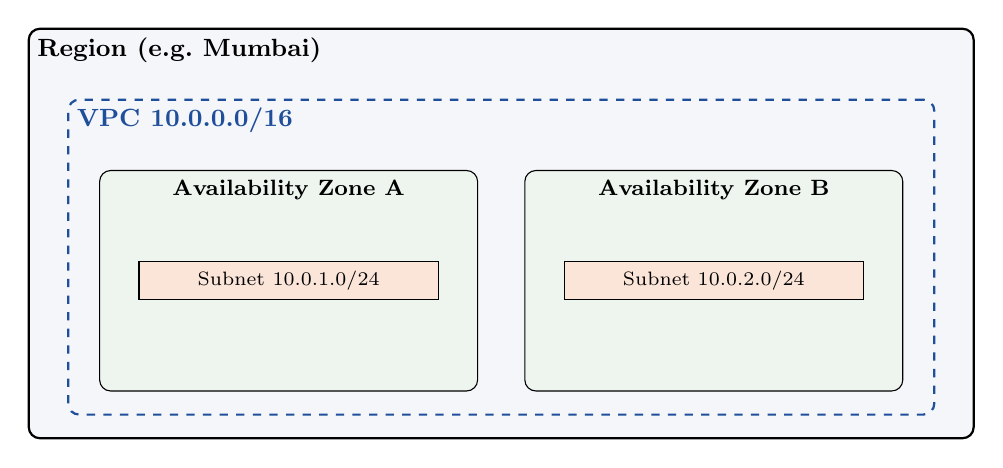
\begin{tikzpicture}
  \node[draw,thick,rounded corners,minimum width=120mm,minimum height=52mm,fill=cngrey] (reg) at (0,0) {};
  \node[anchor=north west,font=\small\bfseries] at (reg.north west) {Region (e.g.\ Mumbai)};
  \node[draw,thick,dashed,rounded corners,minimum width=110mm,minimum height=40mm,cnblue] (vpc) at (0,-0.3) {};
  \node[anchor=north west,font=\small\bfseries,cnblue] at (vpc.north west) {VPC  10.0.0.0/16};
  \node[draw,rounded corners,fill=cngreen!8,minimum width=48mm,minimum height=28mm] (az1) at (-2.7,-0.6) {};
  \node[anchor=north,font=\footnotesize\bfseries] at (az1.north) {Availability Zone A};
  \node[draw,fill=cnorange!15,font=\scriptsize,minimum width=38mm] at (-2.7,-0.6) {Subnet 10.0.1.0/24};
  \node[draw,rounded corners,fill=cngreen!8,minimum width=48mm,minimum height=28mm] (az2) at (2.7,-0.6) {};
  \node[anchor=north,font=\footnotesize\bfseries] at (az2.north) {Availability Zone B};
  \node[draw,fill=cnorange!15,font=\scriptsize,minimum width=38mm] at (2.7,-0.6) {Subnet 10.0.2.0/24};
\end{tikzpicture}
\end{center}

\begin{recap}
\begin{itemize}
  \item Full mesh needs $n(n-1)/2$ cables; a central device needs $n$.
  \item Hub = L1, broadcasts everything (unnecessary traffic). Switch = L2, MAC table, sends to correct port only. Router = L3, between networks.
  \item Firewall packet filter checks src/dst IP (L3) + src/dst port (L4), not data. Load balancer spreads requests over servers.
  \item Star (central, single point of failure), Mesh (reliable, costly ``spaghetti''), Hybrid (real world), Ring, Bus.
  \item Cloud = same ideas in software: Region, Edge location (CDN cache), AZ (fault domain), VPC (your private network), subnets per AZ, CIDR.
\end{itemize}
\end{recap}

\chapter{Lecture 5 --- Application Layer: Architecture, Protocols and APIs}

\begin{keyidea}[The one idea from this lecture]
The \textbf{application layer} is where programs (browsers, email apps) meet the network. Its most important protocol is \textbf{HTTP}: a simple, \textbf{stateless request--response} protocol. HTTP has evolved (1.0 $\to$ 1.1 $\to$ 2 $\to$ 3) mainly to fight one enemy: \textbf{head-of-line blocking}. Finally, apps talk to other apps through \textbf{APIs}, most commonly \textbf{REST} APIs.
\end{keyidea}

\textbf{Roadmap:} Network architectures $\cdot$ Application layer $\cdot$ HTTP $\cdot$ HTTP methods $\cdot$ Evolution of HTTP $\cdot$ Head-of-Line blocking $\cdot$ HTTP/2 and HTTP/3 $\cdot$ REST principles.

\section{Network architectures}

\begin{center}
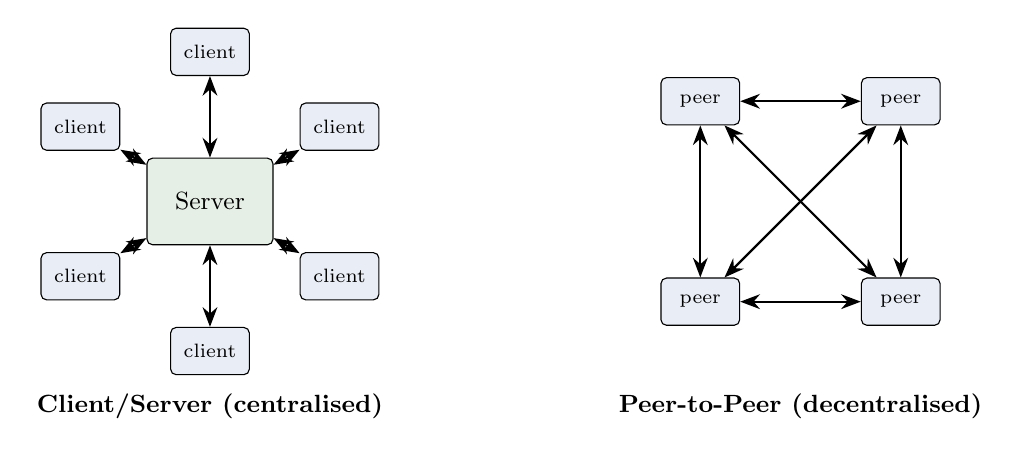
\begin{tikzpicture}
  \begin{scope}
    \node[srv,minimum width=16mm] (s) at (0,0) {Server};
    \foreach \a [count=\i] in {90,150,210,270,330,30} { \node[host,minimum width=10mm,minimum height=6mm,font=\scriptsize] (c\i) at (\a:1.9) {client}; \draw[darr] (c\i) -- (s); }
    \node[font=\small\bfseries] at (0,-2.6) {Client/Server (centralised)};
  \end{scope}
  \begin{scope}[xshift=7.5cm]
    \foreach \a [count=\i] in {45,135,225,315} \node[host,minimum width=10mm,minimum height=6mm,font=\scriptsize] (p\i) at (\a:1.8) {peer};
    \foreach \i in {1,...,4} \foreach \j in {1,...,4} { \ifnum\i<\j \draw[darr] (p\i) -- (p\j); \fi }
    \node[font=\small\bfseries] at (0,-2.6) {Peer-to-Peer (decentralised)};
  \end{scope}
\end{tikzpicture}
\end{center}

\begin{itemize}
  \item \textbf{Client/Server:} centralised. Powerful \textbf{servers} store data and process requests for many dependent \textbf{clients}. (Example: a browser and a web server.)
  \item \textbf{Peer-to-Peer (P2P):} decentralised. All devices (``peers'') act as \textbf{both clients and servers} with equal privileges. (Example: BitTorrent-style file sharing.)
\end{itemize}
Next question: \emph{how do these systems actually talk over the network?} A client sends a \textbf{request} over a \textbf{connection}, the server sends a \textbf{response}.

\section{The application layer}
\textbf{Recap:} in the 7-layer OSI stack the sender's data goes \textbf{down} the layers (Application $\to$ Physical), across the physical link, and \textbf{up} the receiver's layers. The application layer is at the very top.

The \textbf{Application Layer (Layer 7)} is the direct interface between software programs (web browsers, email clients) and the underlying network. It interprets user commands and enables data exchange across systems.

\textbf{Application layer protocols} (one for each kind of job):
\begin{center}
\begin{tabular}{ll}
\toprule
Job & Protocol \\
\midrule
Web surfing & HTTP / HTTPS \\
File transfer & FTP \\
Emails & SMTP (and POP3/IMAP --- Lecture 7) \\
Virtual terminals (remote login) & Telnet (and SSH) \\
Names $\to$ addresses & DNS (Lecture 8) \\
\bottomrule
\end{tabular}
\end{center}

\section{HTTP --- the web's language}

\textbf{HTTP (HyperText Transfer Protocol)} is a \textbf{stateless request--response} protocol (running over TCP).
\begin{itemize}
  \item The client (browser) sends a \textbf{REQUEST} to a server.
  \item The server processes it and sends back a \textbf{RESPONSE}.
  \item Each exchange is \textbf{independent} --- the server \textbf{remembers nothing} between requests (that's what \emph{stateless} means).
\end{itemize}

\begin{center}
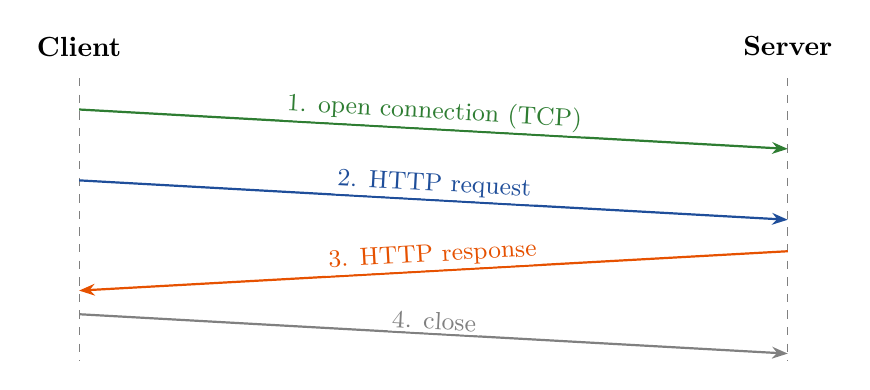
\begin{tikzpicture}
  \node[font=\bfseries] at (0,0.4) {Client}; \node[font=\bfseries] at (9,0.4) {Server};
  \lifelines{0}{9}{0}{-3.6}
  \draw[msg,cngreen] (0,-0.4) -- node[above,font=\small]{1. open connection (TCP)} (9,-0.9);
  \draw[msg,cnblue] (0,-1.3) -- node[above,font=\small]{2. HTTP request} (9,-1.8);
  \draw[msg,cnorange] (9,-2.2) -- node[above,font=\small]{3. HTTP response} (0,-2.7);
  \draw[msg,gray] (0,-3.0) -- node[above,font=\small]{4. close} (9,-3.5);
\end{tikzpicture}
\end{center}

\subsection{Structure of an HTTP message}
Both requests and responses have the same three-part shape:
\begin{center}
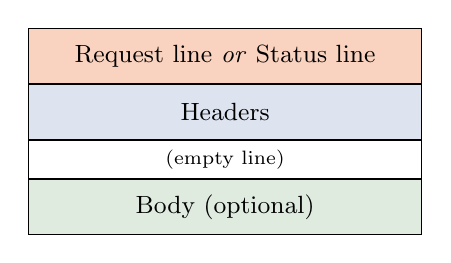
\begin{tikzpicture}[r/.style={draw,minimum width=50mm,minimum height=7mm,font=\small}]
  \node[r,fill=cnorange!25] (a) at (0,0) {Request line \emph{or} Status line};
  \node[r,fill=cnblue!15,below=0mm of a] (b) {Headers};
  \node[r,fill=white,below=0mm of b,minimum height=4mm,font=\scriptsize] (e) {(empty line)};
  \node[r,fill=cngreen!15,below=0mm of e] (c) {Body (optional)};
\end{tikzpicture}
\end{center}

\subsection{The HTTP request}
\begin{lstlisting}
GET /index.html HTTP/1.1          <- request line
Host: example.com                 <- headers
User-Agent: Chrome
Accept-Language: en-us
                                  <- empty line
(body: optional, e.g. form data or JSON for POST/PUT)
\end{lstlisting}

\textbf{1. Request line} --- three parts:
\begin{itemize}
  \item \textbf{Method:} the operation the client wants (GET, POST, PUT, DELETE, \ldots).
  \item \textbf{URL:} the resource/endpoint requested (e.g.\ \texttt{/index.html}, \texttt{/api/data}).
  \item \textbf{HTTP version:} e.g.\ \texttt{HTTP/1.1} or \texttt{HTTP/2}.
\end{itemize}

\textbf{2. Headers} --- extra information about the request or about the client's capabilities:
\begin{itemize}
  \item \texttt{User-Agent}: the client software (browser, app, \ldots).
  \item \texttt{Host}: the domain name of the server.
  \item \texttt{Content-Type}: type of data the client is sending (for POST/PUT).
  \item \texttt{Accept}: types of data the client can handle (e.g.\ \texttt{text/html}, \texttt{application/json}).
\end{itemize}

\textbf{3. Body (optional)} --- the actual data sent by the client (form data, JSON payload). Only for methods like \textbf{POST, PUT, PATCH}. Example:
\begin{lstlisting}
{ "username": "user1", "password": "password123" }
\end{lstlisting}

\subsection{HTTP methods overview}
\begin{center}
\begin{tabularx}{\textwidth}{>{\ttfamily\bfseries}l X l}
\toprule
\textrm{Method} & Meaning & Has body? \\
\midrule
GET & Read / fetch a resource & No \\
POST & Create something new / submit data & Yes \\
PUT & Replace / update a resource & Yes \\
PATCH & Partially update a resource & Yes \\
DELETE & Remove a resource & Usually no \\
HEAD & Like GET but only headers, no body & No \\
OPTIONS & Ask which methods the server supports & No \\
\bottomrule
\end{tabularx}
\end{center}
\textbf{Safe methods} (do not change server state): GET, HEAD, OPTIONS. POST/PUT/DELETE have \textbf{side effects}.

\subsection{The HTTP response}
\begin{lstlisting}
HTTP/1.1 200 OK                   <- status line
Content-Type: text/html           <- headers
Content-Length: 88
Server: Apache/2.4.2
                                  <- empty line
<html><body><h1>Welcome to Example.com</h1></body></html>   <- body
\end{lstlisting}

\textbf{1. Status line:} HTTP version + \textbf{status code} (3 digits) + \textbf{status message} (short text). Example: \texttt{HTTP/1.1 200 OK}.

\textbf{2. Headers} (metadata about the response):
\texttt{Content-Type} (type of body, e.g.\ \texttt{text/html}, \texttt{application/json}), \texttt{Content-Length} (body length in bytes), \texttt{Server} (server software), \texttt{Date} (when the response was sent).

\textbf{3. Body:} the actual data returned (HTML, JSON, an image, \ldots).

\subsection{HTTP status codes}
\begin{center}
\begin{tabularx}{\textwidth}{l l X}
\toprule
Class & Meaning & Examples from the lecture \\
\midrule
1xx & Informational & --- \\
2xx & Success & \textbf{200 OK} --- request succeeded, resource returned \\
3xx & Redirection & \textbf{301 Moved Permanently} --- resource has a new URL for good;\newline \textbf{302 Found} --- temporary redirect \\
4xx & Client error & \textbf{403 Forbidden} --- understood but not authorised;\newline \textbf{404 Not Found} --- resource doesn't exist \\
5xx & Server error & \textbf{500 Internal Server Error} --- server crashed / failed \\
\bottomrule
\end{tabularx}
\end{center}

\subsection{If HTTP is stateless, how does your shopping cart stay full?}
\textbf{Cookies and session tokens!} The server gives the browser a small token (cookie). The browser sends it back with every later request, so the server can recognise ``this is the same user'' even though HTTP itself remembers nothing.

\begin{center}
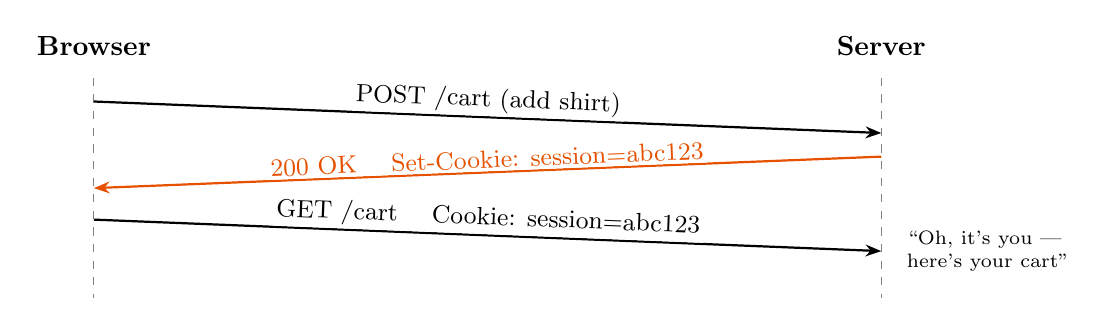
\begin{tikzpicture}
  \node[font=\bfseries] at (0,0.4) {Browser}; \node[font=\bfseries] at (10,0.4) {Server};
  \lifelines{0}{10}{0}{-2.8}
  \draw[msg] (0,-0.3) -- node[above,font=\small]{POST /cart (add shirt)} (10,-0.7);
  \draw[msg,cnorange] (10,-1.0) -- node[above,font=\small]{200 OK \quad Set-Cookie: session=abc123} (0,-1.4);
  \draw[msg] (0,-1.8) -- node[above,font=\small]{GET /cart \quad Cookie: session=abc123} (10,-2.2);
  \node[font=\scriptsize,align=left,anchor=west] at (10.2,-2.2) {``Oh, it's you ---\\here's your cart''};
\end{tikzpicture}
\end{center}

\section{HTTP generations: from HTTP/1.0 to HTTP/3}

\begin{analogy}[The online shopping delivery problem]
You order an outfit online: \textbf{shirt, pants, shoes and socks}. These are like the \textbf{HTML, CSS, JS and images} a web page requests from the server. How would you prefer them delivered? Your preference is the ``why'' behind every new HTTP version.
\end{analogy}

\subsection{HTTP/1.0 (1996) --- one item per trip}
\textbf{Analogy:} the truck can carry only one item per trip and must return to HQ before delivering the next. A massive waste of time.
\begin{itemize}
  \item One request at a time.
  \item Every file (HTML, image, CSS) = a \textbf{new TCP connection}.
  \item \textbf{No persistent} TCP connection $\Rightarrow$ slow, repetitive, inefficient (each new connection costs a handshake).
\end{itemize}

\subsection{HTTP/1.1 (1997) --- the one-truck convoy (Keep-Alive)}
\textbf{Analogy:} the truck arrives with all four items but unloads them one by one.
\begin{itemize}
  \item Introduced \textbf{Keep-Alive (persistent) connections}: many requests reuse one TCP connection.
  \item Introduced \textbf{caching} and the \textbf{Host header}.
  \item Better performance, but suffered from \textbf{head-of-line (HoL) blocking}.
\end{itemize}

\textbf{HTTP/1.1 pipelining (optional):}
\begin{itemize}
  \item Client can send multiple requests without waiting for each response.
  \item But responses must come back \textbf{in the same order} as requests (\textbf{FIFO} --- First In, First Out).
  \item Only \textbf{safe} methods can be pipelined (GET, HEAD, OPTIONS). Not POST/PUT, which have side effects.
\end{itemize}

\begin{keyidea}[Head-of-Line (HoL) blocking]
On one connection, responses must leave \textbf{in order}. If the first response (a slow image) is not ready, everything behind it (CSS, JS, icon) is \textbf{blocked}, even though they are ready. Like a queue at a shop where the first customer is still searching for their wallet.
\end{keyidea}

\begin{center}
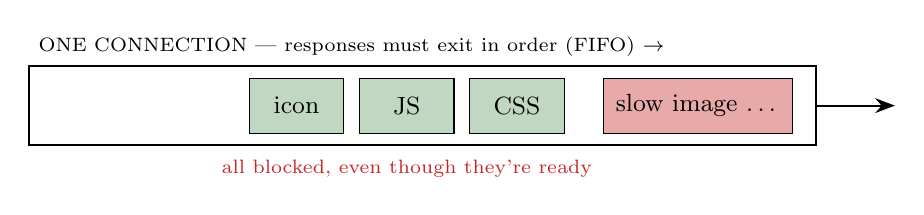
\begin{tikzpicture}
  \draw[thick] (0,0) rectangle (10,1);
  \node[font=\scriptsize,anchor=west] at (0,1.25) {ONE CONNECTION --- responses must exit in order (FIFO) $\rightarrow$};
  \node[draw,fill=cnred!40,minimum width=24mm,minimum height=7mm,font=\small] at (8.5,0.5) {slow image \ldots};
  \node[draw,fill=cngreen!30,minimum width=12mm,minimum height=7mm,font=\small] at (6.2,0.5) {CSS};
  \node[draw,fill=cngreen!30,minimum width=12mm,minimum height=7mm,font=\small] at (4.8,0.5) {JS};
  \node[draw,fill=cngreen!30,minimum width=12mm,minimum height=7mm,font=\small] at (3.4,0.5) {icon};
  \node[font=\scriptsize,cnred] at (4.8,-0.3) {all blocked, even though they're ready};
  \draw[arr] (10,0.5) -- (11,0.5);
\end{tikzpicture}
\end{center}
Browsers ``faked'' parallelism by opening about \textbf{6 separate TCP connections} per site --- costly: 6$\times$ setup, 6$\times$ overhead.

\subsection{HTTP/2 (2015) --- serve the whole tray}
\textbf{Analogy:} instead of serving your meal dish by dish, the waiter brings the entire tray and you choose what to eat.

HTTP/2 is the second major version, aimed at better performance by fixing HTTP/1.1's limits:
\begin{itemize}
  \item Uses a \textbf{single TCP connection}.
  \item \textbf{Binary protocol:} messages are encoded in a binary format (the \textbf{framing layer}), unlike text-based HTTP/1.x.
  \item \textbf{Multiplexing:} many requests and responses travel \textbf{simultaneously} over one connection as interleaved \textbf{streams}.
  \item \textbf{Server push:} the server can send resources \textbf{before the client asks} (e.g.\ send the CSS along with the HTML).
\end{itemize}

\begin{center}
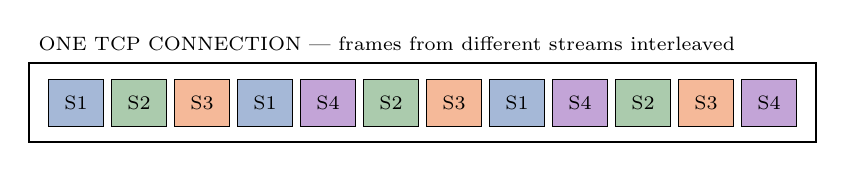
\begin{tikzpicture}
  \draw[thick] (0,0) rectangle (10,1);
  \node[font=\scriptsize,anchor=west] at (0,1.25) {ONE TCP CONNECTION --- frames from different streams interleaved};
  \foreach \x/\c/\t in {0.6/cnblue/1,1.4/cngreen/2,2.2/cnorange/3,3.0/cnblue/1,3.8/cnpurple/4,4.6/cngreen/2,5.4/cnorange/3,6.2/cnblue/1,7.0/cnpurple/4,7.8/cngreen/2,8.6/cnorange/3,9.4/cnpurple/4}
    \node[draw,fill=\c!40,minimum width=7mm,minimum height=6mm,font=\scriptsize] at (\x,0.5) {S\t};
\end{tikzpicture}
\end{center}

\textbf{But} HoL blocking still exists at the \textbf{TCP level}: TCP delivers bytes strictly in order, so if \textbf{one TCP segment is lost}, \textbf{all streams wait} until it's retransmitted.

\subsection{HTTP/3 with QUIC (June 2022)}
\textbf{Analogy:} you order 3 items in a restaurant and each item has its \textbf{own kitchen window and dedicated staff}. A delay in one dish doesn't hold up the others.
\begin{itemize}
  \item Latest version of HTTP.
  \item Built on \textbf{QUIC}, a \textbf{UDP-based} transport protocol developed by \textbf{Google}, instead of TCP.
  \item \textbf{Multiplexed streams without blocking} --- streams are truly independent.
  \item Designed to \textbf{solve head-of-line blocking}. TLS (encryption) is built into QUIC.
\end{itemize}

\begin{center}
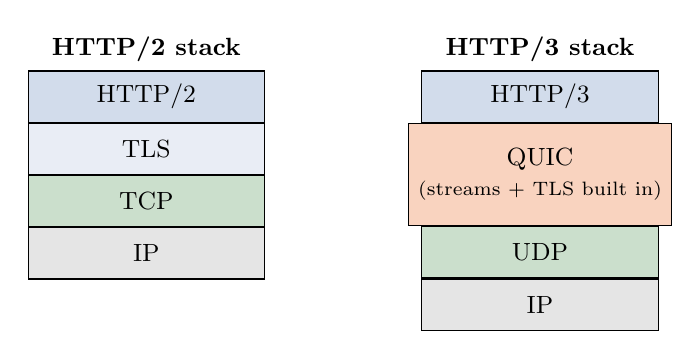
\begin{tikzpicture}[b/.style={draw,minimum width=30mm,minimum height=6.5mm,font=\small}]
  \node[font=\small\bfseries] at (0,0.6) {HTTP/2 stack};
  \node[b,fill=cnblue!20] (a1) at (0,0) {HTTP/2};
  \node[b,fill=cnblue!10,below=0mm of a1] (a2) {TLS};
  \node[b,fill=cngreen!25,below=0mm of a2] (a3) {TCP};
  \node[b,fill=gray!20,below=0mm of a3] (a4) {IP};
  \node[font=\small\bfseries] at (5,0.6) {HTTP/3 stack};
  \node[b,fill=cnblue!20] (b1) at (5,0) {HTTP/3};
  \node[b,fill=cnorange!25,below=0mm of b1,minimum height=13mm,align=center] (b2) {QUIC\\\scriptsize(streams + TLS built in)};
  \node[b,fill=cngreen!25,below=0mm of b2] (b3) {UDP};
  \node[b,fill=gray!20,below=0mm of b3] (b4) {IP};
\end{tikzpicture}
\end{center}

\subsection{Transition summary}
\begin{center}
\begin{tabularx}{\textwidth}{X X X}
\toprule
\textbf{HTTP/1.1} & \textbf{HTTP/2} & \textbf{HTTP/3} \\
\midrule
6 separate TCP connections to fake parallelism & Many streams multiplexed on one TCP connection & QUIC over UDP --- truly independent streams \\
Costly: 6$\times$ setup, 6$\times$ overhead & App-level HoL fixed; \textbf{TCP-level HoL remains}: 1 lost segment $\Rightarrow$ all streams stall & Loss is isolated to its own stream; only that stream waits \\
\bottomrule
\end{tabularx}
\end{center}

\begin{center}
\begin{tabular}{llll}
\toprule
Version & Year & Big idea & Remaining problem \\
\midrule
HTTP/1.0 & 1996 & one request per connection & very slow \\
HTTP/1.1 & 1997 & keep-alive, pipelining, Host header & HoL blocking (app level) \\
HTTP/2 & 2015 & binary, multiplexing, server push & HoL at TCP level \\
HTTP/3 & 2022 & QUIC over UDP & --- (solves HoL) \\
\bottomrule
\end{tabular}
\end{center}

\section{APIs and REST}
We understand client--server, where a browser asks a server for a page. But what happens when an \textbf{application needs to talk to another application}? It uses an \textbf{API}.

\subsection{REST APIs}
\textbf{REST} (REpresentational State Transfer) is the most popular style of web API: a Q4 2024 analysis estimated \textbf{83\% of all public APIs use REST}.

\textbf{REST basics:} the client sends HTTP requests (GET, POST, PUT, PATCH, DELETE) to a URL (an \emph{endpoint} that names a \emph{resource}); the REST API talks to the database and sends back a response, typically in \textbf{JSON} (or XML).

\begin{center}
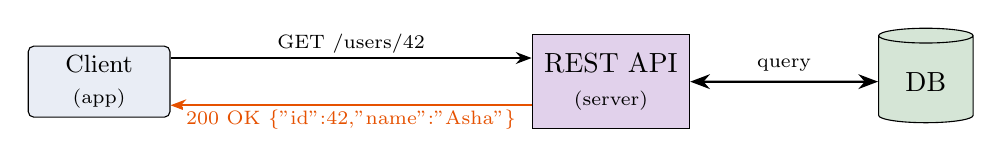
\begin{tikzpicture}
  \node[host,minimum width=18mm] (c) at (0,0) {Client\\\scriptsize(app)};
  \node[draw,fill=cnpurple!20,minimum width=20mm,minimum height=12mm,align=center] (api) at (6.5,0) {REST API\\\scriptsize(server)};
  \node[draw,cylinder,shape border rotate=90,aspect=0.25,fill=cngreen!20,minimum height=12mm,minimum width=12mm] (db) at (10.5,0) {DB};
  \draw[msg] ([yshift=3mm]c.east) -- node[above,font=\scriptsize]{GET /users/42} ([yshift=3mm]api.west);
  \draw[msg,cnorange] ([yshift=-3mm]api.west) -- node[below,font=\scriptsize]{200 OK \{"id":42,"name":"Asha"\}} ([yshift=-3mm]c.east);
  \draw[darr] (api) -- node[above,font=\scriptsize]{query} (db);
\end{tikzpicture}
\end{center}

\textbf{REST principles} (the rules that make an API ``RESTful''):
\begin{itemize}
  \item \textbf{Client--server:} client and server are separate; they only share the API contract.
  \item \textbf{Stateless:} every request carries all information needed --- the server keeps no session memory (just like HTTP).
  \item \textbf{Resources identified by URLs:} e.g.\ \texttt{/users}, \texttt{/users/42}.
  \item \textbf{Uniform interface:} use standard HTTP methods for actions --- GET (read), POST (create), PUT/PATCH (update), DELETE (remove).
  \item \textbf{Representations:} data is sent as JSON/XML.
  \item \textbf{Cacheable:} responses say whether they can be cached.
\end{itemize}

\begin{center}
\begin{tabular}{>{\ttfamily}l >{\ttfamily}l l}
\toprule
\textrm{Method} & \textrm{Endpoint} & Meaning \\
\midrule
GET & /users & list all users \\
GET & /users/42 & read user 42 \\
POST & /users & create a new user \\
PUT & /users/42 & update user 42 \\
DELETE & /users/42 & delete user 42 \\
\bottomrule
\end{tabular}
\end{center}

\subsection{Why use OpenAPI?}
\textbf{OpenAPI} (Swagger) is a standard way to \textbf{describe} a REST API in a file --- its endpoints, methods, inputs and outputs. It acts as a \textbf{contract}: the \textbf{API producer} defines and publishes it; \textbf{API consumers} (front-end developers, third-party developers, AI agents, testing tools) read it to know exactly how to call the API. Demo: \url{https://petstore3.swagger.io}.

\begin{recap}
\begin{itemize}
  \item Client/Server (central server) vs P2P (everyone is client and server).
  \item Application layer (L7) = interface between apps and network. Protocols: HTTP(S), FTP, SMTP, Telnet, DNS.
  \item HTTP is stateless request--response over TCP. Message = start line + headers + empty line + optional body.
  \item Request line = Method + URL + Version. Status line = Version + Code + Message.
  \item Codes: 200 OK, 301 permanent, 302 temporary, 403 forbidden, 404 not found, 500 server error.
  \item State is added with cookies / session tokens.
  \item 1.0: new connection per file. 1.1: keep-alive, pipelining (FIFO, safe methods), HoL blocking. 2: binary, multiplexing, server push, one TCP conn (TCP HoL remains). 3: QUIC over UDP, no HoL.
  \item REST: stateless, resources as URLs, HTTP methods, JSON. 83\% of public APIs. OpenAPI = API contract.
\end{itemize}
\end{recap}

\chapter{Lecture 6 --- HTTPS and the TLS Handshake: Securing the Web}

\begin{keyidea}[The one idea from this lecture]
Plain HTTP sends everything as readable text, so anyone in the middle can read or change it. \textbf{HTTPS = HTTP + TLS}. TLS uses \textbf{cryptography} to give three things: \textbf{confidentiality} (no eavesdropping), \textbf{integrity} (no tampering) and \textbf{authentication} (verified identity). It uses \textbf{asymmetric} encryption to safely agree on a key, then fast \textbf{symmetric} encryption for the actual data. \textbf{Certificates} signed by trusted \textbf{CAs} prove the server is who it claims to be.
\end{keyidea}

\textbf{Roadmap:} HTTP over TLS (HTTPS) $\cdot$ Cryptography and its goals $\cdot$ Encryption types $\cdot$ TLS handshake flow $\cdot$ CAs and chain of trust $\cdot$ HTTPS in AWS.

\section{Recap and the padlock question}
In the HTTP/2 vs HTTP/3 stacks from Lecture 5, there is a ``security'' layer: \textbf{TLS} sits between HTTP and TCP (in HTTP/3 it is built into QUIC). Without it, data travels as \textbf{plain text}.

\textbf{What does the padlock in the browser mean?}
\begin{center}
\begin{tabular}{lc}
\toprule
Claim & True? \\
\midrule
The website is \emph{safe} (not a scam) & \textcolor{cnred}{\ding{55}\ No} \\
The connection is \emph{encrypted} & \textcolor{cngreen}{\checkmark\ Yes} \\
The server's \emph{identity is verified} (it really owns that domain) & \textcolor{cngreen}{\checkmark\ Yes} \\
\bottomrule
\end{tabular}
\end{center}
A phishing site can have a padlock too! The padlock only says ``nobody can read this conversation, and you're talking to the real owner of \emph{this} domain''.

\section{HTTP is plain text by design}
\begin{itemize}
  \item HTTP has \textbf{no built-in security}; it is vulnerable unless HTTPS is used.
  \item Anyone who can \textbf{capture the traffic} (on public WiFi, at the ISP, \ldots) can read the full conversation between client and server --- passwords included.
\end{itemize}

\begin{center}
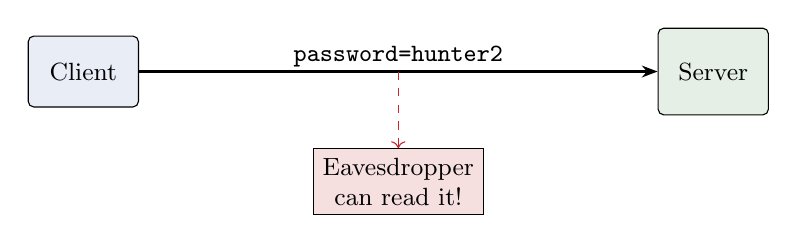
\begin{tikzpicture}
  \node[host] (c) at (0,0) {Client};
  \node[srv] (s) at (8,0) {Server};
  \draw[msg] (c) -- node[above,font=\ttfamily\small]{password=hunter2} (s);
  \node[draw,fill=cnred!15,font=\small,align=center] (e) at (4,-1.4) {Eavesdropper\\can read it!};
  \draw[dashed,cnred,->] (4,0) -- (e);
\end{tikzpicture}
\end{center}

\section{HTTPS = HTTP + TLS}
\begin{itemize}
  \item \textbf{HTTPS} is the secure version of HTTP for safe communication over networks (port 443).
  \item Historically it used \textbf{SSL} (Secure Sockets Layer).
  \item Today it uses \textbf{TLS} (Transport Layer Security) to \textbf{encrypt data between client and server}.
\end{itemize}
\textbf{What does TLS actually provide?} \emph{Security, using cryptography.}

\section{Cryptography}
\textbf{Cryptography} is the practice of securing information by converting readable text (\textbf{plaintext}) into unreadable code (\textbf{ciphertext}) and back again.

\begin{center}
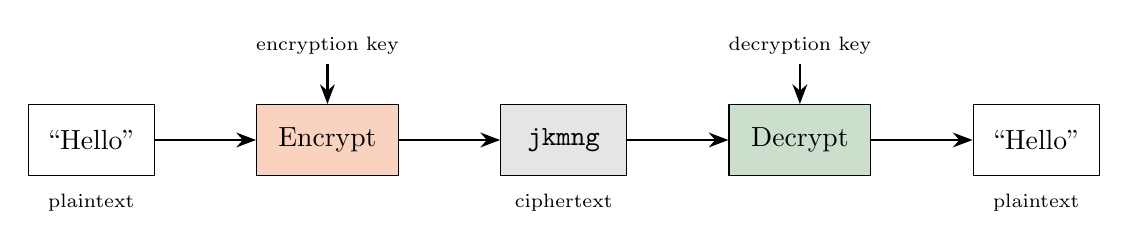
\begin{tikzpicture}
  \node[draw,fill=white,minimum width=16mm,minimum height=9mm] (p1) at (0,0) {``Hello''};
  \node[draw,fill=cnorange!25,minimum width=18mm,minimum height=9mm] (e) at (3,0) {Encrypt};
  \node[draw,fill=gray!20,minimum width=16mm,minimum height=9mm,font=\ttfamily] (c) at (6,0) {jkmng};
  \node[draw,fill=cngreen!25,minimum width=18mm,minimum height=9mm] (d) at (9,0) {Decrypt};
  \node[draw,fill=white,minimum width=16mm,minimum height=9mm] (p2) at (12,0) {``Hello''};
  \draw[arr] (p1) -- (e); \draw[arr] (e) -- (c); \draw[arr] (c) -- (d); \draw[arr] (d) -- (p2);
  \node[font=\scriptsize] (k1) at (3,1.2) {encryption key}; \draw[arr] (k1) -- (e);
  \node[font=\scriptsize] (k2) at (9,1.2) {decryption key}; \draw[arr] (k2) -- (d);
  \node[font=\scriptsize,below=1mm of p1] {plaintext}; \node[font=\scriptsize,below=1mm of c] {ciphertext}; \node[font=\scriptsize,below=1mm of p2] {plaintext};
\end{tikzpicture}
\end{center}

\subsection{Core goals of cryptography}
\begin{center}
\begin{tabularx}{\textwidth}{>{\bfseries}l X l}
\toprule
Goal & Meaning & Slogan \\
\midrule
Confidentiality (privacy) & Information is accessible \textbf{only to authorised parties}. & ``No eavesdropping'' \\
Integrity & Data stays accurate and \textbf{hasn't been altered} in transit or storage. & ``No tampering'' \\
Authentication & Verifies the \textbf{identities} of sender and receiver. & ``Verified identity'' \\
\bottomrule
\end{tabularx}
\end{center}

\section{How do we achieve these goals? Encryption}

\subsection{Symmetric encryption}
\textbf{One shared secret key} is used both to encrypt and to decrypt.
\begin{center}
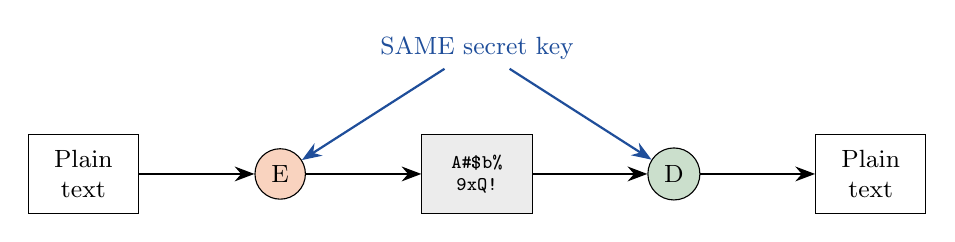
\begin{tikzpicture}
  \node[draw,minimum width=14mm,minimum height=10mm,font=\small,align=center] (p) at (0,0) {Plain\\text};
  \node[draw,circle,fill=cnorange!25,font=\small] (e) at (2.5,0) {E};
  \node[draw,minimum width=14mm,minimum height=10mm,font=\ttfamily\scriptsize,fill=gray!15,align=center] (c) at (5,0) {A\#\$b\%\\9xQ!};
  \node[draw,circle,fill=cngreen!25,font=\small] (d) at (7.5,0) {D};
  \node[draw,minimum width=14mm,minimum height=10mm,font=\small,align=center] (p2) at (10,0) {Plain\\text};
  \draw[arr] (p) -- (e); \draw[arr] (e) -- (c); \draw[arr] (c) -- (d); \draw[arr] (d) -- (p2);
  \node[font=\small,cnblue] (k) at (5,1.6) {SAME secret key};
  \draw[arr,cnblue] (k) -- (e); \draw[arr,cnblue] (k) -- (d);
\end{tikzpicture}
\end{center}
\begin{itemize}
  \item \textbf{Fast} --- great for encrypting lots of data.
  \item \textbf{The issue:} \emph{how do we share the key securely?} If you send the key over the network, an eavesdropper can grab it. \textbf{Strangers (your browser and a website you've never visited) cannot securely share a key in advance.}
\end{itemize}

\subsection{Asymmetric (public-key) encryption}
Each party has a \textbf{key pair}: a \textbf{public key} (shared with everyone) and a \textbf{private key} (kept secret). Data encrypted with the public key can \textbf{only} be decrypted with the matching private key.
\begin{center}
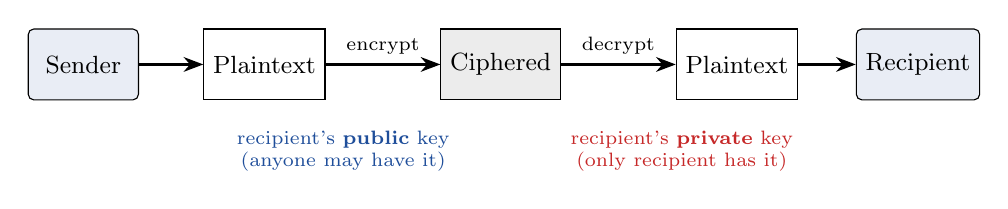
\begin{tikzpicture}
  \node[host] (s) at (0,0) {Sender};
  \node[draw,minimum width=14mm,minimum height=9mm,font=\small] (p) at (2.3,0) {Plaintext};
  \node[draw,fill=gray!15,minimum width=14mm,minimum height=9mm,font=\small] (c) at (5.3,0) {Ciphered};
  \node[draw,minimum width=14mm,minimum height=9mm,font=\small] (p2) at (8.3,0) {Plaintext};
  \node[host] (r) at (10.6,0) {Recipient};
  \draw[arr] (s) -- (p); \draw[arr] (p) -- node[above,font=\scriptsize]{encrypt} (c); \draw[arr] (c) -- node[above,font=\scriptsize]{decrypt} (p2); \draw[arr] (p2) -- (r);
  \node[font=\scriptsize,cnblue,align=center] at (3.3,-1.1) {recipient's \textbf{public} key\\(anyone may have it)};
  \node[font=\scriptsize,cnred,align=center] at (7.6,-1.1) {recipient's \textbf{private} key\\(only recipient has it)};
\end{tikzpicture}
\end{center}
\begin{itemize}
  \item Solves the key-sharing problem: you can publish your public key freely.
  \item But it is \textbf{slow} --- too slow to encrypt a whole video stream.
\end{itemize}

\begin{keyidea}[Key insight of TLS: use BOTH]
\textbf{Asymmetric} $\to$ to share a secret safely (only at the start). \\
\textbf{Symmetric} $\to$ for fast communication (all the actual data). \\
Why not only symmetric? Because strangers cannot securely share a key. Why not only asymmetric? Because it is slow.
\end{keyidea}

\begin{center}
\begin{tabular}{lll}
\toprule
 & Symmetric & Asymmetric \\
\midrule
Keys & 1 shared secret key & Public + private key pair \\
Speed & Fast & Slow \\
Problem & How to share the key? & Too slow for bulk data \\
Used in TLS for & Encrypting the data (session key) & Safely exchanging the secret \\
\bottomrule
\end{tabular}
\end{center}

\section{How do I trust this server? Certificates}
Look at these two domains: \texttt{micr\underline{o}s\underline{o}ft.com} vs \texttt{microsoft.com}. In the first one the underlined letters are actually Cyrillic ``o'' characters --- it looks identical but is a \textbf{different site}. Encryption alone is useless if you're encrypting your password \emph{to an attacker}. We need proof of identity: a \textbf{certificate}.

\subsection{What is a certificate?}
A \textbf{digital certificate} is like an ID card for a website. It contains:
\begin{itemize}
  \item the \textbf{domain name} it is issued to (Common Name, e.g.\ \texttt{*.canva.com}),
  \item the server's \textbf{public key},
  \item the \textbf{issuer} --- the \textbf{Certificate Authority (CA)} that vouches for it (e.g.\ Amazon RSA 2048 M04),
  \item \textbf{validity dates} (e.g.\ expires on some date) and a serial number,
  \item the CA's \textbf{digital signature}, proving the CA really issued it.
\end{itemize}

\subsection{CAs and the chain of trust}
Your browser/OS ships with a list of trusted \textbf{root CAs}. A root CA signs an \textbf{intermediate CA}'s certificate, which signs the website's certificate. The browser checks each signature up the chain until it reaches a root it already trusts.
\begin{center}
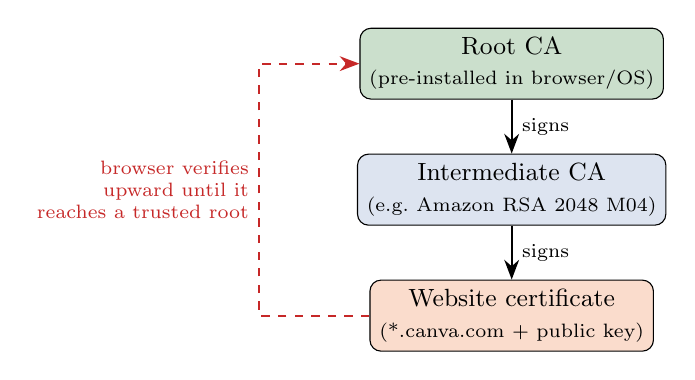
\begin{tikzpicture}[c/.style={draw,rounded corners,minimum width=36mm,minimum height=9mm,align=center,font=\small}]
  \node[c,fill=cngreen!25] (r) at (0,0) {Root CA\\\scriptsize(pre-installed in browser/OS)};
  \node[c,fill=cnblue!15] (i) at (0,-1.6) {Intermediate CA\\\scriptsize(e.g.\ Amazon RSA 2048 M04)};
  \node[c,fill=cnorange!20] (l) at (0,-3.2) {Website certificate\\\scriptsize(*.canva.com + public key)};
  \draw[arr] (r) -- node[right,font=\scriptsize]{signs} (i);
  \draw[arr] (i) -- node[right,font=\scriptsize]{signs} (l);
  \draw[arr,dashed,cnred] (l.west) -- ++(-1.4,0) |- node[pos=0.25,left,font=\scriptsize,align=right]{browser verifies\\upward until it\\reaches a trusted root} (r.west);
\end{tikzpicture}
\end{center}

\subsection{How HTTPS works (big picture)}
\begin{center}
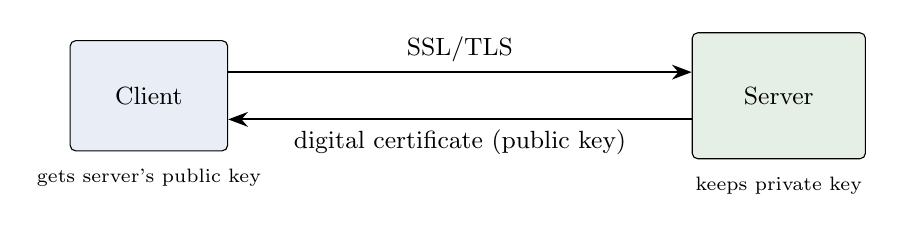
\begin{tikzpicture}
  \node[host,minimum width=20mm,minimum height=14mm] (c) at (0,0) {Client};
  \node[srv,minimum width=22mm,minimum height=16mm] (s) at (8,0) {Server};
  \draw[arr] ([yshift=3mm]c.east) -- node[above,font=\small]{SSL/TLS} ([yshift=3mm]s.west);
  \draw[arr] ([yshift=-3mm]s.west) -- node[below,font=\small]{digital certificate (public key)} ([yshift=-3mm]c.east);
  \node[below=1mm of c,font=\scriptsize] {gets server's public key};
  \node[below=1mm of s,font=\scriptsize] {keeps private key};
\end{tikzpicture}
\end{center}
Three phases: \textcircled{1} \textbf{server certificate check}, \textcircled{2} \textbf{key exchange}, \textcircled{3} \textbf{encrypted tunnel} for data.

\section{The TLS handshake}
TLS runs \textbf{after} the TCP 3-way handshake (Lecture 9) and \textbf{before} any HTTP data is sent.

\begin{center}
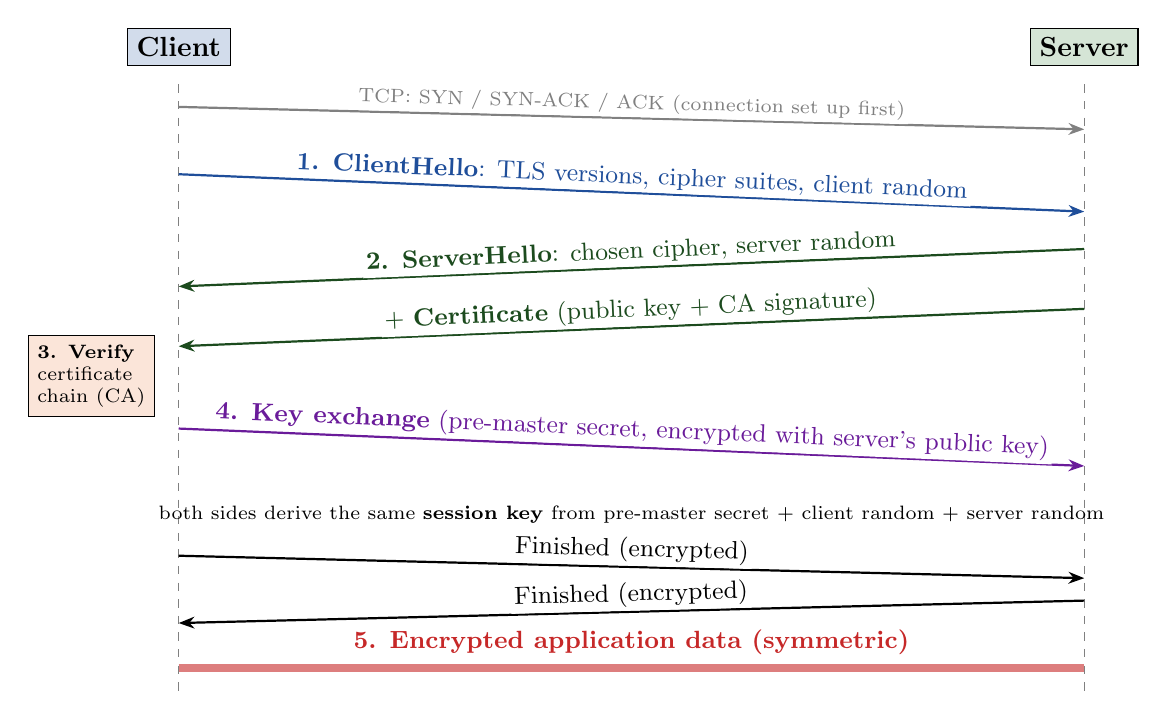
\begin{tikzpicture}[yscale=0.95]
  \node[draw,fill=cnblue!20,font=\bfseries] at (0,0.5) {Client};
  \node[draw,fill=cngreen!20,font=\bfseries] at (11.5,0.5) {Server};
  \lifelines{0}{11.5}{0}{-8.2}
  \draw[msg,gray] (0,-0.3) -- node[above,font=\scriptsize]{TCP: SYN / SYN-ACK / ACK (connection set up first)} (11.5,-0.6);
  \draw[msg,cnblue] (0,-1.2) -- node[above,font=\small]{\textbf{1. ClientHello}: TLS versions, cipher suites, client random} (11.5,-1.7);
  \draw[msg,cngreen!60!black] (11.5,-2.2) -- node[above,font=\small]{\textbf{2. ServerHello}: chosen cipher, server random} (0,-2.7);
  \draw[msg,cngreen!60!black] (11.5,-3.0) -- node[above,font=\small]{+ \textbf{Certificate} (public key + CA signature)} (0,-3.5);
  \node[draw,fill=cnorange!15,font=\scriptsize,align=left,anchor=east] at (-0.3,-3.9) {\textbf{3. Verify}\\certificate\\chain (CA)};
  \draw[msg,cnpurple] (0,-4.6) -- node[above,font=\small]{\textbf{4. Key exchange} (pre-master secret, encrypted with server's public key)} (11.5,-5.1);
  \node[font=\scriptsize,align=center] at (5.75,-5.75) {both sides derive the same \textbf{session key} from pre-master secret + client random + server random};
  \draw[msg] (0,-6.3) -- node[above,font=\small]{Finished (encrypted)} (11.5,-6.6);
  \draw[msg] (11.5,-6.9) -- node[above,font=\small]{Finished (encrypted)} (0,-7.2);
  \draw[line width=3pt,cnred!60] (0,-7.8) -- node[above,font=\small\bfseries,text=cnred]{5. Encrypted application data (symmetric)} (11.5,-7.8);
\end{tikzpicture}
\end{center}

\subsection*{Step 1 --- ClientHello}
The client offers the \textbf{TLS versions} and \textbf{cipher suites} (bundles of algorithms) it supports, plus a \textbf{random nonce} (a 32-byte number used once).
\begin{quote}\emph{``I can speak TLS 1.3 or TLS 1.2. I can use XYZ algorithm for PQR purposes. Here is a number-used-once, a 32-byte string.''}\end{quote}

\subsection*{Step 2 --- ServerHello + Certificate}
The server replies with the \textbf{cipher it picked} and its \textbf{certificate} (public key + CA signature).
\begin{quote}\emph{``Out of your options, we will use this bundle of algorithms to encrypt our session, and this is my identity, issued by the following authority.''}\end{quote}

\subsection*{Step 3 --- Authentication}
The client \textbf{validates the certificate chain}: is it signed by a trusted CA, does the hostname match, is it unexpired / not revoked? If valid, the client can trust the server; if not, the browser shows ``\textbf{Your connection is not private / website is not secure}''. \textbf{This step stops man-in-the-middle attacks}, because an attacker cannot get a CA-signed certificate for someone else's domain.

\subsection*{Step 4 --- Key exchange}
Client and server \textbf{derive a shared session key}. (Classic way: the client makes a \emph{pre-master secret}, encrypts it with the server's public key; only the server's private key can decrypt it. Both sides then mix it with the two random numbers to get the same symmetric key. TLS 1.3 uses Diffie--Hellman, with the same result: a shared key no eavesdropper knows.)

\subsection*{Step 5 --- Data sharing on a secure channel}
Communication starts: all \textbf{application data is encrypted} with the symmetric session key --- an \textbf{encrypted tunnel}.

\begin{examtip}
Know the order: \textbf{ClientHello $\to$ ServerHello + Certificate $\to$ Certificate validation $\to$ Key exchange $\to$ Encrypted data.} And know \emph{why} each exists: Hello = agree on algorithms; Certificate = authentication; Key exchange (asymmetric) = safely agree a secret; Data (symmetric) = speed.
\end{examtip}

\section{Real-world deployment: HTTPS in AWS}
\textbf{Lab objective:} add a certificate using \textbf{AWS Certificate Manager (ACM)}. ACM issues (free) TLS certificates for your domain and attaches them to AWS services such as load balancers or CloudFront, so your site is served over HTTPS. ACM also handles renewal.

\begin{recap}
\begin{itemize}
  \item Padlock = encrypted + identity verified; NOT ``the site is safe''.
  \item HTTP = plain text. HTTPS = HTTP + TLS (formerly SSL), port 443.
  \item Cryptography: plaintext $\leftrightarrow$ ciphertext. Goals: Confidentiality, Integrity, Authentication.
  \item Symmetric: 1 key, fast, key-sharing problem. Asymmetric: public/private pair, solves sharing, slow. TLS uses both.
  \item Certificate = domain + public key + issuer CA + validity + CA signature. Chain of trust: root $\to$ intermediate $\to$ site.
  \item Handshake: ClientHello $\to$ ServerHello+Cert $\to$ verify $\to$ key exchange $\to$ encrypted data.
  \item AWS ACM provides certificates.
\end{itemize}
\end{recap}

\chapter{Lecture 7 --- Email Protocols (SMTP, POP3, IMAP), CDNs and Caching}

\begin{keyidea}[The one idea from this lecture]
Email uses two kinds of protocol: \textbf{SMTP} to \textbf{push} (send) mail between servers, and \textbf{POP3} or \textbf{IMAP} to \textbf{pull} (read) mail from your mailbox. Then: if the same content is requested again and again, don't fetch it from far away every time --- keep a copy close by. That is \textbf{caching}, and a world-wide network of caches is a \textbf{CDN}.
\end{keyidea}

\section{Recap: application layer protocols}
HTTP/HTTPS for the web (Lectures 5--6). Today: email protocols and fast content delivery.

\section{How email travels}

\begin{center}
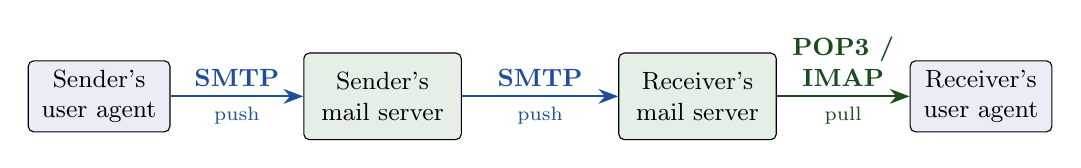
\begin{tikzpicture}
  \node[host,minimum width=18mm] (sua) at (0,0) {Sender's\\user agent};
  \node[srv,minimum width=20mm] (sms) at (3.6,0) {Sender's\\mail server};
  \node[srv,minimum width=20mm] (rms) at (7.6,0) {Receiver's\\mail server};
  \node[host,minimum width=18mm] (rua) at (11.2,0) {Receiver's\\user agent};
  \draw[arr,cnblue] (sua) -- node[above,font=\small\bfseries]{SMTP} node[below,font=\scriptsize]{push} (sms);
  \draw[arr,cnblue] (sms) -- node[above,font=\small\bfseries]{SMTP} node[below,font=\scriptsize]{push} (rms);
  \draw[arr,cngreen!60!black] (rms) -- node[above,font=\small\bfseries,align=center]{POP3 /\\IMAP} node[below,font=\scriptsize]{pull} (rua);
\end{tikzpicture}
\end{center}

\subsection{How SMTP works}
\begin{enumerate}
  \item The email client (Gmail app, Outlook) connects to the \textbf{SMTP server}.
  \item SMTP \textbf{pushes} the message from the sender to the \textbf{receiver's mail server}.
  \item The receiver then uses \textbf{POP3 or IMAP} to retrieve the email.
\end{enumerate}

\section{SMTP --- Simple Mail Transfer Protocol (email \emph{server} protocol)}
\begin{itemize}
  \item \textbf{Sends} email from the sender's server to the recipient's server.
  \item \textbf{Push-based} protocol.
  \item Uses \textbf{TCP}, ports \textbf{25 / 587 / 465} (25 = server-to-server, 587 = submission with STARTTLS, 465 = SMTP over TLS).
  \item \textbf{In the real world:} services such as \textbf{SendGrid, Mailchimp, Mailgun} offer \textbf{SMTP relays} that apps integrate with to send mail. \textbf{MailHog} is a tool for testing SMTP locally (it catches emails instead of delivering them).
\end{itemize}

\section{Email client protocols (reading mail)}

\subsection{IMAP --- Internet Message Access Protocol}
\begin{itemize}
  \item Manages email \textbf{directly on the server} --- messages stay on the server.
  \item Suitable for \textbf{multi-device access} (phone, laptop, web all see the same inbox).
  \item Supports \textbf{folders} and \textbf{partial downloads}.
  \item Ports: \textbf{143}, secure IMAPS: \textbf{993}.
  \item Connection type: \textbf{two-way sync} (client $\leftrightarrow$ server).
\end{itemize}
\textbf{How IMAP works:}
\begin{enumerate}
  \item The email client connects to the server using IMAP.
  \item You view and manage emails \textbf{without downloading them completely}.
  \item Changes (read/unread, folders, deletions) are \textbf{reflected on the server} and \textbf{synced across all devices}.
  \item You see folders (Inbox, Sent, Drafts, \ldots) as organised on the server.
\end{enumerate}

\subsection{POP3 --- Post Office Protocol version 3}
\begin{itemize}
  \item \textbf{Downloads} email to the local client and \textbf{deletes it from the server}.
  \item Best for \textbf{offline access}, but \textbf{poor sync} across devices.
  \item Ports: \textbf{110}, secure POP3S: \textbf{995}.
  \item Connection type: \textbf{one-way} (server $\to$ client).
\end{itemize}
\textbf{How POP3 works:}
\begin{enumerate}
  \item The client connects to the mail server using POP3.
  \item It downloads the emails.
  \item It deletes them from the server.
  \item Emails now exist \textbf{only on your local device}.
\end{enumerate}

\begin{center}
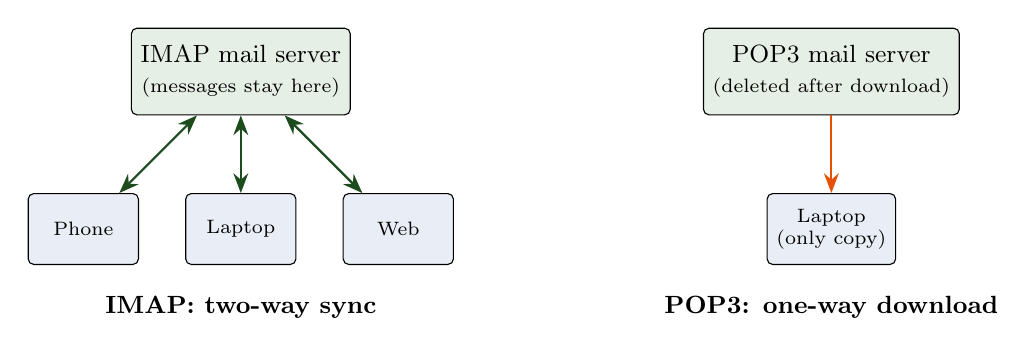
\begin{tikzpicture}
  \begin{scope}
    \node[srv,minimum width=22mm] (s) at (0,0) {IMAP mail server\\\scriptsize(messages stay here)};
    \node[host,font=\scriptsize] (p) at (-2,-2) {Phone};
    \node[host,font=\scriptsize] (l) at (0,-2) {Laptop};
    \node[host,font=\scriptsize] (w) at (2,-2) {Web};
    \foreach \d in {p,l,w} \draw[darr,cngreen!60!black] (s) -- (\d);
    \node[font=\small\bfseries] at (0,-3) {IMAP: two-way sync};
  \end{scope}
  \begin{scope}[xshift=7.5cm]
    \node[srv,minimum width=22mm] (s2) at (0,0) {POP3 mail server\\\scriptsize(deleted after download)};
    \node[host,font=\scriptsize] (l2) at (0,-2) {Laptop\\(only copy)};
    \draw[arr,cnorange] (s2) -- (l2);
    \node[font=\small\bfseries] at (0,-3) {POP3: one-way download};
  \end{scope}
\end{tikzpicture}
\end{center}

\subsection{Comparison}
\begin{center}
\begin{tabularx}{\textwidth}{>{\bfseries}l X X X}
\toprule
 & SMTP & IMAP & POP3 \\
\midrule
Purpose & Send / transfer mail & Read \& manage mail on server & Download mail to device \\
Direction & Push & Two-way sync & One-way (server $\to$ client) \\
Where mail lives & --- & On the server & On your device (deleted from server) \\
Multi-device & --- & Excellent & Poor \\
Ports & 25 / 587 / 465 & 143 / 993 (IMAPS) & 110 / 995 (POP3S) \\
Transport & TCP & TCP & TCP \\
\bottomrule
\end{tabularx}
\end{center}

\begin{examtip}
SMTP = \textbf{S}ends (push). POP3 = \textbf{P}ulls and removes (like picking letters out of a Post-Office box). IMAP = keeps everything on the server and \textbf{syncs}. Learn the port numbers!
\end{examtip}

\section{Quick and efficient content delivery}

\subsection{The problem}
Imagine the \textbf{same content is requested repeatedly} (the same logo, the same viral video). Fetching it from a far-away origin server each time wastes time and bandwidth. \textbf{Solution: caching.}

\section{Caching}
\textbf{Caching} is storing copies of data in a \textbf{temporary, high-speed storage layer} so future requests for the same data can be served much faster than fetching from the original, slower source.

\begin{itemize}
  \item \textbf{Cache hit:} the data is in the cache $\Rightarrow$ served immediately.
  \item \textbf{Cache miss:} not in the cache $\Rightarrow$ fetch from the origin, then (usually) store a copy for next time.
\end{itemize}

\begin{center}
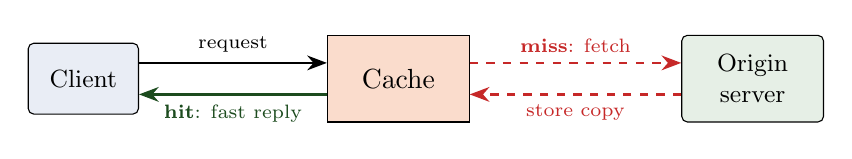
\begin{tikzpicture}
  \node[host] (c) at (0,0) {Client};
  \node[draw,fill=cnorange!20,minimum width=18mm,minimum height=11mm] (k) at (4,0) {Cache};
  \node[srv,minimum width=18mm] (o) at (8.5,0) {Origin\\server};
  \draw[arr] ([yshift=2mm]c.east) -- node[above,font=\scriptsize]{request} ([yshift=2mm]k.west);
  \draw[arr,cngreen!60!black] ([yshift=-2mm]k.west) -- node[below,font=\scriptsize]{\textbf{hit}: fast reply} ([yshift=-2mm]c.east);
  \draw[arr,cnred,dashed] ([yshift=2mm]k.east) -- node[above,font=\scriptsize]{\textbf{miss}: fetch} ([yshift=2mm]o.west);
  \draw[arr,cnred,dashed] ([yshift=-2mm]o.west) -- node[below,font=\scriptsize]{store copy} ([yshift=-2mm]k.east);
\end{tikzpicture}
\end{center}

\subsection{Caching behaviour}
How data is stored temporarily and retrieved to improve performance and reduce latency. Used widely in networking, browsers, web servers, CDNs and applications.

\subsection{The Cache-Control header}
The server tells clients/caches how to cache a response with an HTTP header:
\begin{lstlisting}
Cache-Control: public, max-age=3600
\end{lstlisting}
\begin{itemize}
  \item \texttt{public} --- any cache (browser, proxy, CDN) may store it.
  \item \texttt{max-age=3600} --- the copy is fresh for 3600 seconds (1 hour).
  \item (Other common values: \texttt{private} = only the user's browser; \texttt{no-cache} = must revalidate before use; \texttt{no-store} = never store.)
\end{itemize}

\subsection{How caching works (step by step)}
\begin{enumerate}
  \item A client requests a resource (e.g.\ an image, a CSS file).
  \item The server responds and may include \textbf{cache-control headers}.
  \item The client stores the resource in its \textbf{local cache}.
  \item On the next request, the client checks: \emph{is the cached copy still valid (not expired)?}
  \begin{itemize}
    \item \textbf{Valid} $\to$ use it from cache (\textbf{no network trip}).
    \item \textbf{Expired} $\to$ \textbf{revalidate} with the server or fetch again.
  \end{itemize}
\end{enumerate}

\subsection{Layers of caching}
\begin{center}
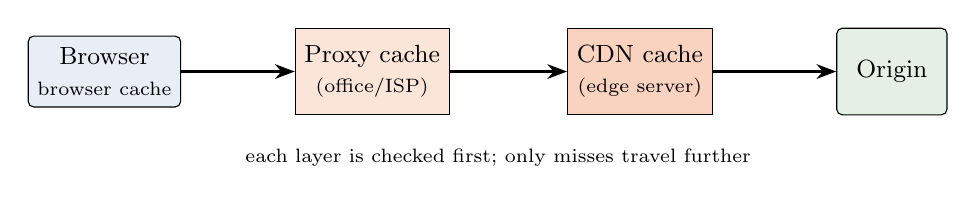
\begin{tikzpicture}
  \node[host] (u) at (0,0) {Browser\\\scriptsize browser cache};
  \node[draw,fill=cnorange!15,minimum height=11mm,align=center,font=\small] (p) at (3.4,0) {Proxy cache\\\scriptsize(office/ISP)};
  \node[draw,fill=cnorange!25,minimum height=11mm,align=center,font=\small] (cdn) at (6.8,0) {CDN cache\\\scriptsize(edge server)};
  \node[srv] (o) at (10,0) {Origin};
  \draw[arr] (u) -- (p); \draw[arr] (p) -- (cdn); \draw[arr] (cdn) -- (o);
  \node[font=\scriptsize] at (5,-1.1) {each layer is checked first; only misses travel further};
\end{tikzpicture}
\end{center}
\begin{enumerate}
  \item \textbf{Browser caching} --- on your own device.
  \item \textbf{Proxy cache} --- shared by many users of an organisation or ISP.
  \item \textbf{CDN cache} --- edge servers spread around the world.
\end{enumerate}

\section{Content Delivery Networks (CDNs)}

\begin{analogy}[A chain of grocery stores]
Instead of travelling to faraway farms, shoppers visit a \textbf{local store}. Local stores stock food from distant farms, saving time and effort. Similarly, CDNs \textbf{cache web content close to users}. Result: pages load in moments, just like shopping takes minutes, not days.
\end{analogy}

A \textbf{CDN} is a set of \textbf{geographically distributed servers} that deliver content from the \textbf{nearest edge server}, reducing latency and saving bandwidth.

\subsection{How a CDN works}
\begin{enumerate}
  \item A user requests content (e.g.\ a video or image) from a website.
  \item The \textbf{nearest edge server} serves the request instead of the origin server.
  \item If the content is not cached, the edge server \textbf{retrieves it from the origin and caches it}.
\end{enumerate}

\begin{center}
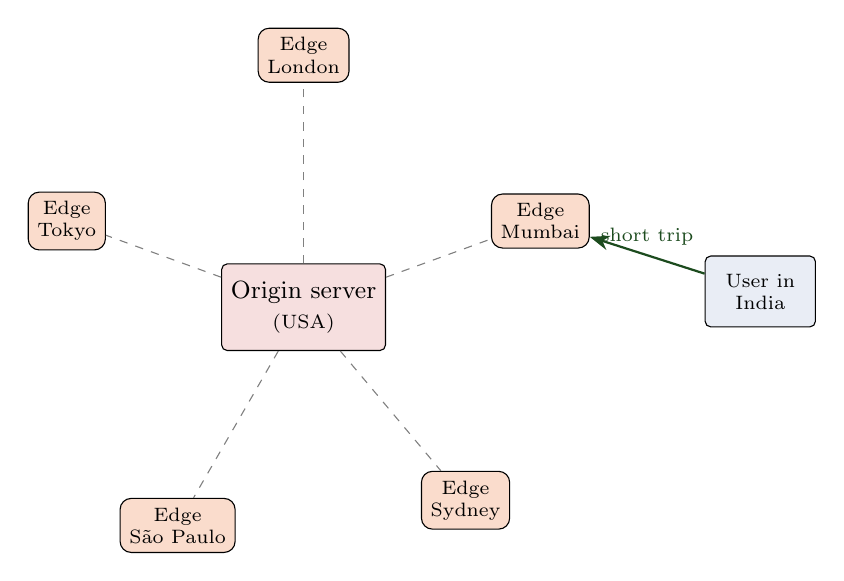
\begin{tikzpicture}
  \node[srv,minimum width=20mm,fill=cnred!15] (o) at (0,0) {Origin server\\\scriptsize(USA)};
  \foreach \a/\n/\l in {20/e1/Mumbai,90/e2/London,160/e3/Tokyo,240/e4/S\~ao Paulo,310/e5/Sydney} {
    \node[draw,fill=cnorange!20,rounded corners,font=\scriptsize,align=center] (\n) at (\a:3.2) {Edge\\\l};
    \draw[gray,dashed] (o) -- (\n);
  }
  \node[host,font=\scriptsize] (u) at (5.8,0.2) {User in\\India};
  \draw[arr,cngreen!60!black,thick] (u) -- node[above,font=\scriptsize]{short trip} (e1);
\end{tikzpicture}
\end{center}

\subsection{Benefits of a CDN}
\begin{itemize}
  \item \textbf{Faster load times} (shorter distance $d$ $\Rightarrow$ lower propagation delay --- Lecture 2).
  \item \textbf{Reduced bandwidth usage} at the origin.
  \item \textbf{Improved availability} --- if one server is down or overloaded, others can serve.
  \item Absorbs traffic spikes and some attacks (DDoS).
\end{itemize}

\subsection{History and players}
\begin{itemize}
  \item \textbf{Origin (late 1990s):} CDNs emerged to solve web congestion and latency caused by growing internet use and media-rich content. \textbf{Akamai} pioneered the space in \textbf{1998}.
  \item \textbf{Major players today:} Akamai, Cloudflare, Amazon CloudFront, Netflix Open Connect, Google Cloud CDN, Microsoft Azure CDN, Fastly.
  \item Tool to check which CDN a site uses: \textbf{CDNPlanet}.
  \item \textbf{Use cases:} websites, video streaming, software downloads, gaming, mobile apps.
\end{itemize}

\subsection{Netflix Open Connect}
Netflix places its own \textbf{Open Connect Appliances} directly at \textbf{ISP sites} (points of presence). Each can hold up to \textbf{350 TB} of video. When you press play, the movie usually comes from a box inside your own ISP, not from across the ocean.

\subsection{When CDNs fail: the Fastly outage (June 2021)}
\begin{itemize}
  \item A \textbf{misconfiguration} in Fastly's network triggered a widespread outage, taking down major websites such as \textbf{Reddit, Amazon and The New York Times}.
  \item It showed how \textbf{reliant the modern internet is on CDNs}: one provider's mistake disrupted many platforms at once.
\end{itemize}

\begin{recap}
\begin{itemize}
  \item SMTP: push/send between servers, TCP 25/587/465. SendGrid/Mailchimp/Mailgun = SMTP relays; MailHog = test tool.
  \item IMAP: mail stays on server, two-way sync, multi-device, folders, ports 143/993.
  \item POP3: download then delete from server, one-way, offline, ports 110/995.
  \item Caching = keep a fast copy nearby. Hit vs miss. \texttt{Cache-Control: public, max-age=3600}.
  \item Layers: browser $\to$ proxy $\to$ CDN. Valid $\Rightarrow$ use cache; expired $\Rightarrow$ revalidate.
  \item CDN = distributed edge servers; Akamai 1998; Netflix Open Connect (350 TB at ISPs); Fastly 2021 outage.
\end{itemize}
\end{recap}

\chapter{Lecture 8 --- DNS: The Internet's Phone Book, and AWS Route 53}

\begin{keyidea}[The one idea from this lecture]
Computers reach servers by \textbf{IP address}, but humans remember \textbf{names} like \texttt{amazon.com}. \textbf{DNS (Domain Name System)} translates names into IP addresses. It is not one giant server but a \textbf{distributed, hierarchical database}: Root $\to$ TLD $\to$ Authoritative servers, with a \textbf{local DNS resolver} doing the legwork for you.
\end{keyidea}

\section{Recap and the question}
So far: we can \textbf{secure} a connection (HTTPS/TLS, Lecture 6) and communicate \textbf{efficiently} (caching/CDNs, Lecture 7). But \textbf{how do we reach a server at all?}
\begin{itemize}
  \item By its domain name? \textcolor{cnred}{\ding{55}} --- the network doesn't route by names.
  \item By the \textbf{address of the server} (its IP address)? \textcolor{cngreen}{\checkmark}
\end{itemize}
So we need something that answers: \emph{``What is the address of the server called \texttt{www.amazon.com}?''} That is DNS.

\section{DNS records --- the Justdial analogy}
\begin{analogy}[DNS records as Justdial listings]
A business listing on Justdial shows the shop's \textbf{address}, \textbf{operating hours}, \textbf{services offered} and \textbf{contact numbers}. A domain's DNS records similarly list everything needed to reach its services.
\end{analogy}

\begin{center}
\begin{tabularx}{\textwidth}{>{\bfseries}l X X}
\toprule
Record & What it stores & Justdial equivalent \\
\midrule
A & Name $\to$ \textbf{IPv4} address (e.g.\ \texttt{99.83.190.102}) & The shop's address \\
AAAA & Name $\to$ \textbf{IPv6} address & The shop's address (new format) \\
MX & \textbf{Mail exchange}: which server receives email for the domain & The shop's phone number for calls \\
NS & \textbf{Name servers}: which servers are authoritative for the domain & Who maintains the listing \\
CNAME & \textbf{Alias}: one name points to another name (\texttt{www.x.com} $\to$ \texttt{x.com}) & ``Also known as'' \\
TXT & Free text (used for domain verification, email security) & Extra notes \\
\bottomrule
\end{tabularx}
\end{center}

\section{DNS: a distributed, hierarchical database}
\begin{itemize}
  \item DNS scales by using \textbf{many servers worldwide}.
  \item Organised in a \textbf{hierarchical} (tree) structure.
  \item \textbf{No single server holds all mappings} (that would be a single point of failure, too much traffic, too far from most users, and impossible to maintain).
  \item Three main classes of DNS servers: \textbf{Root}, \textbf{Top-Level Domain (TLD)}, \textbf{Authoritative}.
\end{itemize}

\begin{center}
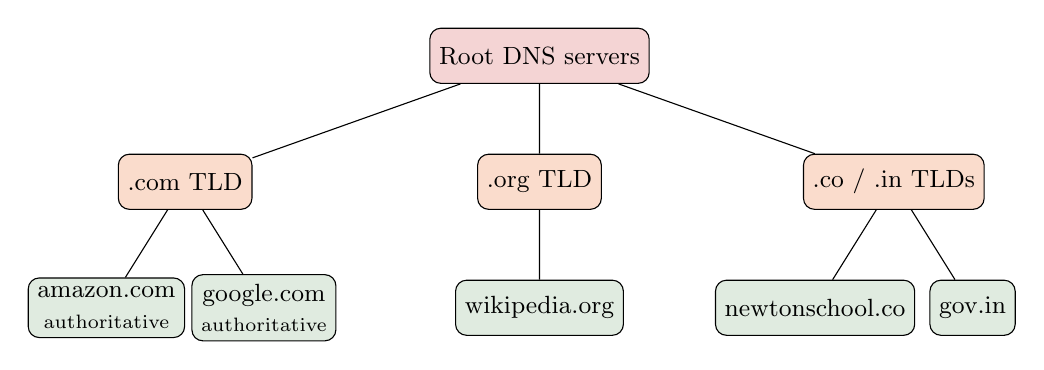
\begin{tikzpicture}[level distance=16mm,
  level 1/.style={sibling distance=45mm},
  level 2/.style={sibling distance=20mm},
  every node/.style={draw,rounded corners,font=\small,align=center,minimum height=7mm}]
  \node[fill=cnred!20] {Root DNS servers}
    child {node[fill=cnorange!20] {.com TLD}
      child {node[fill=cngreen!15] {amazon.com\\\scriptsize authoritative}}
      child {node[fill=cngreen!15] {google.com\\\scriptsize authoritative}}}
    child {node[fill=cnorange!20] {.org TLD}
      child {node[fill=cngreen!15] {wikipedia.org}}}
    child {node[fill=cnorange!20] {.co / .in TLDs}
      child {node[fill=cngreen!15] {newtonschool.co}}
      child {node[fill=cngreen!15] {gov.in}}};
\end{tikzpicture}
\end{center}

\section{Classes of DNS servers}
\subsection{Root DNS servers}
\begin{itemize}
  \item The top of the tree. About \textbf{1000+ instances} worldwide (13 logical root ``names'', copied many times using anycast).
  \item They don't know \texttt{amazon.com}'s IP; they \textbf{provide the IPs of TLD servers} (``ask the .com servers'').
\end{itemize}
\subsection{TLD (Top-Level Domain) servers}
\begin{itemize}
  \item Handle domains such as \textbf{.com, .org, .edu} and country codes (\textbf{.in, .jp}, \ldots).
  \item Maintained by \textbf{registries} (e.g.\ \textbf{Verisign} for .com).
  \item \textbf{Provide the IPs of authoritative servers} (``ask amazon.com's own servers'').
\end{itemize}
\subsection{Authoritative DNS servers}
\begin{itemize}
  \item \textbf{Hold the actual DNS records} for an organisation (e.g.\ \texttt{amazon.com}, \texttt{newtonschool.co}).
  \item \textbf{Map hostnames $\to$ IP addresses} --- they give the final answer.
  \item Can be run by the organisation itself or by a provider (e.g.\ AWS Route 53).
\end{itemize}

\subsection{Local DNS servers (resolvers)}
\begin{itemize}
  \item \textbf{Not part of the hierarchy}, but central to DNS operation at scale.
  \item Provided by \textbf{ISPs} (residential and institutional) --- or public ones like 8.8.8.8.
  \item Acts as a \textbf{proxy}: takes your query and forwards it into the hierarchy for you.
  \item Usually \textbf{close to the client} (on the LAN or a few hops away).
  \item Caches answers, so popular names (google.com) are answered instantly.
\end{itemize}

\section{How a DNS lookup works}
Example: resolving \texttt{www.amazon.com}.
\begin{enumerate}
  \item Client (via local resolver) contacts a \textbf{Root} server $\to$ gets IP addresses of the \textbf{.com TLD} servers.
  \item Contacts the \textbf{.com TLD} server $\to$ gets the IP of the \textbf{authoritative} server for \texttt{amazon.com}.
  \item Contacts the \textbf{authoritative} server for \texttt{amazon.com} $\to$ gets the \textbf{IP of www.amazon.com}.
\end{enumerate}

\begin{center}
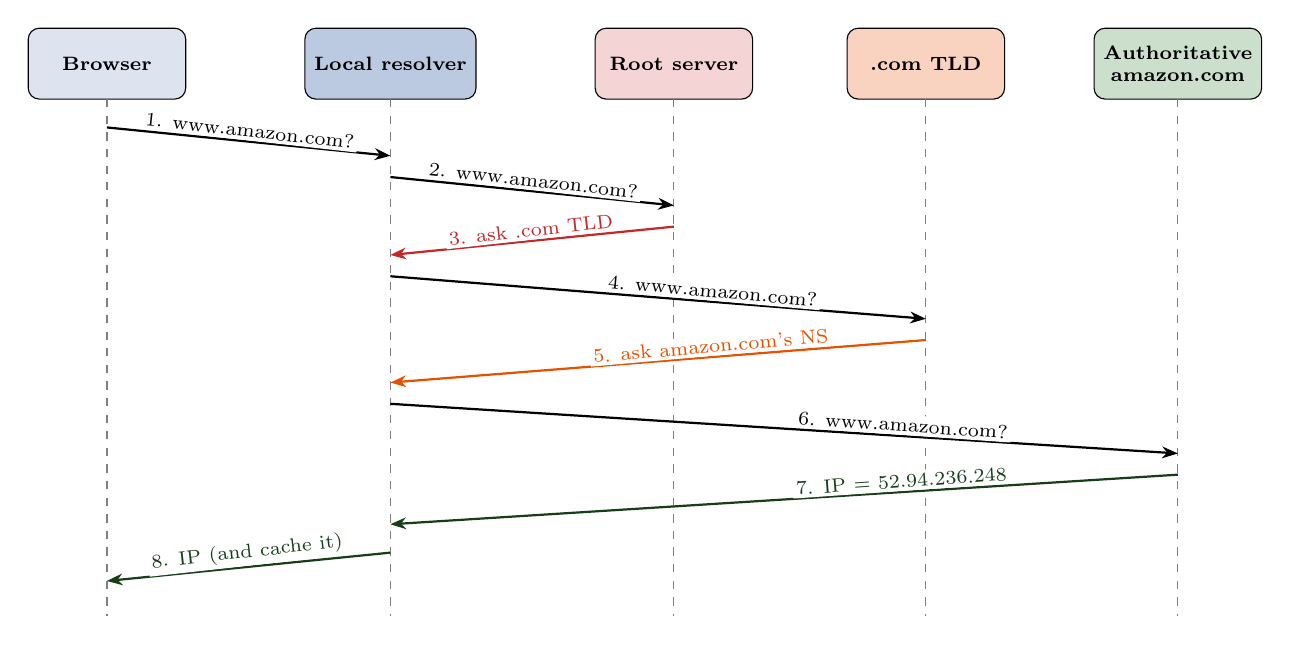
\begin{tikzpicture}[yscale=0.9]
  \foreach \x/\n/\c in {0/Browser/cnblue!15,3.6/Local resolver/cnblue!30,7.2/Root server/cnred!20,10.4/.com TLD/cnorange!25,13.6/Authoritative\\amazon.com/cngreen!25}
    \node[draw,rounded corners,fill=\c,font=\scriptsize\bfseries,align=center,minimum width=20mm,minimum height=9mm] at (\x,0.4) {\n};
  \foreach \x in {0,3.6,7.2,10.4,13.6} \draw[dashed,gray] (\x,-0.1) -- (\x,-7.4);
  \draw[msg] (0,-0.5) -- node[above]{\scriptsize 1. www.amazon.com?} (3.6,-0.9);
  \draw[msg] (3.6,-1.2) -- node[above]{\scriptsize 2. www.amazon.com?} (7.2,-1.6);
  \draw[msg,cnred] (7.2,-1.9) -- node[above]{\scriptsize 3. ask .com TLD} (3.6,-2.3);
  \draw[msg] (3.6,-2.6) -- node[above,pos=0.6]{\scriptsize 4. www.amazon.com?} (10.4,-3.2);
  \draw[msg,cnorange] (10.4,-3.5) -- node[above,pos=0.4]{\scriptsize 5. ask amazon.com's NS} (3.6,-4.1);
  \draw[msg] (3.6,-4.4) -- node[above,pos=0.65]{\scriptsize 6. www.amazon.com?} (13.6,-5.1);
  \draw[msg,cngreen!50!black] (13.6,-5.4) -- node[above,pos=0.35]{\scriptsize 7. IP = 52.94.236.248} (3.6,-6.1);
  \draw[msg,cngreen!50!black] (3.6,-6.5) -- node[above]{\scriptsize 8. IP (and cache it)} (0,-6.9);
\end{tikzpicture}
\end{center}

\textbf{Lecture example:} the user types \texttt{newtonschool.co}. The resolver asks the root (``what is the name server for .co?'' $\to$ ``try 120.x.x.x''), then the .co TLD server (``what is the authoritative DNS for newtonschool.co?'' $\to$ ``try 80.x.x.x''), then the authoritative server (``what is the IP for newtonschool.co?'' $\to$ ``\textbf{99.83.190.102}''). The resolver returns that IP to the browser.

\begin{examtip}
Who gives what? \textbf{Root} $\to$ address of TLD server. \textbf{TLD} $\to$ address of authoritative server. \textbf{Authoritative} $\to$ the final IP address. \textbf{Local resolver} $\to$ does all the asking for you and caches the result. DNS mostly runs over \textbf{UDP port 53}.
\end{examtip}

\section{Demo: \texttt{nslookup}}
\begin{lstlisting}
$ nslookup google.com
Server:   192.168.1.1        <- your local DNS resolver
Address:  192.168.1.1#53

Non-authoritative answer:    <- came from the resolver's cache
Name:     google.com
Address:  142.250.183.14
\end{lstlisting}
``Non-authoritative'' means the answer came from a cache, not straight from Google's authoritative server.

\section{Demo: creating DNS records in AWS Route 53}
\textbf{Amazon Route 53} is AWS's DNS service (named after DNS's port, 53). You create a \textbf{hosted zone} for your domain; Route 53 then acts as the \textbf{authoritative DNS server} for it. Inside the zone you add records, e.g.:
\begin{center}
\begin{tabular}{>{\ttfamily}l l >{\ttfamily}l}
\toprule
\textrm{Name} & Type & \textrm{Value} \\
\midrule
example.com & A & 203.0.113.10 \\
www.example.com & CNAME & example.com \\
example.com & MX & 10 mail.example.com \\
\bottomrule
\end{tabular}
\end{center}

\section{Other topics in this slide deck}
The Lecture 8 deck also contained revision and extension slides. The important ones are summarised here. (UDP, port types, PAT and QUIC slides from this deck are covered in Lecture 9.)

\subsection{The Socket API}
The \textbf{Socket API} is a toolkit that lets applications talk to the \textbf{transport layer}. It is the bridge between your app and protocols like \textbf{TCP and UDP}.
\begin{center}
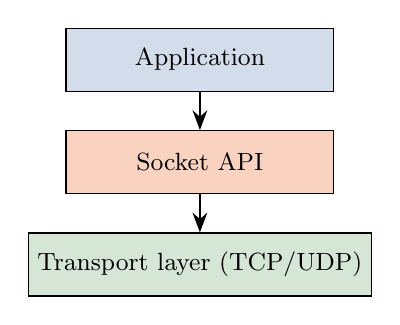
\begin{tikzpicture}[b/.style={draw,minimum width=34mm,minimum height=8mm,font=\small}]
  \node[b,fill=cnblue!20] (a) at (0,0) {Application};
  \node[b,fill=cnorange!25] (s) at (0,-1.3) {Socket API};
  \node[b,fill=cngreen!20] (t) at (0,-2.6) {Transport layer (TCP/UDP)};
  \draw[arr] (a) -- (s); \draw[arr] (s) -- (t);
\end{tikzpicture}
\end{center}

\subsection{HTTP recap}
HTTP is a \textbf{stateless} protocol over TCP. Stages of an HTTP transaction: \textbf{connection $\to$ request $\to$ response $\to$ close}. Each request is independent; the server keeps no memory of earlier requests. (Full details in Lecture 5.)

\subsection{APIs}
\begin{itemize}
  \item \textbf{Client--server paradigm:} client sends a query; server fetches data from a database and responds.
  \item An \textbf{API (Application Programming Interface)} is a set of protocols, routines and tools that let different software systems communicate over a network. It defines \textbf{how components should interact} --- a structured way to send and receive data.
  \item \textbf{Jeff Bezos's API mandate (2002, paraphrased):} all Amazon teams must expose their data and functionality through \textbf{service interfaces}; teams may communicate \textbf{only} through these interfaces over the network; technology doesn't matter; every interface must be designed to be \textbf{externalizable} (usable by outsiders); anyone who doesn't do this will be fired. This thinking later made AWS possible.
  \item \textbf{Examples:} the \textbf{Google Maps API} powers location-based and delivery apps; \textbf{weather APIs} provide forecasts, real-time and historical data (usually JSON or XML) to travel apps (Kayak, AccuWeather) and smart-home devices (Nest).
\end{itemize}

\subsection{Classical ciphers}
A \textbf{cipher} is any method of transforming a message to conceal its meaning.

\textbf{Caesar cipher:} Julius Caesar sent messages through messengers, so he shifted every letter by a fixed number (e.g.\ 3): A$\to$D, B$\to$E, \ldots, Z$\to$C.
\begin{lstlisting}
Plain:  Raj never catches the train. Simran was sad!
Shift 3
Cipher: Udm qhyhu fdwfkhv wkh wudlq. Vlpudq zdv vdg!
\end{lstlisting}

\begin{center}
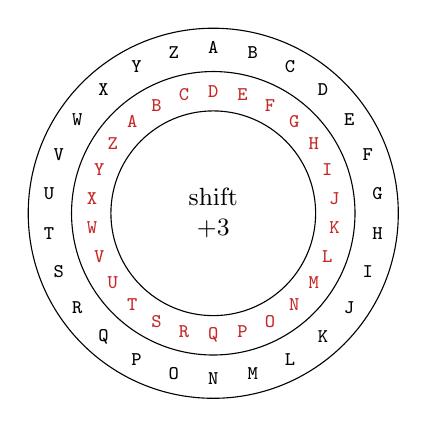
\begin{tikzpicture}
  \foreach \i in {0,...,25} {
    \pgfmathsetmacro{\ang}{90-\i*360/26}
    \node[font=\scriptsize\ttfamily] at (\ang:2.1) {\char\numexpr65+\i\relax};
    \pgfmathtruncatemacro{\j}{mod(\i+3,26)}
    \node[font=\scriptsize\ttfamily,cnred] at (\ang:1.55) {\char\numexpr65+\j\relax};
  }
  \draw (0,0) circle (2.35); \draw (0,0) circle (1.8); \draw (0,0) circle (1.3);
  \node[align=center,font=\small] at (0,0) {shift\\$+3$};
\end{tikzpicture}
\end{center}
Outer ring = plain letter, inner ring = cipher letter.

\begin{workedex}[Substitution cipher puzzle from the slides]
Ciphertext: \texttt{Gztkliv rsyz srrbz yrz dviv ufjk} (shift unknown). Since there are only 26 possible shifts, \textbf{brute force} them all:
\begin{lstlisting}[language=Python]
s = "Gztkliv rsyz srrbz yrz dviv ufjk"
for k in range(26):
    print(k, "".join(chr((ord(c.lower())-97-k) % 26 + 97)
                     if c.isalpha() else c for c in s))
\end{lstlisting}
At shift \textbf{17} you get: \textbf{``picture abhi baaki hai mere dost''}. Lesson: shift ciphers are trivially breakable --- real security needs modern cryptography.
\end{workedex}

\subsection{Alice, Bob and Mallory (since 1978)}
In cryptography stories, \textbf{Alice} and \textbf{Bob} want to talk securely, and \textbf{Mallory} is the malicious attacker in the middle.

\textbf{Man-in-the-middle (MITM) attack:} the attacker secretly sits between a user and the website they are visiting, relaying (and possibly reading or changing) everything.
\begin{center}
\begin{tikzpicture}
  \node[host] (a) at (0,0) {Alice\\\scriptsize(user)};
  \node[draw,fill=cnred!25,minimum width=16mm,minimum height=10mm,align=center] (m) at (4.5,0) {Mallory\\\scriptsize(attacker)};
  \node[srv] (b) at (9,0) {Bob\\\scriptsize(website)};
  \draw[darr,cnred] (a) -- (m); \draw[darr,cnred] (m) -- (b);
  \draw[dashed,gray,darr] (a.north) to[bend left=25] node[above,font=\scriptsize]{what Alice thinks is happening} (b.north);
\end{tikzpicture}
\end{center}

\textbf{The challenge of communicating secrets in public} --- three threats:
\begin{center}
\begin{tabular}{lll}
\toprule
Threat & What Mallory does & Defended by \\
\midrule
Eavesdropping & reads the messages & Confidentiality (encryption) \\
Tampering & changes the messages & Integrity (MACs / hashes) \\
Impersonation & pretends to be Bob & Authentication (certificates) \\
\bottomrule
\end{tabular}
\end{center}

\subsection{How TLS gets added on top of TCP (detailed steps)}
After the TCP 3-way handshake, TLS runs its own handshake:
\begin{enumerate}
  \item \textbf{ClientHello:} supported TLS versions, list of cipher suites, a random number (\texttt{client\_random}), optionally the server name. \emph{``Here are the languages I speak. Can we talk securely?''}
  \item \textbf{ServerHello:} chosen TLS version, selected cipher suite, its own random number (\texttt{server\_random}), its \textbf{digital certificate}. \emph{``I'll speak this language. Here's my ID.''}
  \item \textbf{Certificate verification (client side):} is the certificate valid and trusted (via a CA)? Does the hostname match? Is it unexpired and not revoked? \emph{Like checking that a driver's licence is real and matches the person.}
  \item \textbf{Pre-master secret:} the client generates a temporary shared value, encrypts it with the server's \textbf{public key} and sends it. Only the server can decrypt it (only it has the private key).
  \item \textbf{Key derivation (both sides):} from pre-master secret + \texttt{client\_random} + \texttt{server\_random}, both derive the \textbf{same symmetric session key}.
  \item \textbf{Finished messages:} each side sends a ``Finished'' message encrypted with the new key. Now both know the connection is secure --- the handshake is complete.
\end{enumerate}

\begin{recap}
\begin{itemize}
  \item DNS = name $\to$ IP. Distributed, hierarchical database; no single server knows everything.
  \item Records: A (IPv4), AAAA (IPv6), MX (mail), NS (name servers), CNAME (alias), TXT.
  \item Root ($\sim$1000+ instances) $\to$ IPs of TLD servers. TLD (.com/.org/.in; run by registries like Verisign) $\to$ IPs of authoritative. Authoritative $\to$ final IP.
  \item Local resolver (ISP): not in hierarchy, acts as proxy, close to client, caches.
  \item \texttt{nslookup} to query; Route 53 = AWS's authoritative DNS (hosted zones, records).
  \item Extras: Socket API; APIs \& Bezos mandate; Caesar/shift cipher (brute force: 26 tries); MITM; 6-step TLS.
\end{itemize}
\end{recap}

\chapter{Lecture 9 --- The Transport Layer: Multiplexing, Ports, UDP and the TCP Connection}

\begin{keyidea}[The one idea from this lecture]
The network layer (IP) delivers data to the right \textbf{computer}. The transport layer delivers it to the right \textbf{program} on that computer, using \textbf{port numbers}. It offers two services: \textbf{UDP} --- fast, simple, no guarantees; and \textbf{TCP} --- connection-based, ordered and reliable (3-way handshake, sequence numbers, ACKs, retransmission).
\end{keyidea}

\section{Recap: DNS lookup}
Example \texttt{www.amazon.com}: (1) Root server $\to$ IPs of .com TLD servers; (2) .com TLD $\to$ IP of amazon.com's authoritative server; (3) authoritative server $\to$ IP of www.amazon.com. Now we go one layer down: \textbf{Layer 4}.

\section{Layer 4 --- the transport layer}
\begin{itemize}
  \item Implemented \textbf{only in the end devices} (sender and receiver).
  \item \textbf{Routers only process network-layer} information; they \textbf{ignore} TCP/UDP segment fields completely.
  \item The transport layer converts application \textbf{messages} into \textbf{segments}.
  \item Transport layer = communication between \textbf{processes}; network layer = communication between \textbf{hosts}.
\end{itemize}

\begin{center}
\begin{tikzpicture}[b/.style={draw,minimum width=16mm,minimum height=5.5mm,font=\scriptsize}]
  \foreach \x/\name/\top in {0/Sender/5,4/Router/3,8/Router/3,12/Receiver/5} {
    \node[font=\small\bfseries] at (\x,0.5) {\name};
    \ifnum\top=5
      \node[b,fill=cnblue!20] at (\x,0) {Application};
      \node[b,fill=cngreen!30] at (\x,-0.55) {Transport};
    \fi
    \node[b,fill=cnorange!25] at (\x,-1.1) {Network};
    \node[b,fill=cnpurple!15] at (\x,-1.65) {Link};
    \node[b,fill=gray!20] at (\x,-2.2) {Physical};
  }
  \draw[thick] (0.8,-2.2) -- (3.2,-2.2); \draw[thick] (4.8,-2.2) -- (7.2,-2.2); \draw[thick] (8.8,-2.2) -- (11.2,-2.2);
  \draw[dashed,cngreen!60!black,darr] (0.8,-0.55) -- node[above,font=\scriptsize]{transport: process-to-process (routers don't look)} (11.2,-0.55);
\end{tikzpicture}
\end{center}

\section{Ports and sockets}
\begin{analogy}[The apartment building]
To send a letter to a friend in a large apartment building you need \textbf{both} the \textbf{building's street address} (1 Infinite Loop) \textbf{and} the \textbf{apartment number} (\#443). Without both, the letter gets lost.
\end{analogy}
\begin{itemize}
  \item \textbf{IP address} = the computer's ``street address'' (e.g.\ 172.217.167.78).
  \item \textbf{Port number} = the application's ``apartment number'' (e.g.\ 443).
  \item \textbf{IP address + port number = socket} --- a unique endpoint (doorway) for a conversation.
\end{itemize}

\begin{center}
\begin{tikzpicture}
  \node[draw,rounded corners,fill=cnblue!10,minimum width=44mm,minimum height=12mm,align=center] (l) at (0,0) {Your laptop\\\ttfamily\small 192.168.1.5:52344};
  \node[draw,rounded corners,fill=cngreen!12,minimum width=44mm,minimum height=12mm,align=center] (g) at (10,0) {Google server\\\ttfamily\small 172.217.167.78:443};
  \draw[darr] (l) -- node[above,font=\small]{TCP connection} node[below=2mm,font=\scriptsize,align=center]{random client port\\$\leftrightarrow$ well-known server port} (g);
\end{tikzpicture}
\end{center}
To see open sockets on Linux: \texttt{netstat -tnlp} (\texttt{t}=TCP, \texttt{n}=numeric, \texttt{l}=listening, \texttt{p}=program).

\subsection{Types of port numbers}
Port numbers are 16-bit (0--65535), in three ranges:
\begin{center}
\begin{tikzpicture}
  \fill[cnblue!35] (-1,2) -- (1,2) -- (0,3.3) -- cycle; \node[font=\scriptsize\bfseries] at (0,2.35) {Well-known};
  \fill[cnblue!30] (-2,1) -- (2,1) -- (1,2) -- (-1,2) -- cycle; \node[font=\small\bfseries] at (0,1.5) {Registered};
  \fill[cnblue!15] (-3,0) -- (3,0) -- (2,1) -- (-2,1) -- cycle; \node[font=\small\bfseries] at (0,0.5) {Dynamic / Private};
  \node[font=\scriptsize,anchor=west] at (1.4,2.5) {0--1023};
  \node[font=\scriptsize,anchor=west] at (2.3,1.5) {1024--49151};
  \node[font=\scriptsize,anchor=west] at (3.2,0.5) {49152--65535};
\end{tikzpicture}
\end{center}
\begin{enumerate}
  \item \textbf{Well-known ports (0--1023):} reserved for standard services --- HTTP \textbf{80}, HTTPS \textbf{443}, FTP \textbf{21}, DNS \textbf{53}, SSH \textbf{22} (also SMTP 25, POP3 110, IMAP 143).
  \item \textbf{Registered ports (1024--49151):} used by third-party apps/vendors --- MySQL \textbf{3306}, PostgreSQL \textbf{5432}, Docker \textbf{2375}.
  \item \textbf{Dynamic / private ports (49152--65535):} temporarily assigned by the OS for \textbf{client-side} connections (e.g.\ when your browser opens a connection). Also called \emph{ephemeral} ports.
\end{enumerate}

\section{Multiplexing and demultiplexing}
\begin{itemize}
  \item \textbf{Multiplexing (sender side):} collecting data from \textbf{many application processes}, adding headers (with port numbers), and sending it all through the network.
  \item \textbf{Demultiplexing (receiver side):} delivering each received segment to the \textbf{correct application process}, by checking the \textbf{destination port number}.
\end{itemize}
\begin{analogy}[Letters in a courier box]
Many letters (segments) travel together in one courier box (the IP connection to your computer). At the destination, the box is opened and each letter is handed to the right person based on the name on its envelope (the port number).
\end{analogy}

\begin{center}
\begin{tikzpicture}
  \node[font=\small\bfseries] at (-0.5,1.6) {Multiplexing};
  \foreach \y/\n/\p in {1/HTTP/80,0.33/DNS/53,-0.33/SSH/22,-1/Other/{*}} {
    \node[font=\scriptsize,anchor=east] at (-1.2,\y) {\n};
    \draw[thick,cnblue] (-1.1,\y) .. controls (0,\y) and (0.5,0) .. (1.5,0);
    \node[font=\tiny] at (-0.6,\y+0.13) {\p};
  }
  \draw[line width=4pt,cnblue!70] (1.5,0) -- node[above,font=\scriptsize,text=black]{one network link} (5.5,0);
  \node[font=\small\bfseries] at (7.0,1.6) {Demultiplexing};
  \foreach \y/\n in {1/HTTP,0.33/DNS,-0.33/SSH,-1/Other} {
    \draw[thick,cngreen!60!black,->] (5.5,0) .. controls (6.5,0) and (7,\y) .. (7.8,\y);
    \node[font=\scriptsize,anchor=west] at (7.9,\y) {\n};
  }
  \node[font=\scriptsize,align=center] at (6.9,-1.6) {by destination port};
\end{tikzpicture}
\end{center}

Example: a laptop runs a browser, an email app and a music app at the same time. Replies from a web server (port 80), mail server (port 25) and music server arrive on the same network card; the transport layer hands each to the right app using the port.

\section{Port Address Translation (PAT)}
\begin{itemize}
  \item \textbf{PAT} is a type of \textbf{NAT} (Network Address Translation) that lets \textbf{many devices on a private network share a single public IP address}.
  \item Instead of giving every device its own public IP, PAT uses \textbf{unique port numbers} to track each connection. This \textbf{conserves public IP addresses}.
  \item PAT rewrites \textbf{both the IP address and the port number}. Each internal connection gets: shared public IP + a unique port (per session).
  \item The router keeps a \textbf{translation table}; when a reply comes back to that port, it knows which internal device and port to forward it to.
  \item So dozens or hundreds of devices can use the internet at the same time through one public IP.
\end{itemize}

\begin{center}
\begin{tikzpicture}
  \node[host,font=\scriptsize] (a) at (0,1.4) {Laptop\\192.168.0.2:1234};
  \node[host,font=\scriptsize] (b) at (0,0) {Phone\\192.168.0.3:3000};
  \node[host,font=\scriptsize] (c) at (0,-1.4) {Smart TV\\192.168.0.4:2001};
  \node[rtr,minimum size=12mm,font=\scriptsize,align=center] (r) at (4,0) {PAT\\router};
  \node[font=\scriptsize] at (4,-0.95) {public IP 203.0.113.5};
  \foreach \d in {a,b,c} \draw[arr] (\d) -- (r);
  \node[srv,font=\scriptsize] (s1) at (8,1.4) {Server A};
  \node[srv,font=\scriptsize] (s2) at (8,0) {Server B};
  \node[srv,font=\scriptsize] (s3) at (8,-1.4) {Server C};
  \draw[arr] (r) -- node[above,sloped,font=\tiny]{:45000} (s1);
  \draw[arr] (r) -- node[above,font=\tiny]{:45001} (s2);
  \draw[arr] (r) -- node[below,sloped,font=\tiny]{:45002} (s3);
\end{tikzpicture}
\end{center}
\begin{center}
\begin{tabular}{>{\ttfamily}l >{\ttfamily}l}
\toprule
\textrm{Inside (private IP:port)} & \textrm{Outside (public IP:port)} \\
\midrule
192.168.0.2:1234 & 203.0.113.5:45000 \\
192.168.0.3:3000 & 203.0.113.5:45001 \\
192.168.0.4:2001 & 203.0.113.5:45002 \\
\bottomrule
\end{tabular}
\end{center}

\section{Transport layer protocols: UDP and TCP}

\subsection{UDP --- User Datagram Protocol}
\begin{analogy}[``Who cares? UDP just sent it faster!'']
The receiver asks ``Are you getting all of this?'' and UDP replies ``Who cares? I just sent it faster!'' UDP fires packets off without checking they arrived.
\end{analogy}
\begin{itemize}
  \item \textbf{Connectionless:} no handshake --- just send.
  \item \textbf{No guarantees:} no acknowledgements, no retransmission, no ordering.
  \item \textbf{Tiny header (8 bytes) $\Rightarrow$ low overhead, very fast.}
\end{itemize}

\textbf{UDP segment format} (32 bits wide):
\begin{center}
\begin{tikzpicture}[f/.style={draw,minimum height=8mm,font=\small,align=center}]
  \node[font=\scriptsize] at (3,0.65) {$\longleftarrow$ 32 bits $\longrightarrow$};
  \node[f,minimum width=30mm,fill=cnblue!15] at (1.5,0) {source port \#};
  \node[f,minimum width=30mm,fill=cnblue!15] at (4.5,0) {dest port \#};
  \node[f,minimum width=30mm,fill=cnorange!15] at (1.5,-0.8) {length};
  \node[f,minimum width=30mm,fill=cnorange!15] at (4.5,-0.8) {checksum};
  \node[f,minimum width=60mm,minimum height=16mm,fill=cngreen!10] at (3,-2.0) {application data\\(payload)};
  \node[font=\scriptsize,anchor=west,align=left] at (6.3,-0.8) {length in bytes of UDP\\segment, incl.\ header};
\end{tikzpicture}
\end{center}

\subsection{Where UDP shines --- use cases}
\begin{itemize}
  \item \textbf{DNS:} a single short question and answer; if the reply is lost, just ask again. (Lookup: user $\to$ local DNS $\to$ root $\to$ TLD $\to$ authoritative, e.g.\ \texttt{newtonschool.co} $\to$ 99.83.190.102.)
  \item \textbf{Live video streaming} (cricket, news, gaming streams): unlike buffered YouTube videos, live streams prioritise \textbf{speed}. UDP sends frames quickly; if some are lost, they are \textbf{skipped} to avoid lag. Goal: smooth, instant flow.
  \item \textbf{Online gaming:} real-time speed matters more than perfect accuracy. Late data is useless --- better to lose a packet than wait for it.
  \item \textbf{SNMP} (Simple Network Management Protocol): small, quick status requests (``is this router online?''); if a reply is lost it simply retries --- efficient for large networks.
  \item \textbf{TFTP} (Trivial File Transfer Protocol): small config/boot files on trusted local networks, where speed and simplicity matter more than reliability --- avoids TCP's start-up overhead.
  \item \textbf{DHCP} (Dynamic Host Configuration Protocol): quickly assigns IP addresses when a device joins a network with one-time request/response messages; the application handles any needed reliability.
\end{itemize}
Lab demo: a \textbf{UDP chat using \texttt{nc}} (netcat): \texttt{nc -u -l 9999} on one side, \texttt{nc -u <ip> 9999} on the other.

\subsection{QUIC --- Quick UDP Internet Connections}
\begin{itemize}
  \item A modern transport protocol built \textbf{on top of UDP}, designed by \textbf{Google}.
  \item Used by \textbf{HTTP/3} to make browsing faster and more secure: combines UDP's speed with TCP-like reliability.
  \item Avoids TCP's slow handshakes, handles packet loss efficiently, has \textbf{built-in TLS encryption}, faster connection setup and \textbf{stream multiplexing}.
  \item Used by Google, YouTube and Facebook.
\end{itemize}

\section{TCP --- Transmission Control Protocol}
TCP is \textbf{connection-oriented} and \textbf{reliable}: before any data is sent, the two sides set up a connection with the \textbf{3-way handshake}.

\subsection{The TCP 3-way handshake}
Story: your browser (client) connecting to a Google server (listening on port 443).

\begin{center}
\begin{tikzpicture}
  \node[draw,fill=cnblue!20,font=\bfseries] at (0,0.5) {Client (browser)};
  \node[draw,fill=cngreen!20,font=\bfseries] at (8,0.5) {Server (Google :443)};
  \lifelines{0}{8}{0}{-4.2}
  \draw[msg,cnblue] (0,-0.4) -- node[above,font=\small,sloped]{\textbf{SYN}, seq = 100} (8,-1.2);
  \draw[msg,cngreen!60!black] (8,-1.6) -- node[above,font=\small,sloped]{\textbf{SYN-ACK}, seq = 350, ack = 101} (0,-2.4);
  \draw[msg,cnblue] (0,-2.8) -- node[above,font=\small,sloped]{\textbf{ACK}, ack = 351} (8,-3.6);
  \node[font=\small\bfseries,cnred] at (4,-4.3) {ESTABLISHED --- data can flow};
\end{tikzpicture}
\end{center}

\begin{enumerate}
  \item \textbf{The ring --- SYN} (``synchronize''): \emph{``Hey, are you there? I'd like to talk. I'll start numbering my sentences at 100.''}
  \item \textbf{The ``Hello?'' --- SYN-ACK:} the server does two things at once: \emph{``Yes, I'm here! I ACKnowledge you start at 100. And I'll SYNchronize my side starting at 350. Ready?''}
  \item \textbf{The ``I'm here!'' --- ACK:} \emph{``Got it! I acknowledge you start at 350. Let's talk!''} $\Rightarrow$ connection \textbf{ESTABLISHED}.
\end{enumerate}

\subsection{TCP connection teardown (4-way handshake)}
TCP says goodbye politely:
\begin{center}
\begin{tikzpicture}
  \node[draw,fill=cnblue!20,font=\bfseries] at (0,0.5) {Client};
  \node[draw,fill=cngreen!20,font=\bfseries] at (8,0.5) {Server};
  \lifelines{0}{8}{0}{-4.6}
  \draw[msg,cnblue] (0,-0.3) -- node[above,sloped,font=\small]{1. \textbf{FIN} (``I have to go'')} (8,-1.0);
  \draw[msg,cngreen!60!black] (8,-1.3) -- node[above,sloped,font=\small]{2. \textbf{ACK} (``Okay'')} (0,-2.0);
  \node[font=\scriptsize,align=right,anchor=east] at (7.9,-2.4) {server finishes sending remaining data};
  \draw[msg,cngreen!60!black] (8,-2.8) -- node[above,sloped,font=\small]{3. \textbf{FIN} (``I'm done too'')} (0,-3.5);
  \draw[msg,cnblue] (0,-3.8) -- node[above,sloped,font=\small]{4. \textbf{ACK} (``Bye'')} (8,-4.5);
\end{tikzpicture}
\end{center}

\subsection{Sequence numbers $\Rightarrow$ ordered delivery}
Segments can take different routes and \textbf{arrive out of order}. Imagine reading: ``the mat.'' ``The cat'' ``sat on'' --- confusing! TCP numbers every segment (using the sequence numbers agreed in the handshake). If segment \#3 arrives before \#2, the receiver \textbf{waits for \#2} and then hands the data to the application in the correct order: ``The cat sat on the mat.''

\subsection{Acknowledgements and retransmission}
On a phone call you know the other person heard you when they say ``hmm'' or ``achcha''. TCP does the same:
\begin{itemize}
  \item When the server receives bytes 101--200, it sends back an \textbf{ACK} saying \emph{``I've received everything up to 200; send 201 next''} (ack number = \textbf{next expected byte}).
  \item If the sender gets \textbf{no ACK within a certain time} (timeout), it assumes the data was lost and \textbf{retransmits} it.
\end{itemize}

\begin{center}
\begin{tikzpicture}
  \node[font=\bfseries] at (0,0.4) {Sender}; \node[font=\bfseries] at (7,0.4) {Receiver};
  \lifelines{0}{7}{0}{-4.4}
  \draw[msg] (0,-0.3) -- node[above,sloped,font=\scriptsize]{bytes 101--200} (7,-0.9);
  \draw[msg,cngreen!60!black] (7,-1.1) -- node[above,sloped,font=\scriptsize]{ACK 201} (0,-1.7);
  \draw[msg] (0,-1.9) -- (4.2,-2.25); \node[cnred,font=\bfseries] at (4.4,-2.27) {$\times$};
  \node[font=\scriptsize,cnred] at (4.6,-2.6) {lost};
  \draw[decorate,decoration={brace,mirror,amplitude=4pt}] (-0.15,-1.9) -- (-0.15,-3.3) node[midway,left=5pt,font=\scriptsize]{timeout};
  \draw[msg] (0,-3.4) -- node[above,sloped,font=\scriptsize]{bytes 201--300 (retransmitted)} (7,-4.0);
  \draw[msg,cngreen!60!black] (7,-4.1) -- node[below,sloped,font=\scriptsize]{ACK 301} (0,-4.6);
\end{tikzpicture}
\end{center}

\subsection{TCP segment header (preview)}
\begin{center}
\begin{tikzpicture}[f/.style={draw,minimum height=7mm,font=\scriptsize,align=center}]
  \node[font=\scriptsize] at (4,0.6) {$\longleftarrow$ 32 bits $\longrightarrow$};
  \node[f,minimum width=40mm,fill=cnblue!15] at (2,0) {Source port (16)};
  \node[f,minimum width=40mm,fill=cnblue!15] at (6,0) {Destination port (16)};
  \node[f,minimum width=80mm,fill=cnorange!15] at (4,-0.7) {Sequence number (32)};
  \node[f,minimum width=80mm,fill=cnorange!15] at (4,-1.4) {Acknowledgment number (32)};
  \node[f,minimum width=12mm,fill=cnpurple!15] at (0.6,-2.1) {Data\\[-3pt]offset};
  \node[f,minimum width=10mm,fill=gray!15] at (1.7,-2.1) {Rsvd};
  \node[f,minimum width=18mm,fill=cnred!15] at (3.1,-2.1) {Flags\\[-3pt]SYN ACK FIN\ldots};
  \node[f,minimum width=40mm,fill=cngreen!15] at (6,-2.1) {Window size (16)};
  \node[f,minimum width=40mm,fill=cnpurple!10] at (2,-2.8) {Checksum (16)};
  \node[f,minimum width=40mm,fill=cnpurple!10] at (6,-2.8) {Urgent pointer (16)};
  \node[f,minimum width=80mm,fill=white] at (4,-3.5) {Options (variable)};
  \node[f,minimum width=80mm,minimum height=10mm,fill=cngreen!8] at (4,-4.35) {Data (payload)};
\end{tikzpicture}
\end{center}
\begin{center}
\begin{tabularx}{\textwidth}{>{\bfseries}l X}
\toprule
Field & Purpose \\
\midrule
Source port & Port of the sending application. \\
Destination port & Port of the receiving application. \\
Sequence number & Identifies the bytes in this segment, so data can be put in order. \\
Acknowledgment number & Confirms receipt; = the \textbf{next expected} sequence number. \\
Data offset & Length of the TCP header in 32-bit words. \\
Control flags & Control bits such as \textbf{SYN, ACK, FIN} (also RST, PSH, URG). \\
Window size & Receiver's available buffer --- used for \textbf{flow control} (Lecture 10). \\
Checksum & Detects corruption --- data integrity. \\
Urgent pointer & If URG flag is set: offset from the sequence number to the last urgent byte. \\
\bottomrule
\end{tabularx}
\end{center}

\section{Speed vs reliability --- the UDP/TCP trade-off}
\begin{center}
\begin{tikzpicture}
  \begin{scope}
    \node[font=\bfseries,fill=cnblue!40,text=white,minimum width=50mm] at (2,0.9) {UDP};
    \lifelines{0}{4}{0.5}{-2.4}
    \foreach \y in {0.2,-0.5,-1.2,-1.9} \draw[msg] (0,\y) -- (4,\y-0.3);
    \node[font=\scriptsize] at (2,-2.7) {just send, no setup, no ACKs};
  \end{scope}
  \begin{scope}[xshift=7cm]
    \node[font=\bfseries,fill=cnpurple!40,text=white,minimum width=50mm] at (2,0.9) {TCP};
    \lifelines{0}{4}{0.5}{-2.4}
    \draw[msg] (0,0.2) -- node[above,font=\tiny]{SYN} (4,-0.1);
    \draw[msg] (4,-0.2) -- node[above,font=\tiny]{SYN-ACK} (0,-0.5);
    \draw[msg] (0,-0.6) -- node[above,font=\tiny]{ACK} (4,-0.9);
    \draw[msg] (0,-1.2) -- node[above,font=\tiny]{data} (4,-1.5);
    \draw[msg] (4,-1.7) -- node[above,font=\tiny]{ACK} (0,-2.0);
    \node[font=\scriptsize] at (2,-2.7) {handshake, ACKs, retransmissions};
  \end{scope}
\end{tikzpicture}
\end{center}

\begin{center}
\begin{tabularx}{\textwidth}{>{\bfseries}l X X}
\toprule
 & UDP & TCP \\
\midrule
Connection & Connectionless & Connection-oriented (3-way handshake) \\
Reliability & None --- lost data is lost & Reliable --- ACKs + retransmission \\
Ordering & No & Yes (sequence numbers) \\
Header size & 8 bytes & 20+ bytes \\
Speed & Faster, low overhead & Slower, more overhead \\
Flow/congestion control & No & Yes \\
Used by & DNS, live streaming, gaming, SNMP, TFTP, DHCP, QUIC/HTTP3 & HTTP/1.1, HTTP/2, HTTPS, SMTP, IMAP, POP3, SSH, FTP \\
\bottomrule
\end{tabularx}
\end{center}

\begin{recap}
\begin{itemize}
  \item Transport layer lives only in end hosts; routers ignore it. Messages $\to$ segments. Process-to-process.
  \item Socket = IP + port. Ports: well-known 0--1023, registered 1024--49151, dynamic 49152--65535.
  \item Multiplexing (sender gathers from many apps) / demultiplexing (receiver delivers by destination port).
  \item PAT: many private devices share one public IP by using unique ports; rewrites IP and port.
  \item UDP: connectionless, no guarantees, 8-byte header (src port, dst port, length, checksum). Uses: DNS, live video, gaming, SNMP, TFTP, DHCP. QUIC is built on UDP.
  \item TCP: SYN $\to$ SYN-ACK $\to$ ACK; teardown FIN, ACK, FIN, ACK. Sequence numbers for order; ACK = next expected byte; timeout $\Rightarrow$ retransmit.
\end{itemize}
\end{recap}

\chapter{Lecture 10 --- Reliable Data Transfer and TCP Flow Control}

\begin{keyidea}[The one idea from this lecture]
The network underneath is unreliable (packets get lost, corrupted, reordered). TCP builds \textbf{reliability} on top of it using \textbf{checksums} (detect corruption), \textbf{ACKs + timeouts based on RTT} (detect loss), and \textbf{retransmission}. To be efficient it sends many packets at once (\textbf{sliding window}) instead of one at a time (\textbf{stop-and-wait}), and uses \textbf{flow control} so a fast sender doesn't drown a slow receiver. When packets are lost, \textbf{Go-Back-N} resends everything from the lost one; \textbf{Selective Repeat} resends only the lost one.
\end{keyidea}

\section{Layers recap: building reliability from an unreliable channel}
IP (network layer) is \textbf{best effort}: no guarantee of delivery, order or correctness. The transport layer (TCP) turns that into a reliable byte stream for the application.

\begin{center}
\begin{tikzpicture}
  \node[draw,fill=cnblue!15,minimum width=40mm,minimum height=8mm] (a) at (0,0) {Application: wants reliable data};
  \node[draw,fill=cngreen!25,minimum width=40mm,minimum height=8mm] (t) at (0,-1.2) {TCP: reliable data transfer};
  \node[draw,fill=cnred!15,minimum width=40mm,minimum height=8mm] (n) at (0,-2.4) {Unreliable channel (IP)};
  \draw[arr] (a) -- (t); \draw[arr] (t) -- (n);
  \node[right=5mm of n,font=\scriptsize,align=left] {may lose, corrupt,\\reorder packets};
  \node[right=5mm of t,font=\scriptsize,align=left] {checksums, seq numbers,\\ACKs, timers, retransmission};
\end{tikzpicture}
\end{center}

\section{TCP --- Transmission Control Protocol}
\begin{itemize}
  \item \textbf{Establishes a connection} before data transfer (3-way handshake).
  \item Maintains \textbf{data integrity} using \textbf{sequence numbers, acknowledgements and checksums}.
  \item Ensures \textbf{reliable, ordered delivery}, handling any loss.
  \item Handles \textbf{connection teardown} too.
\end{itemize}

\subsection{TCP connection teardown (4-way handshake) --- recap}
\begin{enumerate}
  \item Client sends \textbf{FIN} --- ``I have to go.''
  \item Server replies \textbf{ACK} --- ``Okay.''
  \item When the server has finished sending its remaining data, it sends its own \textbf{FIN} --- ``I'm done too.''
  \item Client sends a final \textbf{ACK} --- ``Bye.''
\end{enumerate}
(In class this was observed in \textbf{Wireshark} using a TCP echo server: you can see SYN, SYN-ACK, ACK, the data with ACKs, then FIN/ACK/FIN/ACK.)

\section{Checksums --- detecting corruption}
TCP aims for reliable transfer, so it needs to \textbf{detect transmission errors} (bits flipped by noise) so that corrupted data can be retransmitted. It uses the \textbf{Internet checksum}: add the data in fixed-size chunks with \textbf{1's complement arithmetic} (any carry out of the top bit is \textbf{wrapped around} and added back), then \textbf{flip all the bits}.

\subsection{Sender (Alice)}
\begin{enumerate}
  \item Split data into chunks (real TCP uses 16-bit words; the lecture uses 8-bit chunks for simplicity).
  \item \textbf{Add} the chunks. If there is a \textbf{carry} out of the leftmost bit, \textbf{add it back} to the result (wrap-around).
  \item Take the \textbf{1's complement} (flip every bit) $\Rightarrow$ this is the checksum.
  \item Send the data \textbf{and} the checksum.
\end{enumerate}

\subsection{Receiver (Bob)}
Bob adds the received data chunks \textbf{and} the received checksum (with wrap-around). If the result is \textbf{all 1s}, the data is correct with high probability. If any bit is 0, an error happened $\Rightarrow$ discard (and it will be retransmitted).

\begin{workedex}[Example 1 --- the lecture's data: $147 + 86$]
Chunk 1 = \texttt{10010011} (147), Chunk 2 = \texttt{01010110} (86).
\begin{lstlisting}
    10010011      (147)
  + 01010110      ( 86)
  ----------
    11101001      (233)  -> fits in 8 bits, no carry this time
\end{lstlisting}
1's complement (flip bits): \texttt{11101001} $\to$ \textbf{checksum = \texttt{00010110}}.

Receiver check:
\begin{lstlisting}
    11101001      (sum of data)
  + 00010110      (checksum received)
  ----------
    11111111      -> all 1s, data is OK
\end{lstlisting}
\textbf{Note:} the lecture slides show this example with a carry (sum \texttt{1 00001001}, checksum \texttt{11110101}). But $147+86 = 233$, which fits in 8 bits, so there is no carry and the correct checksum is \texttt{00010110}. The \emph{method} on the slides is right; Example 2 shows what to do when a carry really happens.
\end{workedex}

\begin{workedex}[Example 2 --- with a carry (wrap-around)]
Chunk 1 = \texttt{10110011} (179), Chunk 2 = \texttt{11100101} (229).
\begin{lstlisting}
      10110011      (179)
    + 11100101      (229)
    ----------
    1 10011000      (408) -> carry-over bit!
Wrap around: add the carry back
      10011000
    +        1
    ----------
      10011001      (sum)
1's complement: 01100110   <- checksum
Receiver: 10011001 + 01100110 = 11111111  -> all 1s
\end{lstlisting}
\end{workedex}

\begin{center}
\begin{tikzpicture}
  \node[draw,fill=cnblue!15,align=center,minimum width=26mm] (s) at (0,0) {Alice\\\scriptsize sum $\to$ wrap $\to$ flip};
  \node[draw,fill=cngreen!15,align=center,minimum width=26mm] (r) at (8,0) {Bob\\\scriptsize sum + checksum};
  \draw[arr] (s) -- node[above,font=\scriptsize]{data + checksum} (r);
  \node[draw,fill=cngreen!30,font=\scriptsize] (ok) at (10.8,0.6) {all 1s $\Rightarrow$ OK};
  \node[draw,fill=cnred!25,font=\scriptsize] (bad) at (10.8,-0.6) {any 0 $\Rightarrow$ error};
  \draw[->] (r) -- (ok); \draw[->] (r) -- (bad);
\end{tikzpicture}
\end{center}

\section{The waiting game: Round Trip Time (RTT)}
Alice sends a segment to Carol and needs a receipt (\textbf{ACK}) to know it arrived. \textbf{How long should she wait before assuming it was lost?} 10 ms? A whole second?

\textbf{RTT (Round Trip Time)} = the total time for a segment to go from Alice to Carol \textbf{plus} the time for Carol's ACK to come back.
\begin{itemize}
  \item TCP measures RTT continuously and sets its \textbf{timeout a bit larger than the RTT}.
  \item Too short a timeout $\Rightarrow$ needless retransmissions. Too long $\Rightarrow$ slow reaction to real loss.
  \item You can see RTT with \texttt{ping}: e.g.\ \texttt{ping newtonschool.co} (nearby server, small RTT) vs \texttt{ping taobao.com} (server in China, much larger RTT, because of distance --- propagation delay!).
\end{itemize}

\begin{center}
\begin{tikzpicture}
  \node[font=\bfseries] at (0,0.4) {Alice}; \node[font=\bfseries] at (6,0.4) {Carol};
  \lifelines{0}{6}{0}{-2.6}
  \draw[msg] (0,-0.2) -- node[above,sloped,font=\scriptsize]{segment} (6,-1.0);
  \draw[msg,cngreen!60!black] (6,-1.2) -- node[above,sloped,font=\scriptsize]{ACK} (0,-2.0);
  \draw[decorate,decoration={brace,mirror,amplitude=5pt}] (-0.2,-0.2) -- (-0.2,-2.0) node[midway,left=6pt,font=\small]{RTT};
\end{tikzpicture}
\end{center}

\section{Why is flow control needed?}
\begin{itemize}
  \item Devices have \textbf{different buffer sizes and processing power}.
  \item A \textbf{fast sender} could \textbf{flood a slow receiver}, causing buffer overflow and packet loss.
  \item TCP \textbf{flow control} lets the receiver say: \emph{``Hey, slow down --- I can only handle this much right now.''}
\end{itemize}

\section{Stop-and-Wait protocol}
\subsection{How it works}
\begin{enumerate}
  \item Sender transmits a packet with sequence number $N$.
  \item Sender \textbf{stops} all transmission and \textbf{waits}.
  \item Receiver gets packet $N$ and processes it.
  \item Receiver sends an ACK with number $N+1$ (``I got $N$, send me $N+1$ next'').
  \item Only then does the sender send the next packet. (If no ACK arrives before the timeout, it resends $N$.)
\end{enumerate}

\begin{center}
\begin{tikzpicture}
  \node[font=\bfseries] at (0,0.4) {Sender}; \node[font=\bfseries] at (6,0.4) {Receiver};
  \lifelines{0}{6}{0}{-5.0}
  \fill[cnblue!30] (0,-0.2) -- (0,-0.6) -- (6,-1.6) -- (6,-1.2) -- cycle;
  \node[font=\scriptsize,anchor=east] at (-0.1,-0.2) {first bit sent, $t=0$};
  \node[font=\scriptsize,anchor=east] at (-0.1,-0.6) {last bit sent, $t=L/R$};
  \draw[msg,cngreen!60!black] (6,-1.6) -- node[above,sloped,font=\scriptsize]{ACK} (0,-2.6);
  \node[font=\scriptsize,anchor=east] at (-0.1,-2.6) {ACK arrives, $t = RTT + L/R$};
  \draw[decorate,decoration={brace,amplitude=4pt}] (0.15,-0.6) -- (0.15,-2.6) node[midway,right=5pt,font=\scriptsize,align=left]{idle --- waiting!};
  \fill[cnblue!30] (0,-2.6) -- (0,-3.0) -- (6,-4.0) -- (6,-3.6) -- cycle;
  \node[font=\scriptsize,anchor=west] at (6.1,-1.4) {last bit arrives, send ACK};
\end{tikzpicture}
\end{center}

\subsection{Why stop-and-wait is inefficient}
Very inefficient on \textbf{high-latency or high-bandwidth} links: on a long-distance link the sender spends most of its time \textbf{waiting} for ACKs instead of sending.
\[
\text{Utilization} = \frac{T_{frame}}{T_{frame} + 2\,T_{prop}}
\qquad T_{frame} = \text{transmission time } (L/R), \quad T_{prop} = \text{propagation delay}
\]
(Here $2T_{prop} \approx$ RTT.)

\begin{workedex}[How bad is it?]
Link $R = 1$ Gbps, packet $L = 8000$ bits, one-way propagation $T_{prop} = 15$ ms.
\[ T_{frame} = \frac{8000}{10^9} = 0.008 \text{ ms} \]
\[ U = \frac{0.008}{0.008 + 2\times 15} = \frac{0.008}{30.008} \approx 0.00027 \;(= 0.027\%) \]
The 1 Gbps link is busy only 0.027\% of the time --- effective throughput $\approx 267$ kbps! Stop-and-wait wastes almost all of the link.
\end{workedex}

\section{Sliding window protocol}
\begin{itemize}
  \item TCP uses a \textbf{sliding window} for flow control.
  \item The \textbf{receiver tells the sender how much data it can receive} at a time --- the \textbf{window size} (the ``Window size'' field in the TCP header).
  \item The sender may have up to a window's worth of data \textbf{in flight} (sent but not yet ACKed) without waiting --- \textbf{pipelining}.
  \item As the receiver processes data and ACKs it, the sender \textbf{slides the window forward} and sends more.
\end{itemize}

\begin{center}
\begin{tikzpicture}[c/.style={draw,minimum width=7mm,minimum height=7mm,font=\scriptsize}]
  \foreach \i in {0,...,13} {
    \pgfmathtruncatemacro{\n}{\i}
    \ifnum\i<3 \node[c,fill=cngreen!35] at (\i*0.7,0) {\n};
    \else\ifnum\i<6 \node[c,fill=cnorange!35] at (\i*0.7,0) {\n};
    \else\ifnum\i<8 \node[c,fill=cnblue!20] at (\i*0.7,0) {\n};
    \else \node[c,fill=gray!15] at (\i*0.7,0) {\n};
    \fi\fi\fi
  }
  \draw[very thick,cnred,rounded corners] (1.75,-0.5) rectangle (5.25,0.5);
  \node[font=\small,cnred] at (3.5,0.8) {window size = 5};
  \draw[arr,cnred] (5.4,0.8) -- (6.4,0.8) node[right,font=\scriptsize]{slides right as ACKs arrive};
  \node[font=\scriptsize,align=center] at (0.7,-1.1) {sent \&\\ACKed};
  \node[font=\scriptsize,align=center] at (2.8,-1.1) {sent, not\\yet ACKed};
  \node[font=\scriptsize,align=center] at (4.55,-1.1) {usable, not\\yet sent};
  \node[font=\scriptsize,align=center] at (7.7,-1.1) {not usable yet\\(outside window)};
\end{tikzpicture}
\end{center}

With a window of $N$ packets, utilization becomes roughly $\dfrac{N\cdot T_{frame}}{T_{frame}+2T_{prop}}$ (up to 100\%) --- $N$ times better than stop-and-wait.

\subsection{Zero window condition}
\begin{itemize}
  \item Happens when the \textbf{receiver's buffer is full}.
  \item The receiver advertises a \textbf{window size of 0} in the TCP header $\Rightarrow$ the sender must \textbf{stop sending} temporarily.
  \item When the application reads data and frees buffer space, the receiver advertises a non-zero window again and sending resumes. (Meanwhile the sender periodically sends tiny ``window probe'' segments to check whether the window has reopened.)
\end{itemize}

\begin{center}
\begin{tikzpicture}
  \node[font=\bfseries] at (0,0.4) {Sender}; \node[font=\bfseries] at (7,0.4) {Receiver};
  \lifelines{0}{7}{0}{-4.2}
  \draw[msg] (0,-0.2) -- node[above,sloped,font=\scriptsize]{data} (7,-0.7);
  \draw[msg,cnred] (7,-0.9) -- node[above,sloped,font=\scriptsize]{ACK, \textbf{window = 0} (buffer full)} (0,-1.4);
  \node[font=\scriptsize,cnred,anchor=west] at (0.1,-1.9) {sender pauses};
  \draw[msg,dashed] (0,-2.3) -- node[above,sloped,font=\scriptsize]{window probe} (7,-2.7);
  \node[font=\scriptsize,anchor=east] at (6.9,-3.0) {app reads data, buffer frees};
  \draw[msg,cngreen!60!black] (7,-3.3) -- node[above,sloped,font=\scriptsize]{ACK, \textbf{window = 4000}} (0,-3.8);
  \node[font=\scriptsize,cngreen!60!black,anchor=west] at (0.1,-4.1) {sender resumes};
\end{tikzpicture}
\end{center}

\section{Handling loss with a window: Go-Back-N and Selective Repeat}

\subsection{Go-Back-N (GBN)}
An error-control protocol for reliable communication over noisy channels. The sender may send multiple frames before receiving an ACK, but \textbf{if a frame is lost or corrupted, the sender retransmits that frame and ALL frames after it}.
\begin{itemize}
  \item Sender sends up to $N$ frames without waiting for individual ACKs.
  \item Receiver \textbf{only accepts frames in order}.
  \item If a frame is lost/corrupted, the receiver \textbf{discards it and every frame after it}, even if those were correct.
  \item The sender \textbf{goes back} to the last unacknowledged frame and \textbf{retransmits all frames from there}.
\end{itemize}

\begin{center}
\begin{tikzpicture}
  \node[font=\bfseries] at (0,0.5) {Sender}; \node[font=\bfseries] at (8,0.5) {Receiver};
  \lifelines{0}{8}{0.1}{-9.2}
  \draw[msg] (0,0) -- node[above,pos=0.25]{\scriptsize F0} (8,-0.8);
  \draw[msg] (0,-0.6) -- node[above,pos=0.25]{\scriptsize F1} (8,-1.4);
  \draw[msg] (0,-1.2) -- node[above,pos=0.4]{\scriptsize F2} (4,-1.6); \node[cnred,font=\Large\bfseries] at (4.2,-1.62) {$\times$};
  \draw[msg] (0,-1.8) -- node[above,pos=0.25]{\scriptsize F3} (8,-2.6);
  \draw[msg] (0,-2.4) -- node[above,pos=0.25]{\scriptsize F4} (8,-3.2);
  \node[font=\scriptsize,cnred,anchor=west,align=left] at (8.15,-2.9) {F3, F4 arrive out of\\order $\Rightarrow$ discarded};
  \draw[msg,cngreen!50!black] (8,-0.9) -- node[below,pos=0.8]{\scriptsize ACK0} (0,-1.7);
  \draw[msg,cngreen!50!black] (8,-1.5) -- node[below,pos=0.8]{\scriptsize ACK1} (0,-2.3);
  \draw[decorate,decoration={brace,mirror,amplitude=4pt}] (-0.15,-1.2) -- (-0.15,-4.4) node[midway,left=5pt,font=\scriptsize]{timeout for F2};
  \draw[msg,cnorange] (0,-4.6) -- node[above,pos=0.25]{\scriptsize F2} (8,-5.4);
  \draw[msg,cnorange] (0,-5.2) -- node[above,pos=0.25]{\scriptsize F3} (8,-6.0);
  \draw[msg,cnorange] (0,-5.8) -- node[above,pos=0.25]{\scriptsize F4} (8,-6.6);
  \node[font=\scriptsize,cnorange,anchor=west,align=left] at (8.15,-6.0) {go back: resend\\F2, F3 \emph{and} F4};
  \draw[msg,cngreen!50!black] (8,-6.9) -- node[above]{\scriptsize ACK2, ACK3, ACK4} (0,-7.8);
\end{tikzpicture}
\end{center}

\subsection{Selective Repeat (SR)}
Also an error-control protocol for unreliable/noisy networks, but \textbf{only the lost or corrupted frames are retransmitted}, not all following frames.
\begin{itemize}
  \item Sender can send multiple frames up to the window size without waiting for ACKs.
  \item Receiver \textbf{accepts and buffers frames out of order}.
  \item If a frame is lost/corrupted: the receiver discards \textbf{only that frame} and sends a \textbf{NACK} (negative ACK) or simply doesn't ACK it.
  \item The sender \textbf{retransmits only the missing frame}, not the whole window. The receiver then delivers everything in order.
\end{itemize}

\begin{center}
\begin{tikzpicture}
  \node[font=\bfseries] at (0,0.5) {Sender}; \node[font=\bfseries] at (8,0.5) {Receiver};
  \lifelines{0}{8}{0.1}{-7.2}
  \draw[msg] (0,0) -- node[above,pos=0.25]{\scriptsize F0} (8,-0.8);
  \draw[msg] (0,-0.6) -- node[above,pos=0.25]{\scriptsize F1} (8,-1.4);
  \draw[msg] (0,-1.2) -- node[above,pos=0.4]{\scriptsize F2} (4,-1.6); \node[cnred,font=\Large\bfseries] at (4.2,-1.62) {$\times$};
  \draw[msg] (0,-1.8) -- node[above,pos=0.25]{\scriptsize F3} (8,-2.6);
  \draw[msg] (0,-2.4) -- node[above,pos=0.25]{\scriptsize F4} (8,-3.2);
  \node[font=\scriptsize,cngreen!50!black,anchor=west,align=left] at (8.15,-2.9) {F3, F4 accepted\\and \textbf{buffered}};
  \draw[msg,cngreen!50!black] (8,-3.5) -- node[above]{\scriptsize ACK0, 1, 3, 4 (NACK 2)} (0,-4.3);
  \draw[msg,cnorange] (0,-4.7) -- node[above,pos=0.3]{\scriptsize F2 only} (8,-5.5);
  \node[font=\scriptsize,anchor=west,align=left] at (8.15,-5.5) {deliver F2, F3, F4\\in order to app};
  \draw[msg,cngreen!50!black] (8,-5.9) -- node[above]{\scriptsize ACK2} (0,-6.7);
\end{tikzpicture}
\end{center}

\subsection{Comparison}
\begin{center}
\begin{tabularx}{\textwidth}{>{\bfseries}l X X X}
\toprule
 & Stop-and-Wait & Go-Back-N & Selective Repeat \\
\midrule
Frames in flight & 1 & up to $N$ & up to $N$ \\
Receiver accepts out-of-order? & --- & No (discards) & Yes (buffers) \\
On loss, resend & that frame & lost frame + all after it & only the lost frame \\
Receiver buffer & 1 frame & 1 frame & up to window size \\
Efficiency & Very low on long links & Good, but wasteful on errors & Best \\
Complexity & Simplest & Simple receiver & More complex (per-frame timers, buffering) \\
\bottomrule
\end{tabularx}
\end{center}

\begin{examtip}
If asked ``frame 2 of 0--6 is lost, which frames are resent?'': \textbf{GBN} $\Rightarrow$ 2, 3, 4, 5, 6. \textbf{SR} $\Rightarrow$ only 2. Stop-and-wait utilization formula: $U = T_{frame}/(T_{frame}+2T_{prop})$.
\end{examtip}

\begin{recap}
\begin{itemize}
  \item TCP = reliability over unreliable IP: connection setup, seq numbers, ACKs, checksums, retransmission, teardown.
  \item Checksum: add chunks, wrap carry around, flip bits. Receiver: data + checksum = all 1s $\Rightarrow$ OK.
  \item RTT = time to send + get ACK back; timeout set from RTT; see it with \texttt{ping}.
  \item Flow control: stop a fast sender from overflowing a slow receiver.
  \item Stop-and-wait: 1 packet then wait; $U = T_{frame}/(T_{frame}+2T_{prop})$ --- very low on long/fast links.
  \item Sliding window: receiver advertises window size; sender keeps that much in flight and slides forward. Zero window = receiver full, sender stops.
  \item Go-Back-N: resend lost + all after. Selective Repeat: buffer out-of-order, resend only the lost one (NACK).
\end{itemize}
\end{recap}

\end{document}
